\documentclass[a4paper,10pt]{article}
\usepackage[latin1]{inputenc}
\usepackage[pdftex]{graphicx}
\usepackage[numbers,comma,sort&compress]{natbib}
%\usepackage{url}
\usepackage[pdftex, colorlinks, bookmarksnumbered=true, linkcolor=blue, citecolor=blue, urlcolor=blue]{hyperref}
%\usepackage{thumbpdf}

% a new version of gmeometric seems to be incompatible with something else...
%\usepackage[textwidth=16.0cm,textheight=21.5cm,centering]{gmeometric}
\usepackage[textwidth=16.0cm,textheight=22cm,centering]{geometry}

% nice key-buttons and menu items
\usepackage[]{menukeys}
\renewmenumacro{\keys}[+]{shadowedroundedkeys}
\renewmenumacro{\menu}[>]{angularmenus}

\hypersetup{pdftitle={GPLIGC and OGIE Manual}, pdfauthor={Hannes Kruger}, pdfsubject={GPLIGC and OGIE Manual}, pdfkeywords={manual GPLIGC OGIE openGL linux unix igc flight data recorder gliding soaring visualisation analysation} }
% HOWTO URL-Link :   \href{http:// .. .. }{name}

\title{
{\huge \textbf{Manual}}\\
\emph{GPLIGC} \& \emph{OGIE}\\
%%%%%%%%%%%%%%%%%%%%%%%%%%%%%%%%%%%%%%%%%%%%%%%%%%% VERSION !!!
{\small Version 1.10}\\
%%%%%%%%%%%%%%%%%%%%%%%%%%%%%%%%%%%%%%%%%%%%%%%%%%% VERSION !!!
~\\
}
\author{\textsc{Hannes Kr\"uger}}

\pagestyle{headings}
\hyphenation{open-GL-IGC-explorer GPL-IGC}

% not compatible with menukeys...
%\usepackage[usenames,dvipsnames]{color}
%\newcommand{\red}[1]{\textbf{\textcolor{Red}{#1}}}

\begin{document}

\maketitle
\begin{center}

\includegraphics[width=12cm]{jpg/logo}
\end{center}

\newpage

% Christian
\thispagestyle{empty}
\begin{center}
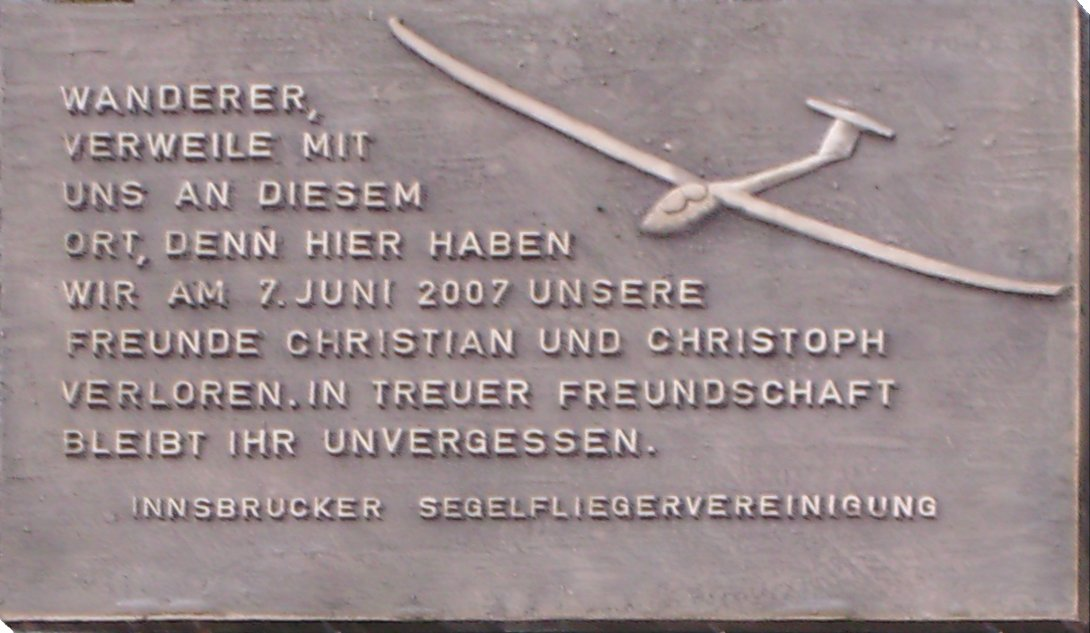
\includegraphics[width=12cm]{png/CC}
\end{center}
47.0789$^\circ$N 11.3060$^\circ$E

\newpage
\tableofcontents
\sloppy

\section{Introduction}
\emph{GPLIGC} is a software package for glider pilots, hang- and paraglider pilots, and for all others,
who want to analyse and visualise GPS track logs.
\emph{GPLIGC} reads track logs from files in igc-format as specified by the International Gliding Commission \cite{igc}.
Extracting the data from the GPS devices and conversion to the igc format has to be done with third-party software.
(GPS tracks can be downloaded from some Garmin devices using \emph{gpspoint}~\cite{gpspoint},
Nokia/Symbian mobile phones can be used as loggers utilising \emph{gsil}~\cite{gsil}
and another option is to use \emph{gpsbabel} \cite{gpsbabel}).

The package contains two main programs: (1) \emph{gpligc}, analysation and (2) \emph{ogie},
3D visualisation (can also be used as a digital elevation data viewer).

The software can be used under the terms of the GNU General Public License (see appendix \ref{gpl}),
which means that it's free and the source code is available.
For details read the license, which is included in appendix~\ref{gpl}.

The webpage of \emph{gpligc} can be found at \cite{gpligc}.

\subsection{GPLIGC}
\emph{GPLIGC} is a flight data analysing software. Its name is assembled from \textbf{GPL} (the GNU General Public License, \cite{fsf}), \textbf{G}nuplot (free plotting software, \cite{gnuplot}), \textbf{P}erl (the famous scripting and programming language, \cite{perl}), \textbf{L}ogger (flight data recorder) and \textbf{IGC} (the International Gliding Commission and name of the flight data file format, \cite{igc}).
\emph{GPLIGC} is written in Perl \cite{perl}, using the Perl/Tk module \cite{perltk} for the graphical user interface.
Track and altitude plots can be visualised in a simple way and some basic statistical information can be calculated.
The recorded data can be analysed in detail.
Optimisation for the onlinecontest can be performed. Turn-point observation zones can be displayed.
\emph{Gnuplot} \cite{gnuplot} is used to generate some plots (barogram, GPS-altitude, vertical speed, speed, noise level, etc.) of the data either to the screen or some graphical file format (including png, fig, ps, eps).
\emph{GPLIGC} is able to locate coordinates of photos, which have been taken with a digital camera, while logging GPS data.
To use this geo-tagging feature a correct timestamp in the JPEGs EXIF header is needed or it should be retained as the files timestamp.

The development of \emph{gpligc} started in January 2000.


\subsection{OGIE}
\emph{OGIE} is a  program written in C++ using OpenGL and GLUT (or freeglut \cite{freeglut}) libraries.
The flight data can be visualised in 3D (even in \emph{real 3D}, using stereoscopic methods).
The viewpoint can be controlled in several  ways (egocentric, swivel/rotate or coupled with the flight).
Digital elevation models can be used to display the terrain, digitised maps can be used, and airspaces from OpenAir\texttrademark-files can also be displayed.
Colour scaling can be applied to the terrain data, the digitised maps and to the flight-track itself.
\emph{OGIE} can also be used as a digital elevation model viewer.
\emph{OGIE} is able to render offscreen. Images can be generated hardware accelerated, or hardware independent (with Mesa \cite{mesa}). This can be used to generate images for contests etc. (server use).
\emph{OGIE}s name was assembled from \emph{\textbf{o}pen\textbf{G}L\textbf{I}GC\textbf{e}xplorer}: \textbf{openGL} (the open Graphics Library), \textbf{IGC} \cite{igc}, \textbf{explorer}.


The development of \emph{ogie} started in 2002. Until 2010 the long name \emph{openGLIGCexplorer} was used.


\paragraph{How they work together}
Basically \emph{gpligc} and \emph{ogie} are independent pieces of software.
\emph{OGIE} was designed to be an independent 3D visualisation-only tool, because Perl is too slow for that task.
However, if you start \emph{ogie} from within \emph{gpligc} some data (altitude calibration data, marked lifts, etc.) will be put forward to \emph{ogie}.
%But if you start the \emph{openGLIGCexplorer} by the button in \emph{GPLIGC}, there will be some communication between them...

\subsection{Contact, bug reports, feature requests}
Bug reports and feature requests should be submitted via the \emph{gpligc} support page at Sourceforge \cite{gpligc}.
I recommend to sign up for the \emph{gpligc-announce} mailing list \cite{gpligc}, which I use to inform users of updates or serious bugs, etc. (very low traffic)

\section{Requirements}
\label{requirements}

\subsection*{GPLIGC}

\begin{itemize}
\item Perl~5 with the Perl~Tk module \cite{perl,perltk}
\item {\scriptsize optional:} Gnuplot \cite{gnuplot} (used to produce 2d and 3d diagrams and plots of the data)
\item {\scriptsize optional:} Perl modules \texttt{Imager} \cite{imager} and \texttt{Image::ExifTool} \cite{exiftool} for full functionality
\end{itemize}


\subsection*{OGIE}

\begin{itemize}
\item OpenGL graphics (e.g. Mesa3d \cite{mesa})
\end{itemize}


\subsection*{Platforms, software versions}
GPLIGC is developed/built and tested on following platforms with given software versions.

\begin{itemize}
\item Linux: x86\_64
\item OpenBSD: 5.5 (amd64)
\item Windows: Vista (XP, Windows~7, and Windows 8/10 [not yet tested])
%\item Mac OS X: 10.4/10.5 \red{not tested for a long time}
\item gcc: 4.9 %linux gentoo
\item Perl: 5.20, %linux
(Windows: Strawberry Perl 5.22, 32bit)
\item Perl Tk: 804.033
\item Perl modules: Imager: 1.004, %
Image::ExifTool: 10.10
\item Gnuplot: 4.6 (Windows: Gnuplot-4.2.6 is included)
\item Mesa3d: 11.0.6 (Windows: native openGL is used)
\item freeglut: 3.0.0 (Windows: dll is provided)
\item {\scriptsize optional} gpsd: 3.15 (GPSD\_API\_VERSION 5)
\item libjpeg (e.g. libjpeg-turbo 1.4.2, jpeg 9a)
\item built platform windows: MinGW32 (1.0.18)
\end{itemize}

\section{Installation}

\subsection{General Linux and Unix installation procedure}
\label{unix_install}
\label{linux_install}

This applies to all Linux and Unix operating systems.

\begin{enumerate}

\item Extract the archive: \\
\texttt{tar xvzf gpligc-version.tar.gz} \\
%\texttt{tar xvzf GPLIGC-version-os-arch.tar.gz}, in the case you're using a package containing binaries.\\
Change to the just created directory: \\
\texttt{cd gpligc-version}

\item Configure and build the software:\\
\texttt{./configure}\\
for options and details on configuring the build see README and the output of \texttt{./configure --help}

\item Build the software:\\
\texttt{make}

\item  \label{root}
Become root or run the next command using sudo.\\
\texttt{make install} %\quad or execute the script in the next step using \texttt{sudo}.
%%%%%%%%%%%%%%%%%%%%%%%%%%%%%%%%%%%%%%%%%%%19 proofreading till here

%\item  start the installation script: (If you have security concerns, feel free to review the script before)\\
%\texttt{./install.sh} \\
%Some of the gpligc packages include binaries for the named platform.
%The install script will check them.
%If they don't work some parts of the software need to be compiled.
%However, you can chose to compile anyway, ignoring the shipped binaries.
%The src-package dont contain any binaries and need compilation in any case.

%If no binaries are found (or if the binaries don't work for some reason)
%The script will compile the  binaries (if this fails you will find more details in section ~\ref{compile}). \\
%The script will ask you for \\
%a) an installation prefix (/usr/local is recommended) \\
%If the script is allowed to write, it will install gpligc and ogie,
%files of installed earlier versions will be overwritten (if the same path is used).

\item copy the example configuration file
\texttt{.ogierc} (PREFIX/share/gpligc/) to your HOME directory
and edit it according to your needs (see section~\ref{config}).

\item \textbf{attention} re-using old \texttt{.gpligcrc} may cause problems, see section~\ref{bugs}. To be sure just delete your old configuration
file: \texttt{rm \textasciitilde/.gpligcrc}.

\item Make sure that Gnuplot \cite{gnuplot} is installed and in the path.
GPLIGC will also work without Gnuplot,  but you will not be able to use the plotting features.

\item Make sure that the Perl/Tk \cite{perltk} module is installed

\item Read the documentation to learn how to use gpligc \& ogie

\end{enumerate}


%\subsubsection{Compiling ogie}
%\label{compile}
%OGIE should be compiled from within the install script. If that fails, you'll find some more information here.
%Furthermore, you'll find some information here, how you can compile a `mesa-only offscreen binary', which can be used on a headless server.

%The C/C++ parts (everything that needs compilation) of the ogie is located in the \texttt{openGLIGCexplorer} subfolder.

%\texttt{make help} will give you an overview of the available targets in the makefile.
%In general you should try to use one of the \emph{all-*} targets, closest matching your platform.
%If that fails, you need to modify the \texttt{Makefile} or contact the author.

%\paragraph{Compiling a statically linked binary (Mesa3D)}
%This is only needed if you're going to use ogie on a server for offscreen rendering (like the onlineplotter).

%Static linking with Mesa is possible and tested for linux and windows (cygwin) and requires at least \emph{Mesa 5.0.1}, (4.x seems not to work with ogie and offscreen rendering).
%\red{However, be warned it is a pain to get it linked.}

%\subparagraph{Mesa 7.0.3} works fine, as tested. If you need larger than 4096x4096 pictures (e.g. to create cool posters) you have to change
%the maximum sizes in \texttt{src/mesa/main/config.h} (in the mesa source code, before compiling mesa):
%\texttt{\#define~MAX\_WIDTH~32768} and \texttt{\#define~MAX\_HEIGHT~32768}.

%\subparagraph{Mesa 7.4.1} tested in May 2009. It worked for me as follows: download and unpack MesaLib and MesaGLUT-7.4.1. Change the maximum width and height as described above. Use \texttt{make linux-x86-64-static} or a similar target. After Mesa compiled, \texttt{cp lib64/lib*.a \textasciitilde/lib/} to put the static mesa-libs in your private \textasciitilde/lib/.

%For further details see the ogie Makefile. \texttt{MESAPATH, GLEX\_OSMESA} and \texttt{GLEX\_OSMESA\_WIN} are interesting bits.
%The osmesa target in the Makefile requires the static Mesa libraries in \textasciitilde/lib/

%\begin{verbatim}
%make clean
%make osmesa
%\end{verbatim}

%Compiling this on windows/cygwin is even more painful. However, I succeeded once, see comments in the Makefile.
%\begin{verbatim}
%make clean
%make osmesa-win
%\end{verbatim}

%The binary, which will be build is called \emph{openGLIGCexplorer-mesa}.



%\subsection{OpenBSD}
%On OpenBSD platforms, you need to install the following packages: gmake, p5-Tk, gnuplot, jpeg, bash.
%You'll need the glut library too, which is not available as a packge, but from the ports.
%The install.sh script should be started with the bash shell: \\
%\texttt{sudo bash ./install.sh}

%\subsection{Gentoo Linux}
%Gentoo users may use the gpligc ebuild from the \emph{sunrise} overlay.\\
%Adding the sunrise overlay: \texttt{layman -a sunrise} (for details see gentoo/layman documentation)\\
%Installing gpligc: \texttt{emerge gpligc}


%\subsection{Mac OS X}
\label{mac}
This paragraph is mainly written by Matthew Hoover. Also he was the one, who did the testing while gpligc/ogie was ported to Mac OS X.
Owing to his efforts, binaries for ppc- and intel-based Mac OSX machines can be provided.
Thanks a lot, Matthew!

Another section was added by Michael Schlotter, who describes how to install ogie/ogie without using fink.
For that reason Perl/Tk and Gnuplot have to been build from sources. Thanks Michael!


\subsubsection{General}
In order to get gpligc running, you need Perl with the Perl/Tk module. This usually requires to have X11 installed, since Perl/Tk doesn't work with the native Mac OSX GUI (Aqua).
As you also have to install gnuplot, I recommend the easy way shown in section~\ref{fink} using the fink platform.
If you're a more experienced developer (not using fink), you may want to compile Perl/Tk and gnuplot by yourself.
See section~\ref{schlotter}.
To compile the ogie binaries on your machine, you'll need some developer tools (as gcc, make, etc.).
So far, I didn't find a way not to use the jpeglib from fink (if you know, please report).


\subsubsection{Matthew's howto, using fink}
\label{fink}
\begin{enumerate}

\item  Install X11 from the Tools disk included with the OSX package. \\
(X11 is the unix X-Window system and is needed for the  Perl/Tk-stuff (for gpligc)).

\item  Install fink \cite{fink}. \\
Fink is a packaging system that allows Mac users to install, compile and use a wide range of free software.
We need this to install gnuplot and the Perl/Tk-module.

    \begin{enumerate}
        \item  If the user is unfamiliar with fink then also install fink
                commander which is a GUI front end for fink.
        \item  Make sure that the fink or fink commander is able to install
            "unstable" packages.
            You have to modify \texttt{/sw/etc/fink.conf} (Add main/unstable to the line containing "Trees:")
            More can be found in the fink documentation.
    \end{enumerate}

\item  Install and compile the Perl/Tk module. Therefore you have to check which Perl is installed on your system (\texttt{perl -V}).
    There are different Perl/Tk-module versions (and I am not sure if the newer ones will work with older perls...)
    According to your installed perl choose one of tk-pm560, tk-pm580 or tk-pm581. This example will continue with tk-pm581.\\

Install the tk-pm581 package using fink (\texttt{fink install tk-pm581}) or fink
commander.  There are also tk-pm581-bin and tk-pm581-man.  These will
be installed and compiled and archived when the first is selected.  If
gpligc will not run try unpacking these also.

\item  Install gnuplot using fink (\texttt{fink -b install gnuplot}) or fink commander.  I used the last
stable version with the binary files because it is faster although
there is a newer unstable version.

\item Now you can proceed with the instructions for Unix (see \ref{unix_install}) installation. Be aware to use a binary package for Mac OS X. 
The installation paths will be different from those used in Unix/Linux instructions.
For the installation prefix  you can choose by yourself (maybe /sw or /usr).

\item  To run, open X11 and then Terminal.  GPLIGC must be started from
within Terminal and X11 must also be running because it will not be
automagically started.

\item You should add \\
\texttt{test -r /sw/bin/init.sh \&\& . /sw/bin/init.sh} \\
to your \texttt{.bashrc} file to start gpligc in a xterm shell
without a terminal shell opened.

\end{enumerate}


\subsubsection{Michael Schlotter's howto}
\label{schlotter}

\begin{enumerate}
\item  Install Developer Tools from the Mac OSX Installation CD/DVD
\item  Download and install Apples X11-Server
\item  Install X11SDK and BSDSDK. This is done by double-clicking on
    \texttt{X11SDK.pkg} and \texttt{BSDSDK.pkg} in
    \textit{/Applications/Installers/Developer Tools/Packages}
\item Download, build and install gnuplot 4.0.0.
    Don't worry if \textit{make-check} produces some errors.
\item Download, build and install Perl/TK. I used \texttt{Tk-804.027.tar.gz}.
    Don't worry if \textit{make-test} produces some errors.
\item Download and install the latest gpligc with precompiled binaries for Mac
\end{enumerate}


\subsection{Windows XP/Vista/Win7/Win8}
\label{windows_install}


You'll need Perl. If unsure which Perl distribution to use, read section~\ref{perl}. But you need Perl before you proceed!

\begin{enumerate}

\item Unzip the GPLIGC-version-win32.zip archive to a temporary location
(maybe you have done that already).
Open this location in the Explorer and double-click the install-script: \\
\texttt{install\_windows.pl} \\
(if *.pl scripts are not associated with the perl-interpreter already,
you can try "open with", select browse and find bin/perl.exe in the
perl-install directory). \\
\textbf{Attention!} Don't run the install script from within the zip file. That method will not work!
Unpack the zip archive in any case and run the script from the unpacked directory.

\item The Installation script will ask you for a location to install.
Let the script do the following work for you:
a) copy all files to the install-location
b) set some environment variables by adding them to the registry.

% either by setting them in
%\texttt{autoexec.bat} (Win95/98/ME) or

\item If the installation script fails, and tells you to set the environment Variables
by yourself:\\
Make sure that an environment variable GPLIGCHOME is set,
which contains the full absolute path to the GPLIGC-directory:\\
For example: \\
\texttt{c:$\backslash$some$\backslash$path$\backslash$GPLIGC} \\
And add the gpligc-directory to your PATH \\
How to set an environment variable: \\
a) Windows NT, 2000, XP, Vista: \\
Start - Settings - Control Panel - System (Advanced) - Environment... \\

%b) Windows 95, 98, ME: \\
%You have to add a line to the "c:$\backslash$autoexec.bat": \\
%set GPLIGCHOME$=$C:$\backslash$some$\backslash$path$\backslash$GPLIGC

\item You can remove the temporary directory, where the zipfile was extracted.

% GNUPLOT 4.2.6. is included in the package from 1.10pre7.
% seems to be the last available version with static wgnuplot.exe
% from 4.4 wgnuplot needs a bunch of dlls.

%\item If you do not have Gnuplot installed already, do so.
%Get it from the gnuplot page \cite{gnuplot} (get the win32 zip, e.g. \texttt{gp425win32.zip}).
%Installation is simple: just put the file \texttt{bin/wgnuplot.exe} in a location which is in the path
%(or the gpligc install location) \\
%\textbf{ATTENTION!} The executable file of the older gnuplot \emph{3.7.x} is named \texttt{wgnupl32.exe}. If you use
%the older gnuplot, you have to change the setting for the configuration key \texttt{gnuplot\_win\_exec} to \texttt{wgnupl32.exe}
%in \texttt{gpligc.ini} (for details see \ref{gpligcrc}).
%However, you should consider updating to gnuplot 4.x, since there are new nice interactive features like zooming, rotating of 3d-plots etc.
%The later gnuplot version (4.6) are shipped with an installer, which is easy use.


\item Edit the configuration file \texttt{ogie.ini} if you like to use a digital
elevation model, digitised maps, waypoints and/or airspace files.

For details read sections \ref{dem}, \ref{maps}, \ref{wp} and \ref{airspace}.

\item Create a shortcut to \texttt{GPLIGC.pl} on your desktop if you like

\end{enumerate}


%\paragraph{Notes for Windows 95, Windows ME}
%Support for these platforms is discontinued.

%GPLIGC has not been tested with Windows 95 and ME. On Win95 you probably will need the OpenGL libraries from Microsoft, because the early win95 versions do not have OpenGL support. Windows ME should work (maybe someone
%can verify that and write an email to me?)
%\paragraph{Notes for Windows 95, 98 and ME}
%These platforms will not be supported in the future.
%The cygwin environment (which is used to build the package on windows systems) will soon be updated from version 1.5 to 1.7.
%With that update support for the older windows systems will be discontinued.
%If you want to use openGLIGCexplorer on old windows systems, you should maintain a working cygwin 1.5 installation to build openGLIGCexplorer.


\subsubsection{Perl on Windows}
\label{perl}
There are two (probably even more) important Perl distribution for windows systems:
(1) Strawberry Perl \cite{strawberryperl}, which is a open-source distribution, with an easy-to-use installer.
I personally use this and recommend its use for gpligc.
(2) ActiveState ActivePerl~\cite{activeperl}, which is a closed-source distribution (but free for personal use).
On ActiveState Perl you can use the ppm package manager to install the needed modules (Tk, Imager, Image::ExifTool).

\paragraph{Strawberry Perl}
After downloading the msi installer package of Strawberry Perl (see~\ref{requirements} for specific version),
the installation is straight forward.
Then, open a cmd.exe command-window (or perl commandline from the strawberry program folder) and enter the following
command to install perl Tk:\\
\texttt{ppm install Tk}\\
You can also use CPAN to install Tk, like the other modules below (however, this will take a couple of minutes more, as it will compile the Tk module from scratch).
To install the additional modules use the CPAN client (strawberry perl / tools) and enter the following commands
at the CPAN promt:\\
\texttt{install Image::ExifTool}\\
\texttt{install Imager}  $\leftarrow$ in recent strawberry perl this is included already.\\
Done!
Anti virus software may need to be disabled during CPAN installs (caused errors on my system).


%\paragraph{ActiveState ActivePerl}
%You can't use the new cool map-feature of gpligc if you decide to use this one! (If you're a more experienced Perl/Windows user, you may try to fix the lack of png support in the Imager module, or maybe ActiveState will ship a proper-built Imager module one day... --- let me know).
%Download and install the ActiveState ActivePerl from \cite{activeperl}.
%If your Active State Perl version is later or equal 5.10, you have to open the Perl Package Manager and install the Tk (804.029) module.
%Tk is not shown in the default list, you have chose `all packages' from the view menu.



%\subsection{Update installation}
%If you want to update from an earlier version, you can safely use the install-scripts. Executable files will be replaced.
%Your data and configuration files will not be overwritten.
%But be sure to use the same paths for installation and symbolic links as in the previous installation, otherwise you my have conflicting installations.


\subsection{Additional Perl modules}
For best experience with gpligc you should install the following Perl modules:\\

\begin{itemize}
 \item \texttt{Image::ExifTool} \quad needed for photo-locator and geo-tagging. See \cite{exiftool}.
 \item \texttt{Imager} \quad needed for the new (1.9) map-feature. See \cite{imager}.
\end{itemize}

there are (at least) two ways of installing Perl modules

\subsubsection{manually} You should go to the CPAN \cite{cpan} and search for the modules, download and install them.
 After downloading the archive(s), it takes the usual three commands: \\
\texttt{perl Makefile.PL} \\
\texttt{make} \\
\texttt{make install}   (as root)\\


\subsubsection{using the CPAN.pm module} If the cpan module isn't configured yet, this can be done interactively or even automated during this process. \\
\texttt{perl -MCPAN -e shell} \\
then enter \\
\texttt{install Image::ExifTool}\\
at the cpan prompt.


%moved to ogie-chapter
%       %$Id: dem.tex 3 2014-07-31 09:59:20Z kruegerh $
%;;; Local IspellDict: "british"


\subsection{Digital Elevation Model}
\label{dem}

There are many digital elevation models on the web, which can be downloaded for free and used with ogie:
ETOPO2 \cite{etopo2}, GLOBE \cite{globe}, GTOPO30 \cite{gtopo30}, SRTM30 Plus (TOPO30) \cite{srtm30plus}, SRTM30 \cite{srtmv2}, SRTM-3 \cite{srtmv2} and SRTM-1 \cite{srtmv2}.
GTOPO30, SRTM30 (Plus) and GLOBE have a resolution of 30 arc-seconds, 1km.
ETOPO2 has a 2-minute grid (4km), but also covers the oceans.
SRTM-3 is 3 arc-seconds (90m) and SRTM-1 (only available for U.S.) is 1 arc-second (30m).

The "Shuttle Radar Topography Mission" (SRTM) topographic data
with resolution 1 arc-second (for USA) and 3 arc-second for almost the rest of the world
is available, but due to the high resolution not very good for regular flight-analysis. (Graphics
hardware won't handle larger areas).

My recommendation is to use either GTOPO30 or SRTM30 (Plus). 
If you have lots of hard disk space and want to analyse flights from many countries, you should consider
to build a \texttt{WORLD.DEM} from GTOPO30/SRTM30. If you like to explore the oceans, you may merge
it with ETOPO2 data. Data of this type is available from the gpligc download directories for many countries (including needed configuration settings).

SRTM-3 and SRTM-1 can be used for small-scale high-resolution application.


\subsubsection*{Data format}

Binary data in 2 byte integer (big endian byte) format is needed.
(You can get these directly from GLOBE, GTOPO30 and ETOPO2 Web sites)
Little endian data can be used with the config option: \texttt{BIGENDIAN false}.


\subsubsection{GTOPO30, SRTM30}
The worldwide GTOPO30 \cite{gtopo30} elevation model is split up in 33 pieces (tiles).
Get the "tile" you need and put the full path to the *.DEM file into the
configuration-file (see \ref{demconf}). You also need to set the rows and columns
and minima and maxima and grid resolution.

If you have lots of space on your hard-disk and a fast internet connection you should consider to
get all (33) tiles (about 280~MB compressed) and use the \texttt{createworld}
tool to generate a \texttt{WORLD.DEM} (single file containing worldwide elevation data, really cool!) file:

\begin{enumerate}
\item "\texttt{tar xvzf}"  all tiles into one directory (taht will need more than 2 GB).
      You only need to extract the *.DEM files from the *.tar.gz archives
      downloaded from GTOPO. Use the following cmdline (in the directory with
      all archives) to extract *.DEM files only: \\
      \texttt{find . -name '*0.tar.gz' -exec tar xvzf \{\}  *.DEM ';'}

\item invoke \texttt{createworld} in the same directory (this will need another 1.8 GB)
      
\item enjoy the 1.8 GB (!) \texttt{WORLD.DEM} (check \texttt{WORLD.DEM} for its size:
      should be 1.866.240.000 bytes)

\item settings for the \texttt{WORLD.DEM} can be found in the default-config file

\end{enumerate}

Now there is an improved SRTM30 model, which is based on the shuttle radar topography
mission. Basically, the SRTM30 seems to be a better GTOPO30. The SRTM30 data is also available
for free  and can be used to build the \texttt{WORLD.DEM} as described above. SRTM30 data didn't cover
the regions south of 60$^\circ$S. To obtain a \texttt{WORLD.DEM} file you should take the 6 arctic
tiles from GTOPO30, the remaining 27 from SRTM30.


\subsubsection{ETOPO2 (and merging it into the GTOPO30)}
If you have created a \texttt{WORLD.DEM} (1.8GB) datafile as described above, you can merge it with the bathymetry(sea-depth)-data from etopo20 \cite{etopo2}.
Get the \texttt{etopo20.i2.gz} file from the web. "Gunzipped" it has 116.672.402 bytes.
Put the \texttt{WORLD.DEM} and the \texttt{etopo2.i2} in the same directory and call (within that directory) \texttt{etopo2merger}, which will merge them into a \texttt{WORLD3.DEM} file.
Because the ETOPO2 resolution is lower than the resolution from GTOPO30, the additional data-points are obtained by interpolation.

\subsubsection{GLOBE}
Download the region you need (freely selectable \cite{globe}) and make sure that you
get the right data format. In the *.hdr file (which you will get too,
you can find all needed information to edit the config-file.

These are the options to be selected at GLOBE download page:\\
FreeForm ND\\
int16\\
Mac/Unix Binary\\

the data file is called   *.bin
the *.hdr file contains some information you need to edit the
ogie configfile.


\subsubsection{SRTM30 Plus (TOPO30)}
The SRTM30 Plus \cite{srtm30plus} elevation model is a merged SRTM30 and GTOPO30, including bathymetry data from several sources.
It can be downloaded as a single (1.8GB) data file from \cite{srtm30plus}.
Notice the different settings for DEM\_LAT\_MAX and DEM\_LON\_MIN! (differing from what should be used for SRTM30 and GTOPO30 world files).
See example configuration file!

\subsubsection{SRTM-1 and SRTM-3}
SRTM-3 (3 arc-seconds) data is available for free (for north and south-America and for Eurasia). SRTM-1
(1 arc-second) is available for the USA. The data is in .hgt format which is exactly, what ogie
can read. But the data is tiled into 1x1 degree pieces. This might be useful for high resolution analysis of
some terrain detail, but is just too much data for normal (glider-)flight analysis.
However, you'll find it at \cite{srtmv2}.
The Documentation folder will give you important information about data-format etc.


\subsubsection{SRTM-1 and SRTM-3 finished from seamless server}

From the usgs seamless server \cite{seamless} you can get these data.
It can be downloaded in a binary .bil format, which is accompanied by a .blw file, which contains additional information. Attention, there is a half-pixel shift.
The actual coordinates for the upp-left corner can be found in the last two lines in the .blw file.
It seems that void areas are set to 0, in contrast to the original \emph{research grade SRTM data} which uses -32768.
Additionally you will need \texttt{BIGENDIAN false}.


\subsubsection{USGS DEM (30-m and 10-m)}
\emph{This section is written by} \textsc{Vit Hradecky,} \emph{thanks} \\

Digital elevation data with 30-m and 10-m resolution for the U.S. is
now available for free at \cite{geocomm}.
The data is broken up into the standard USGS 7.5-min quads. Most of the
data is in the newer SDTS format, while some of it is in the older ASCII
DEM format. Fortunately, a utility exists to dump either into a raw
binary file, which is readable by ogie. Compile the C source from
\cite{readdem} and execute \\
\texttt{read\_dem berlin10m.DEM.SDTS.TAR berlin10m.BIN berlin10m.HDR 0} \\
This will convert data for the Berlin USGS quad from the SDTS format to
the 16-bit binary format, output to berlin10m.BIN, dump the headers into
berlin10m.HDR, and set bad data to zero elevation. The output will be in
little-endian byte order. Use the \texttt{BIGENDIAN false} option in the
configuration file to read the data correctly. The DEM latitude and
longitude limits can be found in berlin10m.HDR.
The 10-m and 30-m data is in units feet rather than meters. Use \texttt{DEM\_INPUT\_FACTOR
0.30488} in the configuration file.


\subsubsection{Configuring ogie for DEM}
\label{demconf}

For details on the configuration file see \ref{config}.
This section will only describe the settings for the digital elevation model setup.

In the configuration file you need to specify the following lines: \\
The full path to the used digital elevation data file: \\
\texttt{DEM\_FILE  /full/path/to/demfile/W020N90.DEM} \\

The number of rows and columns of data \\
\texttt{DEM\_ROWS 6000} \\
\texttt{DEM\_COLUMNS 4800} \\

The maxima and minima of your DEM-File \\
\texttt{DEM\_LAT\_MIN 40} \\
\texttt{DEM\_LAT\_MAX 90}\\
\texttt{DEM\_LON\_MIN -20}\\
\texttt{DEM\_LON\_MAX 20}\\

And the resolution (0.00833333 for GTOPO30 and GLOBE)\\
\texttt{DEM\_GRID\_LAT 0.008333333333}\\
\texttt{DEM\_GRID\_LON 0.008333333333}\\
Divide by 10 for SRTM-3.

For other config-file options see \ref{config}.


%%% Local Variables:
%%% mode: latex
%%% TeX-master: "GPLIGC_manual.tex"
%%% End:

%       %$Id: maps.tex 3 2014-07-31 09:59:20Z kruegerh $
%;;; Local IspellDict: "british"

\subsubsection{Setting up digitised maps}
\label{maps}

Since version 1.2 the digitised maps can be in jpeg format.
The file extension should be .jpg (not .JPG or .jpeg etc).
The old rgb-format texture maps can be used too, but jpg maps should be preferred (they do not need that much diskspace).
Since version 1.3 the \texttt{NUMBER\_OF\_MAPS} is not needed anymore.


\paragraph{How to prepare maps}
First of all you have to use a scanner or digital camera to get your maps into the computer (or just download stuff from the web).
To avoid differences due to projections, the map should not be in one big tile, but many small pieces. The smaller the better. For a 1:500.000 map (like ICAO) pieces of 40' x 40' are a good choice (1$^\circ$ x 1$^\circ$ is probably also OK).
For the further processing of the digitised maps a good image manipulation software is needed such as Gimp (the GNU image manipulation program \cite{gimp}).
The pieces have to be cut out from the scanned raw image(s).
Then the pieces have to be straighten out, to avoid any distortions. The latitude or longitude should be constant for each border.
I use the transform tool (which can be used to straighten out perspective
distortions etc) to define a (distorted) box along the gridlines of the
40'x40' box, as exact as possible. The transform tool will straighten this
out to a perfect rectangular box: the map-tile, which should be scaled to
some power-of-2 width and height (128x256 or 256x512 or 512x512 or 512x1024
or or...) otherwise this has to be done internally in ogie, which will slow down things a little.
Furthermore, you need to know the coordinates of each border.
Then save the map tile as jpg image.

\paragraph{Set up the \texttt{.ogierc} file}

For each map-tile the full path to the image-file and the coordinates of the top, bottom, left and right border have
to be given in the configuration file.
You need to have a section (as follows) for \emph{each} map-tile:

\begin{verbatim}
   MAP_FILE /usr/local/gpligc/maps/bremen.jpg

   MAP_TOP 53.5
   MAP_RIGHT 9.3333333333
   MAP_LEFT 8.6666666667
   MAP_BOTTOM 52.8333333333
\end{verbatim}

The maps can be grouped in sets. You may want to have a map-set for each airfield you fly from.
Another way to use this feature would be to spilt large areas into multiple map sets, if you don't have enough video memory to display all maps at the same time.

Exampls: You have 20 sections for 20 map-tiles in your configuration file.
Now you can put a \texttt{MAP\_CUT} between the first 10 and the second 10
map-tile sections to split into two map-sets.
In ogie you can switch between multiple map-sets by using the "c" and "x" keys.
You may specify more than two map sets by using multiple \texttt{MAP\_CUT}.

Every map-set can be named with \texttt{MAP\_SET\_NAME name} to select it at startup with \texttt{--map-set-name name}, or by its name from the menu.


\paragraph{shifting individual map tiles}
$\,$ \\
\texttt{MAP\_SHIFT\_LAT  degrees} \\
\texttt{MAP\_SHIFT\_LON  degrees} \\
If your maps don't fit exactly, a shift in latitude and/or longitude may be defined.
If  \texttt{MAP\_SHIFT\_...} is given, all following map tiles will be shifted by the given amount, until the shift
is set to zero or to another value.


\paragraph{rgb-format maps}
This shouldn't be used anymore... except you want to use your old maps,
or you don't like lossy compression.
Every map-tile can be in a headerless .rgb (3 byte per pixel) data-format (I
use Image Magick's "convert" to create that format). The size has to
be $2^n$ x $2^n$. That means   you have to scale the image before. Width and height
should be a power of 2 (pixels).
Because the rgb-format is headerless it cannot contain the information about the size
of the image. You need to specify MAP\_WIDTH and MAP\_HEIGHT for each map-tile in your
configuration file.
There is a limit for the maximum pixels for each dimension (width and height).
You can query this limit by executing \texttt{ogie -q}.
Look for \texttt{GL\_MAX\_TEXTURE\_SIZE} [both values (width and height) have to be less or equal
to \texttt{GL\_MAX\_TEXTURE\_SIZE}].


%%% Local Variables:
%%% mode: latex
%%% TeX-master: "GPLIGC_manual.tex"
%%% End:

%       %$Id: airspace.tex 3 2014-07-31 09:59:20Z kruegerh $
%spellch 1.8
%;;; Local IspellDict: "british"


\subsection{Airspace}
\label{airspace}

If you want airspace information to be displayed, you should get an OpenAir\texttrademark\ airspace file (that's the same format as used by Winpilot) for your region and set up your \texttt{.ogierc} file.
One keyword declares  the filename of the airspace-file, another one sets the default, whether airspaces should be displayed or not. \\
\texttt{OPEN\_AIR\_FILE /path/to/OpenAir/file} \\
\texttt{AIRSPACE true} \\
An alternative way are the following command-line options \\
\texttt{--airspace-file=/path/to/OpenAir/file} and \texttt{--airspace} or \texttt{--no-airspace} to turn them on or off.

At runtime, airspaces can be switched on or off via the menu or by F9. Shift-F9 toggles the wire frame and transparent mode.

\subsubsection{How and where to get OpenAir files}
On the gpligc web-site you may find an airspace folder in the download area. Some OpenAir formatted files can be found there.
Another option is the page of J. Leibacher \cite{leibacher}.

% outdated
%\emph{I don't know whether the following paragraph is still valid!}\\
%Another option is to use the program of \texttt{Carl Ekdahl}, which can be found on the \emph{Soaring Server}.
%That program works on M\$-Windows only, but can create OpenAir formatted files from recent \emph{DAFIF} sources.
%To do that the dafift.zip is needed and the following files need to be copied to the right location inside the airspace-program %(from \texttt{Carl Ekdahl}) folders: \texttt{BDRY.TXT, BDRY\_PAR.TXT, SUAS.TXT, SUAS\_PAR.TXT}.




%%% Local Variables:
%%% mode: latex
%%% TeX-master: "GPLIGC_manual.tex"
%%% End:
%	\subsection{Waypoints}
\label{wp}

Waypoints can be displayed by ogie.
The file containing the waypoints can be declared in the ogie-configuration file by the keyword \texttt{WAYPOINTS\_FILE} or by a commandline argument \texttt{--waypoints-file}. Some more keywords and command-line arguments are available to change the default behaviour.

To switch them on or off use the F12 key. Page-up and page-down can be used to change the size of the spheres, the text-size can be changed with shift-page-up/down. Using shift-pos1 or shift-end changes the displayed text (waypoint-long name, waypoint short-name, waypoint-altitude, waypoint-symbol name).

\subsubsection{Format of the waypoint file}
As there are probably hundreds of waypoint file formats available, I chose a simple one, which I use with my handheld Garmin GPS and \emph{gpsbabel} \cite{gpsbabel}.
It has six columns of data: latitude (degrees), longitude (degrees), altitude (metres), short name (max six letters), long name, symbol name.
Columns are seperated by whitespaces (therefore no whitespaces are allowed within the names).
Using \emph{gpsbabel} it should be easy to convert any format to this.
You'll find a gpsbabel-style (\texttt{gpligcwpt.gpsbabelstyle}) file in the PREFIX/share/gpligc folder.
Here is an example how to convert a cambridge waypoint file to the needed format:\\

\texttt{gpsbabel -i cambridge -f cambridgefile  -o xcsv,style=gpligcwpt.gpsbabelstyle -F mywpts.gwpt}\\
The important part is the output format option `xcsv,style=' using the provided style file.\\
However, \emph{gpsbabel} is cool, you should have a look at it anyway.
You can even download your waypoints from a Garmin device like this:\\
\texttt{gpsbabel -i garmin -f /dev/ttyS1 -o xcvs,style=gpligcwpt.gpsbabelstyle -F outfile.gwpt}
  %label wp

%$Id: gpligc.tex 3 2014-07-31 09:59:20Z kruegerh $
%last spellchecked: 1.21->1.22
%;;; Local IspellDict: "british"


\section{GPLIGC}

\subsection{How to start gpligc}

\begin{itemize}
\item{Linux, Unix:}
GPLIGC can be started from the command line by typing \\
\texttt{gpligc}\\
or\\
\texttt{gpligc  igcfile.igc}

%\item{Windows}
%From the command line (\texttt{cmd.exe} command prompt): \texttt{perl GPLIGC.pl} (from within the gpligc-directory)
%or double-click \texttt{GPLIGC.pl} from windows explorer.
%If windows asks you what application to open it with, you'll have to find your perl interpreter
%(whereever/you/installed/perl/bin/perl.exe).

%You cannot avoid that a cmd window pops up too, just ignore or minimise it.
\end{itemize}

\subsection{Main Window}
The flight-track will be displayed here.
Crossmarks indicate a single data fix point.
The corresponding data is shown above.
The displayed data is based on the barometric altitude.
In the case, that the igc-file does not contain any barometric altitude,
gpligc will switch to GPS-altitude.
A message will inform you about this, and
the information ``GPS-Altitude modus'' is displayed.

\textbf{Attention!} Some of the key-shortcuts are case-sensitive!

To move the crossmarks/cursor/indicators use F3 (move forward), F4 (fast forward), F2 (backward)  and F1 (fast backward).

`\texttt{t}' toggles task-display.
`\texttt{r}' sets the Gnuplot-range (side-length can be chosen in the menu) to the cross-mark position,
`\texttt{c}' toggles waypoint-cylinders and sectors (on/off).

Before using the waypoint sectors and cylinders you should delete doubled waypoints which may occur in the task declaration. E.g. if departure and start location are equal, or finish and landing.
Otherwise the FAI sectors cannot be calculated properly (maybe I'll implement some auto-detection of that sometime).

`\texttt{z}' zooms in or out!
The 'distance to' can be changed by selecting a different waypoint in the task editor window.
You can define a task start and finish point with "s" and "f", these points are
used to calculate the task-speed. These points are marked with small black circles.
They are used to mark the begin and end of unpowered flight also.
gpligc will try to detect the begin and end of unpowered flight, but this may fail sometimes and should be checked by the user.

Waypoints can be set with \texttt{a}, \texttt{b} or \texttt{p} (\texttt{b} adds before actual wp, \texttt{a} after and \texttt{p}
replaces the actual wp - actual wp is that one which is shown in the task editor window, if opened).

You can interactively zoom by selecting an area using the right mouse button. Return to full view using `\texttt{z}' key.
Select points by clicking in the barograph or the track, crossmarks will move to the selected position.
`\texttt{q}' will close the flight view window.
\texttt{Esc} exits gpligc

A list of the most important key-shortcuts can be accessed from the info menu.

\subsubsection{Layout}
%\red{not yet sure about this, after 2.0?!}
The layout of the main window can be changed in the following ways:
%(1) the help screen at the lower part can be disabled, if you don't need it any loger (set \texttt{fvw\_show\_help} "0").
the ratio of the heights of the track area and the barogramm area can be changed.
The config-key \texttt{fvw\_baro\_fraction "$n$"}, with $2 \le n \le 10$ sets the height of the barogramm to $\frac{1}{n}$ of the height of the track area.


\subsubsection{Task}
The task (which is given in the recent task definition; defined by the task-editor, via optimisation, or from igc-file) is shown regardless whether the waypoints are reached or not.
The task speed is calculated from the total task distance and the unpowered flight time, which may be adjusted as described above.

The third section will show the flown task, only way-points which you have reached are taken into account. A way-point is reached, if one logged data point is closer to the way-point as the cylinder radius (or 3km if only FAI sectors are chosen). The time of reaching the way-point is taken from the first point inside the way-point radius.
For exact analysis of speed you should use the F5, F6, F6 measuring function.
For each leg of the task the distance, speed, altitude gain/loss and the glide ratio (calculated from distance wp1-wp2 and altitude gain/loss) is displayed.


\subsubsection{Maps}
The usage of maps needs internet (if new maptiles have to be downloaded).
Changing the zoom or positions, will trigger automatic download of map-tiles, the window will be busy for a few seconds.

The display of maps can be activated or deactivated by key `\texttt{M}'.
The status lines at the top of the window will show the zoom-level and the number of tiles used.
If you want to change the zoom-level you can use the keys "$+$" and "$-$".
Changing the zoom-status will sometimes change the map-zoomlevel. This is needed to prevent
the use of too many tiles, or too large scaling of tiles.
The behaviour of this can be changed with two config-keys:
\texttt{map\_max\_tiles}
and \texttt{map\_max\_scalesize}, although not recommended.

The default map zoom-level is set by \texttt{maps\_zoomlevel} (recommended: 8).

Downloaded map tiles are stored in \texttt{.gpligc/maps}. Pressing the hash-key `\texttt{\#}' re-downloads the displayed map tiles.


\subsubsection{Postscript output}
output of flightviewWindow to postscript is possible by pressing `\texttt{o}' (flight-track)
or `\texttt{i}' (barogram)

\subsubsection{Resizing the window}
After resizing the window you need to press `\texttt{y}' to redraw the content (so far I couldn't find a suitable callback function in Perl/Tk).


\subsubsection{Statistics (thermals/glide)}
Thermal statistic (F8) will open two windows. One with some statistics and a
second one with a list of thermals (double click on a list-entry will jump
to that thermal in flight-view-window)
Glide statistics (F9) will open two windows. One with some statistics and a
second one with a list of glide-distances (double-click will jump to that
glide-distance)

\subsubsection{Statistics (selected range) and wind analysis}
(F5, F6, F7) can be used to set a first (F5) and a second (F6) point and
display some statistics (F7) for the selected range. The selected points will be
marked with small green circles and the time-span will be marked in red in the barogram.

To obtain a better view of the selected range press F11. The rest of the track will be omitted, and the
barogram will be zoomed to the selected range (F11 again will restore the previous view).

Furthermore, a difference plot of airspeed$-$groundspeed is performed via gnuplot. Even if no airspeed is present
(then its assumed as 0), information about the wind can be derived. The difference is plotted vs. the heading,
so select a range where many different headings are present (e.g. circling). A sinus function is fitted to the plot.

The amplitude of the sine function will give the wind speed, the direction can be read from the position of the maxima (direction of smalles ground speed).



\subsubsection{Save lifts / points of interest}
You may save interesting points (extraordinary lifts, wave-entry positions and the like) by pressing F10.
The actual position including altitude, vertical speed, time etc. is saved to \texttt{filename.lif}.
This file is being appended, so you have to delete it, in order to start from scratch.

This file can be used in ogie, and will be automatically loaded if ogie is started from within gpligc.


\subsubsection{Altitude calibration}
The barometrically recorded altitude is often shifted in respect to the real altitude.
In the simplest case, this is a constant shift (constant option).
To correct this, you can select a data point with known altitude
(e.g. before take-off, known airport elevation) and press `\texttt{e}'.
Then, enter the known altitude at this point, and the data will be shifted.
The barometric option will use a barometric model, the shift will decrease with altitude.
Chose the model according to your suspected error. Use `constant', if you have a constant systematic error in your altimeter.
Use `barometric' if the reference pressure is wrong.

The calibration data is saved withing the additional info (see section~\ref{add_info}).


\subsubsection{QNH and reference pressure calibration}
If your recorded track has the altitude referenced to MSL, you can enter an QNH (normalised pressure) to benefit from more accurate pressures and Flight Levels.
(Using key `\texttt{n}', entering only pressure for QNH, leaving 0 for reference pressure).

If you recorded track is referenced to a known pressure-level (e.g. 1013.25~hPa) you can change the reference to MSL by entering the reference-pressure and the QNH via `\texttt{n}'.


\subsubsection{View Photos / Multimedia}
By pressing `\texttt{v}', the closest photo or multimedia file will be displayed, either in
the internal viewer, or in an external one.

To set the viewer the configuration key \texttt{picture\_viewer} can be changed. ``internal''would tell
gpligc to use the internal one (only for pictures), every other value will be used as executable. For example you may use
``kuickshow'' or ``/path/to/any/strange/picture/Viewer/you/like/view''.
For other multimedia (audio recordings, movies) the configuration key ``mm\_player'' is used (defaults to mplayer).

To show/hide the files at the track, use key `\texttt{h}' in the flight-view-window to toggle. Pressing `\texttt{m}' will bring up a list of associated files.

\subsubsection{Photo time calibration and geotagging}
\label{photo_time}
Often, the clock of the digital camera (or cell phone) isn't exactly in sync with the `official GPS time'.
Therefore, we need to synchronise with the GPS time.
This can be done, if we have the exact time or position of one photo.
(I use to take one photograph of my GPS showing the GPS-time [preferrably UTC]).
The procedure in gpligc: (1) view the photo in question (using key \texttt{v}).
GPLIGC will remember it. (2) press `\texttt{x}' and enter the exact time (in UTC).
The determined shift will then applied to all photographs.
GPLIGC will write a file (\texttt{.GPLIGC-timeshift}) in the directory of the photos, so that this correction will be remembered.
To avoid all this the best method would be to have the cameras time in sync with the GPS-time. To make the correction easier it is a good idea to take a photo of your GPS showing the time.

After you have done the calibration you may want to geo-tag your photographs. Pressing \texttt{u} will do the job: The GPS coordinates will be written into the Exif headers of the images.
If any GPS tag is found (GPSAltitude, GPSLatitude, GPSLongitude or GPSTimeStamp) the file will not be altered.
If you want to overwrite existing GPS tags you have to set the configuration key \texttt{geotag\_force\_overwrite} to ``1''.


\textbf{Important!}  IGC files use UTC. Your camera probably uses local time. Therefore, gpligc has to know about your local time. The offset should be set in \texttt{.gpligcrc} (key "timezone"). The timezone offset can be set independently for each IGC-file using the \emph{additional flight info dialog} (see section~\ref{add_info}).
Once a calibration has been done, the calibration shift and time-zone offset will be saved in \texttt{.GPLIGC-timeshift} for that specific folder of pictures. In order to override the timezone from \texttt{.gpligcrc} one can create an \texttt{.GPLIGC-timeshift} in the directory with the pictures, containing two lines: line 1 should only contain 0 (thats the timeshift without timezone), line 2 should contain the timezone.
If your time-zone offset is so large, that the photos cannot be located on your tracklog, you should create \texttt{.GPLIGC-timeshift} file manually, containing a suitable time-zone offset and reload the picture-folder.


\subsubsection{Photo locator}
If the Image::ExifTool module is installed and the configuration key "photos" is active (=1, this is the default),
gpligc can locate pictures and show them next to the track, which allows you to identify the places where these pictures have been taken. Pictures not featuring an Exif header, may be located by the files timestamp, if thats retained.
When opening a igc file, gpligc will look for JPEG photos in the same directory, if there are none, gpligc will look in the
"photo\_path" directory (as set in .gpligcrc). The third and best method to tell gpligc where the pictures are, is to use the
"open photo directory" from the file menu. Just select one of the JPEGS there.
Since there is no date in igc files, you should point gpligc to photos from the same day. For more details about time-zone, and time offsets see \ref{photo_time}.


\subsection{Menus}

%% MENU
\subsubsection{File}
\paragraph{Open}
Select the IGC file to open.

\paragraph{Reload}
Reloads the opened IGC-file.

\paragraph{Download track (gpsbabel)}
Uses \emph{gpsbabel} \cite{gpsbabel} to download trackdata from a GPS-device.
The used command string can be defined using the configuration keyword \texttt{gpsbabel\_tdownload}.
For details see section~\ref{gpligcrc}.
%\red{Windows: I'm not sure whether this will work. Any users with gpsbabel out there for testing?}

\paragraph{Download garmin (linux only)}
Download GPS tracks from a garmin device, using gpspoint \cite{gpspoint}.
The gpspoint command has to be defined by the \texttt{garmin\_download} configure option (see section~\ref{gpligcrc}).
The track is then automatically converted to the IGC format by \texttt{gpsp2igcfile.pl} (see section~\ref{gpsp2igc}).

\paragraph{Download media (linux only)}
Use this option to download media files (audio recordings, videos, photos) from your mobile phone to locate them using GPS track.
You should specify your mountpoint and folders via \texttt{mm\_mountpoint} and \texttt{mm\_download\_dirs} (see section~\ref{gpligcrc}).

\paragraph{Export kml}
Exports the currently opened track to the kml format.

\paragraph{Export gpx}
Exports the currently opened track to the gpx format (useful for openstreetmap \cite{osm}).

\paragraph{Open photo/multimedia directory}
If your photos/multimedia files are not in the same folder as your GPS track, you can chose the folder here.



%% MENU
\subsubsection{Options}

\paragraph{Map settings}
For using maps, you need to have the Imager perl-module installed.
\emph{Use maps}, if enabled maps will be displayed in the flight-view-window.
This requires an internet connection, since maps are downloaded from the web.\\
\emph{Openstreetmap}, if set, openstreetmap will be used as map-server.
Openstreetmap data is \copyright\ OpenStreetMap (and) contributors, CC-BY-SA \cite{osm}.\\

The maps are downloaded to a subfolder in the directory, which is set by the config-key \texttt{map\_path}.
Don't change the names and folders there, since downloaded maps will be reused if gpligc can find them.

Other map sources and map layers may become available later.




\paragraph{Gnuplot settings}
%This menu is available only on Unix-machines. With windows Gnuplot 4.x will be used by default, for Gnuplot 3.x you have to follow the instructions given in section \ref{windows_install}. The Gnuplot-shell is not available on windows, sorry.
To use the new interactive features of Gnuplot 4.x you have to select the \emph{Gnuplot 4.x} option here. Highlights of these features are interactive zoom (right mouse-button) and interactive rotation of 3d plots.
The option \emph{Open Gnuplot-shell} will open a Gnuplot-shell for each plot, where you can do some more work on the plot. The  terminal application to be used can be changed by the configuration-key \texttt{gnuplot\_terminal\_app} the default is \emph{xterm -e} (see \ref{gpligcrc}).

Grid on/off controls the use of grid lines in Gnuplot.

\subparagraph{Draw Options}
Chose between \emph{Lines}, \emph{Dots} and \emph{Linespoints}. These are Gnuplot styles.


\subparagraph{Set terminal}
Select the gnuplot-terminal (corresponds to \texttt{set term ...} in gnuplot).
Some of the options may not be available in your gnuplot installation.
The x11 option (default) will put the plot on your screen.
All the others will write to a file. You will be asked for a filename (for
every plot). Specify the file name and extension in the save file dialog.

For more options on gnuplot exports use the Gnuplot-shell.


\paragraph{Optimiser method}
Different methods for the task optimisation can be chosen here. For details see section~\ref{optimise}.

\paragraph{WP cylinder}
Here you can select the type of waypoint observation zones; cylinders or FAI
sectors or both. For cylinders the radius can be chosen. Another option is to
turn the way-point names in \emph{flight view window} on or off.


\paragraph{WP-Plot side-length}
Selects the plot range for waypoint-plots (in gnuplot: the ranges used in x and y).
This also affects the size of the view in flight-view-window (if zoomed).
Options are 1,3,5 oder 10km. (In the flight-view-window the side length
is used in y-direction (latitude), the x-direction is scaled automatically to
prevent distortion).
If you use "Set range" (key r) in the \emph{flight view window}, this value will be used to set the
Gnuplot plotting ranges.

\paragraph{Set Noise Level Limit}
All recorded position fixes with a noise level above that limit will be
plotted in green (in flight-view-window).

\paragraph{Coordinate Format}
Here you can select the display format for the coordinates.

\paragraph{Speed, vertical speed, altitude and distance units}
Select your preferred units (km/h, m/s, m, ft, knots, ft/min)

\paragraph{Show accuracy}
If accuracy data is included in the IGC-file, you can active or deactive its use.
If activated you'll find additional output in the flight-view-window.

\paragraph{Photo locator}
Enables the photo locator feature. This feature can be used to geo-tag photographs, which were taken while the GPS-track was recorded.

\paragraph{Debugging output}
This option will dump tons of mostly useless text to your terminal. Use this if you like mystic numbers running down
your console. You should use this only when requested by the developers to track some bugs...

\paragraph{Save configuration}
The actual configuration settings (chosen in the options menu) will be saved to \texttt{.gpligcrc}.
Use this to make your setting permanent.

\paragraph{Reread configuration}
This will reread the \texttt{.gpligcrc} configuration file.
This option allows you to change some configuration setting with an text editor while gpligc is running.


\subsubsection{Plots-2D, Plots-3D}
This options will produce plots using Gnuplot.
Diagrams of the flight data will be written to 'term' (selected under "Set term").
Directly to X11 or after "Save-File-Dialog" to a file.

For changing the appearance of the output change the gnuplot-related options, or chose to open
a gnuplot-shell for each plot for further processing.
Gnuplot 4 also has some interactive features.

\subsubsection{Tools}

\paragraph{Flight info (IGC)}
Informations about the flight data recorder, pilot, plane and task will be displayed (as stored in the igc-file).
These comes from the IGC-file header.
The declared task from the IGC-file will be displayed too, but doubled way-points in task definition will be removed
(e.g. if take-off and start or finish and landing are the same)

\paragraph{Flight info (additional)}
\label{add_info}
Additional information (which is \emph{not} stored within the igc-file) can be viewed/edited here.
The data entered here can be stored in a \texttt{filename.gpi} file, which is automatically loaded, if found.
Useful to archive additional information on the flight.


\paragraph{Flight statistics}
Time of launch, landing, and flight will be available.
The time of the begin and end of unpowered flight is shown also.
The unpowered flight can be defined in flight-view-window with the keys \texttt{s} and \texttt{f}, or will be determined automatically (this may fail in some cases).

This section also shows calculations on the amount of oxygen, which should have been used according to \texttt{FAR 91.211}.
FAA requires 1l/min per 10.000ft (using a regular cannula or mask). Up to FL180 Oxymizer cannulas may be used (they use 1/3 of the oxygen, values given in brackets).
Four altitude bands are distinguished: \\
FL100--FL125 recommended use of oxygen\\
FL125--FL140 FAA requires oxygen in access of 30 minutes. Recommended: always \\
FL140--FL180 up to FL180 a cannula may be used.
FL180--FL250 only with mask (at higher altitudes you should have a demand-diluter system)\\
%\end{itemize}

The sum is given for recommended oxygen use (strictly from FL100) and FAA conform from FL125 (in access of 30 minutes) or FL140.

Don't forget to do the elevation calibration before calculating the statistics and to set the QNH (if you wan't it very precise).
For details of the calculation see the source code in \texttt{GPLIGCfunctions::OxygenStatistics}.


\paragraph{Task editor}
Select a waypoint of the current task and make 2d or 3d plots of it.
You can also delete waypoints from the task, or set the last wp equal to the first
one (to close a triangular flight etc.)


\subparagraph{Optimisations} \label{optimise} For all optimisations it is necessary to check that the begin and the end of the free (unpowered) flight is set correctly.
Otherwise waypoints my be set at a part of your flight, where you have been towed or using a motor.
To avoid that you need to set (or at least check the automatic detection) the "begin of unpowered flight time" to the beginning of the free flight (release point or engine-off point). The "end of unpowered flight time" needs to be set if you used an engine before landing.

The optimisation will only take the data between "begin of unpowered flight" and "end of unpowered flight" into account.
GPLIGCs optimisation routines are based on \emph{Metropolis Monte Carlo} (MMC) and/or \emph{simulated annealing} (SA) methods.
One of them can be chosen in the menu (the default can be set using the config key \texttt{optimizer\_method} to either "mmc" or "sa").

Several configuration keys can influence the algorithms.
\texttt{optimizer\_cycles\_mmc} and \texttt{optimizer\_cycles\_sa} define the number of optimizer runs for MMC and SA, respectively (each run is represented by one step of the progress bar).

\texttt{optimizer\_mmc} sets the commandline parameters for the optimizer run, if MMC is used.
\texttt{optimizer\_sa} sets the commandline parameters for the optimizer run, if SA is used.

If you want to play with that, check the source code of \texttt{optimizer.cpp}
In general, the default settings for both methods should find a close to optimal task.
I'm looking for feedback on their speed and reliability.
E.g. if they sometimes stuck at local maxima, missing the global one.

\texttt{optimizer\_verbose} and \texttt{optimizer\_debug} may enable the corresponding output of the optimizer at the console.

For brute-force calculation computers are still too slow, since a typical flight with about 5000 data records and a task of 7 waypoints, gives about $10^{22}$ solutions to check. The \texttt{optimizer} c++ code (see optimizer.cpp in the source) implements several experimental methods to find the best task.



\subparagraph{Optimisation OLC-classic (rules oct/2007)}
This will find the best task for OLC-classic (maximum points) and set it  as  the task.
The OLC-classic optimisation will find the probably best task with 7 waypoints (6 legs). The value to be optimised is the raw scoring: 4 legs with 1 point per kilometre, leg number 5 with 0.8 points per kilometre and the last leg with 0.6 points per kilometre. The altitude limit of 1000~m between the lowest point between "begin of unpowered flight" and the starting point and the highest point between the end point and the "end of unpowered flight" will be accounted  for.

\subparagraph{Optimisation DMST 2005}
This optimisation will find the best task according to the german DMSt 2005 rules. FAI tasks will be found, if possible.

This will not check for pre-flight declared tasks. It's still up to you, to check that. But if you've finished a pre-flight declared task, you probably will know.


\subparagraph{HOLC 2005}
This optimisation will find the best task (maximum points)  for the hang-gliding/para-gliding online contest (rules of 2005). Triangular
tasks, or FAI tasks will b used, if they'll have more points. Every logged data point is used (if it is valid).


% ????????????????????????????
\subparagraph{output of optimisation} If the optimisation is finished, a window with some information will appear.
Some of them need to be explained. Time of departure: This is the time of the lowest position after begin of un-powered flight and the first way-point (start-point). Finish-time: This is the time of the highest position after the last way-point and the end of unpowered flight.


\paragraph{OGIE -- 3d}
Starts ogie with the currently opened flight-data file
For details on ogie read section~\ref{ogie}

%%%%%%%%%%%%%%%%%%%%%%%%%%%%%%%%%%%%%%%%%%%%%%%%%
% ZZZZZZZ REMOVE THIS CRAP SOMETIME
%\paragraph{Logger read window (windows only)}
%\red{I don't know whether this still works, as I remember some problems with these small DOS programs on XP. Consequently, this feature will be removed in the future.}\\
%For each IGC approved logger a so called `small DOS program' has to be available for free.
%The small Windows/DOS (they don't even run on every Windows ...) programs can be downloaded at the FAI web-pages.

%To use these software from gpligc logger read window you should put the
%\texttt{data-xxx.exe, vali-xxx.exe} and \texttt{conv-xxx.exe} somewhere in your
%path (or in the gpligc installation directory, which should be in path).

%Use this with caution! I know that (for example) some versions of data-sdi won't work on XP.
%There may be problems with the others too.
%%%%%%%%%%%%%%%%%%%%%%%%%%%%%%%%%%%%%%%%%%%%%%%%%%%%%%


%\paragraph{OLC Flight claim}
%Online flight claims are no longer supported.
%This button will bring up a dialog box, where some information can be entered, which are necessary
%for the online contest. You have to choose the country for your olc flight claim. If you have used the optimisation before, you can
%use the task optimised by GPLIGC, otherwise the olc server will have to do the optimisation. After clicking OK, a web-browser will be started
%and you will be directed to the olc flight claim form with many values filled in already.
%The most important thing is, that the start and end of the un powered flight is set correctly. GPLIGC will try to check these automatically
%but sometimes the determination of the release time will fail! In the case you have used an engine after the flight and before landing
%(for example to avoid an out-landing) GPLIGC will fail finding the real end of un powered flight. Use the flight-view-window to check the
%begin and the end of the un powered flight and mark these points by \texttt{s} and \texttt{f}.

%\emph{This is tested for the normal online contest (gliders) only! I'm not sure about the claiming process for holc and dmst...}


%% MENU
\subsubsection{About/Info}
Copyright information and a link to the gpligc/ogie web-site












\subsection{The gpligc configuration file (.gpligcrc)}
This paragraph describes the new configuration file format of gpligc, which was introduced with gpligc 1.5.
Internally, gpligc stores all changeable configuration parameters in a `perl-hash'.
This is a data-structure, which is represented by pairs of keys and values.
Each key can be assigned to a value.
To get a valid \texttt{.gpligcrc} file, you should start gpligc and use options/save configuration.
This will write a \texttt{.gpligcrc} file, which includes \emph{all} valid keys and their default values.
The file has one line for each key-value pair.
The key is the first word, the value is enclosed in \texttt{"}.
The value can be changed with a text editor.
If you do this while gpligc is running, you need to select \emph{options/reread configuration} to trigger rereading of the changed configuration file.

%On Windows systems this configuration file is named \texttt{gpligc.ini}

Please refer to the section \ref{gpligcrc} to see what values are allowed.
If illegal values are used, gpligc may behave unpredictable or just crash.


%\subsection{Inter-process-communication with openGLIGCexplorer}
%This is disabled in 1.4, because of serious rewriting... Will be back in...
%Sorry not yet in 1.5.


\subsection{Remarks for using IGC files with gpligc}
GPLIGC does not check the integrity of the data.
Some calculations may not work as supposed, if there is more then one flight recorded in a in single IGC file
(e.g. the times of take-off, landing and flight duration will be wrong (starttime=starttime of first flight, landingtime=time of last landing)


%%% Local Variables:
%%% mode: latex
%%% TeX-master: "GPLIGC_manual.tex"
%%% End:

%$Id: explorer.tex 3 2014-07-31 09:59:20Z kruegerh $
%;;; Local IspellDict: "british"


\section{OGIE}
\label{ogie}

\subsection{Get started}
To start \emph{OGIE} press the "OGIE -- 3d" button in \emph{GPLIGC},
or type \texttt{ogie igcfile.igc} 
at the command line.% (xterm, console):\\% or MS-DOS prompt): \\

There are three different modes to use \emph{OGIE}:

\begin{itemize}

\item IGC-file mode:
You can give an igc-file as a single argument.
If you use more than one argument on the commandline, you need to specify
the igc-file by adding  \texttt{--igc-file FILENAME} (or \texttt{-i FILENAME}).

\item Terrain viewer: Select the centre of your view with  \texttt{--lat} and \texttt{--lon}. The size of the area can be selected with the following options: \texttt{--border, --border-lat, --border-lon}

\item GPS live view: Use the option \texttt{--gpsd}. \emph{ogie} will connect to the local gpsd \cite{gpsd} and obtain positional information for a live display of your location.

\end{itemize}

\subsection{Menus}
The pop-up menu is accessible by pressing the right mouse button in the \emph{OGIE} window. Most important options can be changed here.


\subsection{Mouse control}
The direction of view can be controlled with the mouse, the mouse pointer is invisible and cannot leave the window, unless
mouse control is disabled by pressing m.

Moving the mouse while the left button is pressed will result in rotating your position around the centre of the scene or around
the position of the marker (if activated). Dragging the mouse up and down, with the middle button pressed, will shift your
position towards or away from the centre or the marker position (if marker is activated).


Moving while the middle and left mouse button is pressed will shift the scene.


\subsection{Joystick control}
%A joystick is supported on Windows platforms via GLUT. 
On Unix/Linux (X11) the joystick can not accessed via GLUT (because
GLUT never supported joysticks on X11). If you want to use your joystick on X11, you have to install freeglut \cite{freeglut}.

The joysticks x,y and z-axis will move the viewpoint to the side, forward-backward and up-down. How much the viewpoint
will be shifted can be set in the configfile (JOYSTICK\_FACTOR\_X,Y,Z, see \ref{config}).

\subsection{Keyboard control}
For information on the Keyboard functions you should read the section \ref{keys}.
In the pop-up menu a \emph{help} is present, which will show the most important keys.
If you like to change the controls, edit in \texttt{KeyPressed} and \texttt{specialKeyPressed}-functions in
\texttt{GLexplorer.cpp} and recompile.

If you need the mouse pointer, it can be made visible by pressing key \emph{m}.


\subsection{GPS live mode}
\label{gps}

The commandline arguments \texttt{--gpsd}, \texttt{--gpsd--server=STRING} or \texttt{--gpsd-port=INT} enable the GPS live mode.
\emph{ogie} will connect to a gpsd at server:port and retrieve the position.
The default server is localhost and the default port is 2947.
Subsequently, a track is build up by the GPS information.
If the Movie-Mode (see section~\ref{movie}) is enabled, the marker is always kept at the actual position.
Otherwise the marker can be moved freely, as with an IGC-file.
The info display (see section~\ref{info}) shows some additional information:
Sat/Mode: number of used satellites, GPS mode (2D or 3D). eph/epv: estimated horizontal and vertical errors. Interruptions: count of interruption of the GPS signal.

To use this mode \emph{ogie} has to be build with gpsd support.

\paragraph{Example}
I have my Germin Geko301 (serial) with an serial-to-usb adapter conntected to my laptop. The Geko is set to NMEA-mode. From my \texttt{messages} I know, that the serial-to-usb adapter is at \texttt{/dev/ttyUSB2}. Gpsd is easy to invoke \texttt{sudo /usr/sbin/gpsd /dev/ttyUSB2}.
Now, \texttt{ogie --gpsd} starts the fun!

\subsection{Waypoints}
\label{wp}

Waypoints can be displayed by ogie.
The file containing the waypoints can be declared in the ogie-configuration file by the keyword \texttt{WAYPOINTS\_FILE} or by a commandline argument \texttt{--waypoints-file}. Some more keywords and command-line arguments are available to change the default behaviour.

To switch them on or off use the F12 key. Page-up and page-down can be used to change the size of the spheres, the text-size can be changed with shift-page-up/down. Using shift-pos1 or shift-end changes the displayed text (waypoint-long name, waypoint short-name, waypoint-altitude, waypoint-symbol name).

\subsubsection{Format of the waypoint file}
As there are probably hundreds of waypoint file formats available, I chose a simple one, which I use with my handheld Garmin GPS and \emph{gpsbabel} \cite{gpsbabel}.
It has six columns of data: latitude (degrees), longitude (degrees), altitude (metres), short name (max six letters), long name, symbol name.
Columns are seperated by whitespaces (therefore no whitespaces are allowed within the names).
Using \emph{gpsbabel} it should be easy to convert any format to this.
You'll find a gpsbabel-style (\texttt{gpligcwpt.gpsbabelstyle}) file in the PREFIX/share/gpligc folder.
Here is an example how to convert a cambridge waypoint file to the needed format:\\

\texttt{gpsbabel -i cambridge -f cambridgefile  -o xcsv,style=gpligcwpt.gpsbabelstyle -F mywpts.gwpt}\\
The important part is the output format option `xcsv,style=' using the provided style file.\\
However, \emph{gpsbabel} is cool, you should have a look at it anyway.
You can even download your waypoints from a Garmin device like this:\\
\texttt{gpsbabel -i garmin -f /dev/ttyS1 -o xcvs,style=gpligcwpt.gpsbabelstyle -F outfile.gwpt}


%$Id: airspace.tex 3 2014-07-31 09:59:20Z kruegerh $
%spellch 1.8
%;;; Local IspellDict: "british"


\subsection{Airspace}
\label{airspace}

If you want airspace information to be displayed, you should get an OpenAir\texttrademark\ airspace file (that's the same format as used by Winpilot) for your region and set up your \texttt{.ogierc} file.
One keyword declares  the filename of the airspace-file, another one sets the default, whether airspaces should be displayed or not. \\
\texttt{OPEN\_AIR\_FILE /path/to/OpenAir/file} \\
\texttt{AIRSPACE true} \\
An alternative way are the following command-line options \\
\texttt{--airspace-file=/path/to/OpenAir/file} and \texttt{--airspace} or \texttt{--no-airspace} to turn them on or off.

At runtime, airspaces can be switched on or off via the menu or by F9. Shift-F9 toggles the wire frame and transparent mode.

\subsubsection{How and where to get OpenAir files}
On the gpligc web-site you may find an airspace folder in the download area. Some OpenAir formatted files can be found there.
Another option is the page of J. Leibacher \cite{leibacher}.

% outdated
%\emph{I don't know whether the following paragraph is still valid!}\\
%Another option is to use the program of \texttt{Carl Ekdahl}, which can be found on the \emph{Soaring Server}.
%That program works on M\$-Windows only, but can create OpenAir formatted files from recent \emph{DAFIF} sources.
%To do that the dafift.zip is needed and the following files need to be copied to the right location inside the airspace-program %(from \texttt{Carl Ekdahl}) folders: \texttt{BDRY.TXT, BDRY\_PAR.TXT, SUAS.TXT, SUAS\_PAR.TXT}.




%%% Local Variables:
%%% mode: latex
%%% TeX-master: "GPLIGC_manual.tex"
%%% End:



%$Id: dem.tex 3 2014-07-31 09:59:20Z kruegerh $
%;;; Local IspellDict: "british"


\subsection{Digital Elevation Model}
\label{dem}

There are many digital elevation models on the web, which can be downloaded for free and used with ogie:
ETOPO2 \cite{etopo2}, GLOBE \cite{globe}, GTOPO30 \cite{gtopo30}, SRTM30 Plus (TOPO30) \cite{srtm30plus}, SRTM30 \cite{srtmv2}, SRTM-3 \cite{srtmv2} and SRTM-1 \cite{srtmv2}.
GTOPO30, SRTM30 (Plus) and GLOBE have a resolution of 30 arc-seconds, 1km.
ETOPO2 has a 2-minute grid (4km), but also covers the oceans.
SRTM-3 is 3 arc-seconds (90m) and SRTM-1 (only available for U.S.) is 1 arc-second (30m).

The "Shuttle Radar Topography Mission" (SRTM) topographic data
with resolution 1 arc-second (for USA) and 3 arc-second for almost the rest of the world
is available, but due to the high resolution not very good for regular flight-analysis. (Graphics
hardware won't handle larger areas).

My recommendation is to use either GTOPO30 or SRTM30 (Plus). 
If you have lots of hard disk space and want to analyse flights from many countries, you should consider
to build a \texttt{WORLD.DEM} from GTOPO30/SRTM30. If you like to explore the oceans, you may merge
it with ETOPO2 data. Data of this type is available from the gpligc download directories for many countries (including needed configuration settings).

SRTM-3 and SRTM-1 can be used for small-scale high-resolution application.


\subsubsection*{Data format}

Binary data in 2 byte integer (big endian byte) format is needed.
(You can get these directly from GLOBE, GTOPO30 and ETOPO2 Web sites)
Little endian data can be used with the config option: \texttt{BIGENDIAN false}.


\subsubsection{GTOPO30, SRTM30}
The worldwide GTOPO30 \cite{gtopo30} elevation model is split up in 33 pieces (tiles).
Get the "tile" you need and put the full path to the *.DEM file into the
configuration-file (see \ref{demconf}). You also need to set the rows and columns
and minima and maxima and grid resolution.

If you have lots of space on your hard-disk and a fast internet connection you should consider to
get all (33) tiles (about 280~MB compressed) and use the \texttt{createworld}
tool to generate a \texttt{WORLD.DEM} (single file containing worldwide elevation data, really cool!) file:

\begin{enumerate}
\item "\texttt{tar xvzf}"  all tiles into one directory (taht will need more than 2 GB).
      You only need to extract the *.DEM files from the *.tar.gz archives
      downloaded from GTOPO. Use the following cmdline (in the directory with
      all archives) to extract *.DEM files only: \\
      \texttt{find . -name '*0.tar.gz' -exec tar xvzf \{\}  *.DEM ';'}

\item invoke \texttt{createworld} in the same directory (this will need another 1.8 GB)
      
\item enjoy the 1.8 GB (!) \texttt{WORLD.DEM} (check \texttt{WORLD.DEM} for its size:
      should be 1.866.240.000 bytes)

\item settings for the \texttt{WORLD.DEM} can be found in the default-config file

\end{enumerate}

Now there is an improved SRTM30 model, which is based on the shuttle radar topography
mission. Basically, the SRTM30 seems to be a better GTOPO30. The SRTM30 data is also available
for free  and can be used to build the \texttt{WORLD.DEM} as described above. SRTM30 data didn't cover
the regions south of 60$^\circ$S. To obtain a \texttt{WORLD.DEM} file you should take the 6 arctic
tiles from GTOPO30, the remaining 27 from SRTM30.


\subsubsection{ETOPO2 (and merging it into the GTOPO30)}
If you have created a \texttt{WORLD.DEM} (1.8GB) datafile as described above, you can merge it with the bathymetry(sea-depth)-data from etopo20 \cite{etopo2}.
Get the \texttt{etopo20.i2.gz} file from the web. "Gunzipped" it has 116.672.402 bytes.
Put the \texttt{WORLD.DEM} and the \texttt{etopo2.i2} in the same directory and call (within that directory) \texttt{etopo2merger}, which will merge them into a \texttt{WORLD3.DEM} file.
Because the ETOPO2 resolution is lower than the resolution from GTOPO30, the additional data-points are obtained by interpolation.

\subsubsection{GLOBE}
Download the region you need (freely selectable \cite{globe}) and make sure that you
get the right data format. In the *.hdr file (which you will get too,
you can find all needed information to edit the config-file.

These are the options to be selected at GLOBE download page:\\
FreeForm ND\\
int16\\
Mac/Unix Binary\\

the data file is called   *.bin
the *.hdr file contains some information you need to edit the
ogie configfile.


\subsubsection{SRTM30 Plus (TOPO30)}
The SRTM30 Plus \cite{srtm30plus} elevation model is a merged SRTM30 and GTOPO30, including bathymetry data from several sources.
It can be downloaded as a single (1.8GB) data file from \cite{srtm30plus}.
Notice the different settings for DEM\_LAT\_MAX and DEM\_LON\_MIN! (differing from what should be used for SRTM30 and GTOPO30 world files).
See example configuration file!

\subsubsection{SRTM-1 and SRTM-3}
SRTM-3 (3 arc-seconds) data is available for free (for north and south-America and for Eurasia). SRTM-1
(1 arc-second) is available for the USA. The data is in .hgt format which is exactly, what ogie
can read. But the data is tiled into 1x1 degree pieces. This might be useful for high resolution analysis of
some terrain detail, but is just too much data for normal (glider-)flight analysis.
However, you'll find it at \cite{srtmv2}.
The Documentation folder will give you important information about data-format etc.


\subsubsection{SRTM-1 and SRTM-3 finished from seamless server}

From the usgs seamless server \cite{seamless} you can get these data.
It can be downloaded in a binary .bil format, which is accompanied by a .blw file, which contains additional information. Attention, there is a half-pixel shift.
The actual coordinates for the upp-left corner can be found in the last two lines in the .blw file.
It seems that void areas are set to 0, in contrast to the original \emph{research grade SRTM data} which uses -32768.
Additionally you will need \texttt{BIGENDIAN false}.


\subsubsection{USGS DEM (30-m and 10-m)}
\emph{This section is written by} \textsc{Vit Hradecky,} \emph{thanks} \\

Digital elevation data with 30-m and 10-m resolution for the U.S. is
now available for free at \cite{geocomm}.
The data is broken up into the standard USGS 7.5-min quads. Most of the
data is in the newer SDTS format, while some of it is in the older ASCII
DEM format. Fortunately, a utility exists to dump either into a raw
binary file, which is readable by ogie. Compile the C source from
\cite{readdem} and execute \\
\texttt{read\_dem berlin10m.DEM.SDTS.TAR berlin10m.BIN berlin10m.HDR 0} \\
This will convert data for the Berlin USGS quad from the SDTS format to
the 16-bit binary format, output to berlin10m.BIN, dump the headers into
berlin10m.HDR, and set bad data to zero elevation. The output will be in
little-endian byte order. Use the \texttt{BIGENDIAN false} option in the
configuration file to read the data correctly. The DEM latitude and
longitude limits can be found in berlin10m.HDR.
The 10-m and 30-m data is in units feet rather than meters. Use \texttt{DEM\_INPUT\_FACTOR
0.30488} in the configuration file.


\subsubsection{Configuring ogie for DEM}
\label{demconf}

For details on the configuration file see \ref{config}.
This section will only describe the settings for the digital elevation model setup.

In the configuration file you need to specify the following lines: \\
The full path to the used digital elevation data file: \\
\texttt{DEM\_FILE  /full/path/to/demfile/W020N90.DEM} \\

The number of rows and columns of data \\
\texttt{DEM\_ROWS 6000} \\
\texttt{DEM\_COLUMNS 4800} \\

The maxima and minima of your DEM-File \\
\texttt{DEM\_LAT\_MIN 40} \\
\texttt{DEM\_LAT\_MAX 90}\\
\texttt{DEM\_LON\_MIN -20}\\
\texttt{DEM\_LON\_MAX 20}\\

And the resolution (0.00833333 for GTOPO30 and GLOBE)\\
\texttt{DEM\_GRID\_LAT 0.008333333333}\\
\texttt{DEM\_GRID\_LON 0.008333333333}\\
Divide by 10 for SRTM-3.

For other config-file options see \ref{config}.


%%% Local Variables:
%%% mode: latex
%%% TeX-master: "GPLIGC_manual.tex"
%%% End:


\subsection{Terrain viewer mode}

\emph{OGIE} can be used without IGC-Files (as a Terrainviewer).
Give the centre of the area (which you want to watch) in decimal degrees \\
\texttt{--lat 53.5  --lon 8.5} \\
as commandline parameters to \texttt{ogie}, negative values for southern and western  hemisphere.
With the argument \texttt{--border km}, the half sidelength of terrain in kilometers can be set. You may specify the borders separately with \texttt{--border-lat km}  and \texttt{--border-lon km}.
If you want to watch very large areas, you can use
\texttt{--downscaling n}
where n is an integervalue bigger than 1. This will force the program to use
only every n-th datapoint from the elevation model.



\subsection{Colourscaling}
\label{color}

The following colourmaps are available:

\begin{enumerate}
\item  red - rainbow - white
\item  green - red - white
\item  black - white
\item  dark green - red
\item  magenta - light blue
\item  black - rainbow - white
\item  white
\item  black - red - yellow - white
\end{enumerate}

2 Colourmaps are used for terrain colourscaling. One upper (normal) colourmap and another (lower) colourmap for the terrain beneath sealevel. The value taken as sealevel can be set by the commandline switch \texttt{--sealevel m}. The colourmaps to be used can be set by \texttt{--colormap-sea n} and \texttt{--colormap n}. The upper colourmap can changed interactively by pressing keys 1-6, the lower (sea) colourmap can be changed with F10 and F11.
The default colourmaps can be set in the configuration file:
\texttt{COLORMAP n} and \texttt{COLORMAP\_SEA}
\\
Yes, the spelling of \emph{colour} in all parameters and cmdline options is \emph{color} [amer.]

\paragraph{Optimising colourmaps}
By default the colourmaps scale their colour-ranges from minimum to NN,
and from NN to maximum elevation (of displayed terrain).
If you want some more "aggressive" colourscaling you can
specify the minimum and maximum by giving \texttt{--colormap-min m} and \texttt{--colormap-max m}
Arguments are heights in Meters.
If the sealevel is outside the range (min, max) only one of the colourmaps will
be used.

\paragraph{Example}
\texttt{--colormap-sea 1 --colormap 3 --colormap-min 20 --colormap-max 3500 --sealevel 600}
This will cause \emph{OGIE} to use first colourmap between 20m and 600m, the gray-map between 600m and 3500m.

\paragraph{Sealevel2}
If you prefer a flat blue ocean surface instead of seafloor-terrain:
Setting a \texttt{--sealevel2 n}, will cause the explorer to set a ocean-like flat blue
surface at an elevation of n meters.

\paragraph{Sealevel3}
Almost like seavel2, but sealevel3 will be a transparent surface, through which the seafloor can be seen.
Setting a \texttt{--sealevel3 n}, will cause the explorer to set a ocean-like flat transparent blue
surface at an elevation of n meters.



\subsection{Maps}
If you have defined map-sets (as described in \ref{maps}) and turn them on,
(\texttt{--map} or \texttt{MAP true}, by menu or pressing "b") then only the terrain covered by the
defined maps will be displayed. If you're using an elevation model as well, the
maps will be put on the surface (if the terrain-mode is active: \texttt{--landscape},
\texttt{LANDSCAPE true}, or activated by menu or pressing "l").
The modulation mode (or coloured map mode) can modulate the the maps with colourscaling (on/off F8, "coloured maps" from menu. Another way would be to put \texttt{MODULATE on} in the configuration file).

%$Id: maps.tex 3 2014-07-31 09:59:20Z kruegerh $
%;;; Local IspellDict: "british"

\subsubsection{Setting up digitised maps}
\label{maps}

Since version 1.2 the digitised maps can be in jpeg format.
The file extension should be .jpg (not .JPG or .jpeg etc).
The old rgb-format texture maps can be used too, but jpg maps should be preferred (they do not need that much diskspace).
Since version 1.3 the \texttt{NUMBER\_OF\_MAPS} is not needed anymore.


\paragraph{How to prepare maps}
First of all you have to use a scanner or digital camera to get your maps into the computer (or just download stuff from the web).
To avoid differences due to projections, the map should not be in one big tile, but many small pieces. The smaller the better. For a 1:500.000 map (like ICAO) pieces of 40' x 40' are a good choice (1$^\circ$ x 1$^\circ$ is probably also OK).
For the further processing of the digitised maps a good image manipulation software is needed such as Gimp (the GNU image manipulation program \cite{gimp}).
The pieces have to be cut out from the scanned raw image(s).
Then the pieces have to be straighten out, to avoid any distortions. The latitude or longitude should be constant for each border.
I use the transform tool (which can be used to straighten out perspective
distortions etc) to define a (distorted) box along the gridlines of the
40'x40' box, as exact as possible. The transform tool will straighten this
out to a perfect rectangular box: the map-tile, which should be scaled to
some power-of-2 width and height (128x256 or 256x512 or 512x512 or 512x1024
or or...) otherwise this has to be done internally in ogie, which will slow down things a little.
Furthermore, you need to know the coordinates of each border.
Then save the map tile as jpg image.

\paragraph{Set up the \texttt{.ogierc} file}

For each map-tile the full path to the image-file and the coordinates of the top, bottom, left and right border have
to be given in the configuration file.
You need to have a section (as follows) for \emph{each} map-tile:

\begin{verbatim}
   MAP_FILE /usr/local/gpligc/maps/bremen.jpg

   MAP_TOP 53.5
   MAP_RIGHT 9.3333333333
   MAP_LEFT 8.6666666667
   MAP_BOTTOM 52.8333333333
\end{verbatim}

The maps can be grouped in sets. You may want to have a map-set for each airfield you fly from.
Another way to use this feature would be to spilt large areas into multiple map sets, if you don't have enough video memory to display all maps at the same time.

Exampls: You have 20 sections for 20 map-tiles in your configuration file.
Now you can put a \texttt{MAP\_CUT} between the first 10 and the second 10
map-tile sections to split into two map-sets.
In ogie you can switch between multiple map-sets by using the "c" and "x" keys.
You may specify more than two map sets by using multiple \texttt{MAP\_CUT}.

Every map-set can be named with \texttt{MAP\_SET\_NAME name} to select it at startup with \texttt{--map-set-name name}, or by its name from the menu.


\paragraph{shifting individual map tiles}
$\,$ \\
\texttt{MAP\_SHIFT\_LAT  degrees} \\
\texttt{MAP\_SHIFT\_LON  degrees} \\
If your maps don't fit exactly, a shift in latitude and/or longitude may be defined.
If  \texttt{MAP\_SHIFT\_...} is given, all following map tiles will be shifted by the given amount, until the shift
is set to zero or to another value.


\paragraph{rgb-format maps}
This shouldn't be used anymore... except you want to use your old maps,
or you don't like lossy compression.
Every map-tile can be in a headerless .rgb (3 byte per pixel) data-format (I
use Image Magick's "convert" to create that format). The size has to
be $2^n$ x $2^n$. That means   you have to scale the image before. Width and height
should be a power of 2 (pixels).
Because the rgb-format is headerless it cannot contain the information about the size
of the image. You need to specify MAP\_WIDTH and MAP\_HEIGHT for each map-tile in your
configuration file.
There is a limit for the maximum pixels for each dimension (width and height).
You can query this limit by executing \texttt{ogie -q}.
Look for \texttt{GL\_MAX\_TEXTURE\_SIZE} [both values (width and height) have to be less or equal
to \texttt{GL\_MAX\_TEXTURE\_SIZE}].


%%% Local Variables:
%%% mode: latex
%%% TeX-master: "GPLIGC_manual.tex"
%%% End:



\subsection{Stereoscopic viewing}

Four stereoscopic modes can be used.
Three of them are \emph{runtime-options} and can be activated by menu.

\paragraph{Double image}
\texttt{--stereo} (or \texttt{STEREO true})
will display 2 stereoscopic images. You can cross the optical axis of your eyes
to get a "real" 3D image (squinting). (Left eye sees right image and vice versa).
Maybe someone will use the "parallel" method (right eye sees right image, and left
one left). Then you should swap the images (press "A").

\paragraph{Anaglyphic modes}
\texttt{--stereo-rg} (or \texttt{STEREO\_RG true})
\texttt{--stereo-rb} (or \texttt{STEREO\_RB true})
For these stereoscopic modes you will need either  red-green or  red-blue
3D-glasses, if left eye is red, you need to swap the images (press "A").

\paragraph{Hardware 3D with shutterglasses}
If you own a  quadro-buffered openGL-card (like nVidia Quadro2, Quadro4...) and
some shutterglasses (or other professional stereo-equipment)
(and the X-server is configured for stereo) you can use the
\texttt{--stereo-hw} option. \emph{OGIE} will try to get a quad-buffered window.
This mode can be initialised at start time only.


\paragraph{Eye distance}
For adjusting the strength of the 3D-effect you can change the distance between
the "virtual" eyes (\texttt{--eye-dist km}, "Q","W" or \texttt{EYE\_DIST value[km]})


\subsection{Projections}
\label{projections}

The flightdata, digital elevation model etc. have to be mapped from earths wgs84 coordinate system to a flat surface. This can be done by using different map projections. \emph{OGIE} offers you four of them.  Which one to be used has to be chosen at start-time of the program. You can use a commandline switch to set the map projection, or you can set a default in the configuration file.
The earth is assumed to be a perfect sphere with a radius of 6371km.

\subsubsection{Projection 1 - cylindric}
\texttt{--projection-cyl-platt} is the commandline switch for this projection. In the configuration file \texttt{PROJECTION 1} can be used. The spheres surface is projected to a cylinder, which is parallel to the axis of the earth and which has the same radius as the sphere. The equator of the sphere is the standard parallel which touches the cylinder. The projection is orthographic.

\subsubsection{Projection 2 - Mercator}
\texttt{--projection-cyl-mercator} is the commandline switch for this projection. In the configuration file \texttt{PROJECTION 2} can be used. This is the well known \emph{Mercator} projection.

\subsubsection{Projection 3 - cylindric}
\texttt{--projection-cyl-no1} is the commandline switch for this projection. In the configuration file \texttt{PROJECTION 3} can be used. This projection is a cylindrical projection, but not geometric. The equator is a standard parallel. The longitude conversion is done like a geometric projection. Latitude is converted in a way, that distances along meridians are preserved.

\subsubsection{Projection 4 - pseudo cylindric}
\texttt{--projection-pseudo-cyl-no1} is the commandline switch for this projection. In the configuration file \texttt{PROJECTION 4} can be used. This is the default projection, which is best suited for small areas. Distances along parallels and meridians are undistorted.



\subsection{Screenshots}
\label{screenshots}
Screenshots can be made using the "p" key for a single shot, or "shift-P" for the continuous screenshot-mode. In the continuous mode every rendered frame is saved. The output format can be specified using the \texttt{--image-format format} option or the configuration file keyword \texttt{IMAGE\_FORMAT format}, where \texttt{format} is one of the following: \texttt{jpg, rgb}.
The names of the image files will start with \emph{frame1000} and the numbers increase.
A different basename can be specified by either \texttt{--basename string} or \texttt{BASENAME string}. Also a path can be given, where to save the screenshots (\texttt{--save-path string} or \texttt{SAVE\_PATH string})

\paragraph{Jpeg}
If the output format is jpeg (which is the default), the jpeg-quality can be set with \texttt{--jpeg-quality int} or in the configuration file \texttt{JPEG\_QUALITY int}, where \texttt{int} is a number between 0 (lowest quality) and 100 (highest quality).

\paragraph{rgb}
While using the rgb format you should keep the information about the image sizes, because this information is not saved within the image. It is a 6-byte per pixel rgb image. You can use \textsc{ImageMagick's} \emph{convert} to convert these into almost every available image format. For example:\\
\texttt{convert -size widhtxheight -depth 16 -endian lsb frame1001.rgb outfile.png}



\subsection{Offscreen rendering}

The offscreen rendering function via GLX is available, but requires GLX 1.3. Offscreen on windows and/or via mesa needs
special compilation... \\

\emph{OGIE} can be used as an offscreen 2D/3D renderer. As in the "onlineplotter", which can be tested on the GPLIGC website. With this function some contest results can be made more visible etc.

Single images can be rendered offscreen. Two modes are available. For image format related options see \ref{screenshots}.

\paragraph{GLX offscreen (pbuffer)}
%\emph{This doesn't work with any Windows! GLX is available on unix/linux only} \\
Offscreen rendering is done using GLX pbuffers and requires GLX 1.3. Rendering is done hardware accelerated, but requires the X-server running and accessible.
Commandlineswitch \texttt{--offscreen} is needed and
a filename for the output can be given by \texttt{--os-outfile filename}

\paragraph{Mesa offscreen (osmesa)}
\emph{This doesn't work with the precompiled binaries! Special compilation is needed}
Commandlineswitch \texttt{--os-mesa} is needed and
a filename for the output can be given by \texttt{--os-outfile filename}
In this mode the rendering is done with the mesa library, but it is hardware independent, no X-Server and no graphics hardware is needed.
For mesa-support \emph{OGIE} has to be compiled as described in section \ref{linux_install}.

\paragraph{Viewpoint}
All other Commandline parameters can be used and the configurationfile will be used.
Important are the \texttt{--init-...} parameters to set the viewpoint and viewdirection.
\texttt{--init-pos-N, W, S, E, NE, SE, SW, NW}  can be used to set the initial position to one
of the borders or corners of the terrain. The view direction will be set to the
centre, if not specified separately (can be used to set the initial position for
the interactive mode too).





\subsection{Performance}

Using the option \texttt{--verbose} (or "VERBOSE true"  in the configfile) will give you
the information how many triangles are used to build the surface. (if DEM is
used) Check by yourself how many triangles you system can handle at a tolerable
speed. The rendering time is also dependent on the quantity of textures used.

In Movie-Mode ("I") with \texttt{--verbose} a framerate is displayed...

A hardware accelerated OpenGL setup is recommended.





\subsection{GPS/Baro alt}

\emph{OGIE} can display the flighttrack based on barometric or GPS altitude:
default behaviour is set in configuration file (GPSALT true|false),
Without configuration file default is barometric.
cmdline-switches \texttt{--baroalt} or \texttt{--gpsalt} can be used.


\subsection{Info}
\label{info}
F6 can be used to switch on/off the info-mode. In infomode the viewpoint position is displayed
at the top left corner of the screen.
In markermode some more information is displayed. The units of speed, vertical speed and altitude can be changed by using factors to convert from standard (km/h, m/s, m) to another unit. These factors can be specified in the configuration file (\texttt{SPEED\_UNIT\_FAC, VSPEED\_UNIT\_FAC, ALT\_UNIT\_FAC}). The names of the units can be set using \texttt{SPEED\_UNIT\_NAME, VSPEED\_UNIT\_NAME} and \texttt{ALT\_UNIT\_NAME}. (See \ref{config}. The timezone can be changed from UTC to localtime using the \texttt{TIME\_ZONE} and \texttt{TIME\_ZONE\_NAME} keyword in the configuration file.


\subsection{Marker}
\label{marker}
F7 activates the "Marker". A huge red arrow pointing to a position of a logged datapoint.
The arrow can be moved forward (F3), backward (F2) and fast forward (F4),
fast backward (F1). If the info-mode is active, some data of the marked
position is displayed.


\subsubsection{Marker-Range}

If your flighttrack crosses the same place several times, you may want a part of
the flighttrack to be displayed only. With \texttt{--marker-ahead n}  and \texttt{--marker-back n}
you specify how many datapoints before and after the marker will be plotted. Default values are
50 back, and 0 ahead. To turn the marker-range-option on, press "shift-U" (\emph{not "u"}), or use
cmdline-switch \texttt{--marker-range}. This may be turned on by default by using
\texttt{MARKER\_RANGE true} in the configuration file (where the range-defaults can be defined
also)

\subsubsection{Follow-mode}

The viewpoint will follow the marker-position. If this option is turned on by
default, can be disabled by cmdline-switch \texttt{--no-follow} or \texttt{FOLLOW false} (in  the configuration file).


\subsubsection{Movie-Mode}
\label{movie}
The Movie-Mode can be switched on by pressing "shift-I", selection from the menu, or with \texttt{--movie}.
The Marker position is continuously moved forward.
Using this mode together with the follow-mode and marker gives a nice movie of the flight.

If it is too fast, you can define a \texttt{MOVIE\_REPEAT\_FACTOR int}, which will render every frame multiple times before shifting the marker. This factor can be changed at runtime with shift-F1 and shift-F2.
\texttt{MOVIE\_REPEAT bool} will switch this on or off. Leaving this off and setting a \texttt{MOVIE\_REPEAT\_FPS\_LIMIT float} will  automatically enable the repeating-mode if a certain framerate is exceeded. \\

\emph{deprecated slow-down method} \\
A default delay can be set in the configurationfile:
\texttt{MOVIE\_TIMER} the argument is in milliseconds. (compiled-in default is 1 msec).
This introduces a ``sleep'' command, which reduces the responsiveness of the program. Not recommended.

%%% Local Variables:
%%% mode: latex
%%% TeX-master: "GPLIGC_manual.tex"
%%% End:  %%%<=========continuou 19 proofreading here
\section{Tutorials}

I recommend to work step-by-step through some of the examples, to learn about some special features in GPLIGC.
The used igc-files can be found at the download section of the GPLIGC webpages.

\subsection{GPLIGC -- competition flight analysis  of 482zc251.igc}

\subsubsection{482zc251.igc}
This flight has been done at the third day of the Klippenenck-Competition 2004.
I won this day 0.1~km/h faster than the second pilot in the 15~m FAI class. The plane was a ASW20.
You can download the igc file of this flight from the GPLIGC web site (download/examples), to practice using GPLIGC.

\subsubsection{General information, altitude calibration}
Right after opening the igc file in GPLIGC, we will see a lot of confusing waypoints (fig.~\ref{flightview}).
What has gone wrong can be seen in the flight information window (fig.~\ref{flightinfo}).
The flight information window shows all the header lines which are contained in the igc file.
We can check all available information about pilot, plane and logger here.
We also can see, that two tasks are defined, the one from the previous competition days is still present in the file.
We will open the task editor window (fig.~\ref{taskeditor}) and delete all waypoints from the previous days task.
The remaining task should look like \texttt{AP 3 TUTTLING - KIRNBERGSEE - FREUDENSTADT - HOHENZOLLERN - HARBURG - ZL 2 KLIPPENE}.
The flight view window will show the task like this (fig.~\ref{flightview2}).
The altitude measurement of the logger uses a fixed reference pressure.
To get valid MSL altitudes we have to calibrate the data.
As we know the elevation of Klippeneck airfield (970~m MSL) we can do this easily.
We have to find a logged position (by left-clicking in the flight view windows barogram strip or using \keys{F1}--\keys{F4} to move the cursor),
where the plane was on the airfield, right before take-off. Logged altitude is about 920~m.
Then we have to press \keys{e} and enter the real altitude of this position (970~m).
Now the calibration has been done.

\subsubsection{Starting and finishing time, overall task speed, task distance}
To determine the overall task speed we have to define the time of crossing the starting line as well as the time of reaching the finishing line.
To do this we will zoom (drag a zooming box using the right mouse button) into the starting point/line (fig.~\ref{start}).
We have to find the last position before the plane crossed the starting line.
We will find this at 11:02:03 UTC. To define this as starting point we press \keys{s} with the cursor marking this position.
The starting position will be marked with a black circle after this procedure.
The altitude of the plane while crossing the starting line was 1930~m which is below the limit of 2000~m, but the groundspeed of 165~km/h exceeds the 150~km/h limit,
but luckily I did not get any penalty points for that.

Now, we zoom out (pressing \keys{z}) and then in again (dragging a box with right mouse button) to magnify the area at the finish.
We will find the first point after crossing the finishing line at 15:47:16 (fig.~\ref{finish}) and mark it with \keys{f}.
A black circle is shown here also.

After defining the start and finish times we can open the flight statistics window (fig.~\ref{flightstatistic}).
The first part shows information on the flight (take-off and landing time,
total time of flight) and also the defined task start and finishing times and total time of task.
The second part of the window gives information of the task, as defined in the task editor.
The overall task speed is calculated from the task distance and the total time of task.
In this case it was a 434.93~km task, done with 91.5~km/h. The third part of this information window gives a rough determination of the flown task.
A waypoint is considered as reached if there is any position closer than 3~km.
The first point, which is closer than 3~km is used for this statistics.
For each leg of the task some information are given. For exact analysis of speeds for some legs you should use the \keys{F5}, \keys{F6}, \keys{F7} statistics (see \ref{f5f6f7}).

\subsubsection{Thermal and glide statistics}
Pressing \keys{F8} or \keys{F9} in the flight view window will open a list of thermals (fig.~\ref{thermals}) or a list of glide distances (fig.~\ref{glide}).
Additional to each list another small statistics window is opened. The lists and statistics will be evaluated between the set start and finish time.
The thermal statistic points out, that we gained 8272~m of altitude while circling in 25 thermals. The best one had a lift of 3.44~m/s, the worst 0.67~m/s.
The average lift was 1.64~m/s (this is calculated from total altitude climbed and total time spend circling).
The time spend circling is given in percent of the overall task time. The best lift was only used to climb 220~m, as can be seen in the list of thermals.
Double clicking of items in the list will set the cursor to the associated thermal.
This way we can find out, that the most altitude (616~m) was gained at a lift of 1.7~m/s at the last waypoint (\texttt{HARBURG}).
In this uplift I was circling 11 times to the right which needs 6 minutes.

The list with gliding distances shows, that the longest gliding distance was the final glide of 33~km.
It took me 12 minutes with an average descending speed of 1.95m/s. The average speed was 165~km/h, the average heading was 245$^\circ$.
Average L/D ratio is calculated to 24. Another very nice glide can be found at 12:01:59.
It only needs 5.5 minutes at 159~km/h to fly 14.6~km with an average L/D ratio of 88.
The small glide statistics window provides some sums of the gliding list.


\subsubsection{F5--F6--F7 statistics and measuring tool}
\label{f5f6f7}
To get some statistics between some positions the \keys{F5}, \keys{F6}, \keys{F7} tool can be used.
We'll now get some exact information for the second leg (from \texttt{KIRNBERGSEE} to \texttt{FREUDENSTADT}.
We'll find the last point in the FAI sector of \texttt{KIRNBERGSEE} at 11:24:27. This can be marked as first point \keys{F5}.
A green circle will show up. The second point (reaching FAI sector of \texttt{FREUDENSTADT} 11:59:05) will be defined using \keys{F6}.
Another green circle will mark this position, and the range between the first and the second point is shown in red (barogram).
Now we can get some statistics between these points by pressing \keys{F7}.
The result show that the average speed was 103~km/h, although I gained 293~m.


\subsubsection{OLC flight optimisation}
We would like to evaluate the olc scoring distance of the flight. Therefore we have to set the start
point (pressing \keys{s}) to the release from tow, and the finish time (pressing \keys{f}) to the landing time.
I found 10:15:07 for release and 15:47:43 for landing. Now we can start the optimisation from the task editor.
The optimisation will find the best olc-task between the release and the landing time. It's 438.14~km.

% not valid anymore
%After selecting olc flight claim from task editor window, we have to fill in some details. Also we can chose to use the GPLIGC optimised task, or to let the optimisation up to the olc-server. Subsequently GPLIGC will point us to the olc-website, where we could finish the flight claim.


% old!
% \begin{figure}[h]
% \caption{\label{main}The GPLIGC main window}
% \begin{center}
% 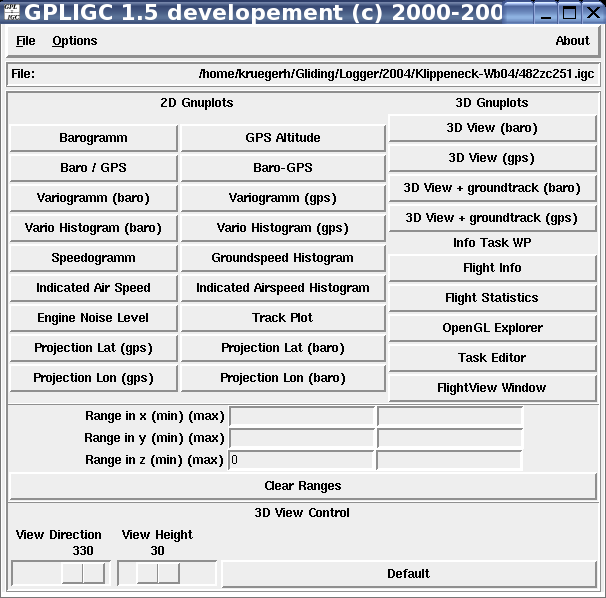
\includegraphics[width=\textwidth]{png/gpligc-main}
% \end{center}
% \end{figure}



\begin{figure}[h]
\caption{\label{flightview}The GPLIGC flight view window showing a flight with two tasks}
\begin{center}
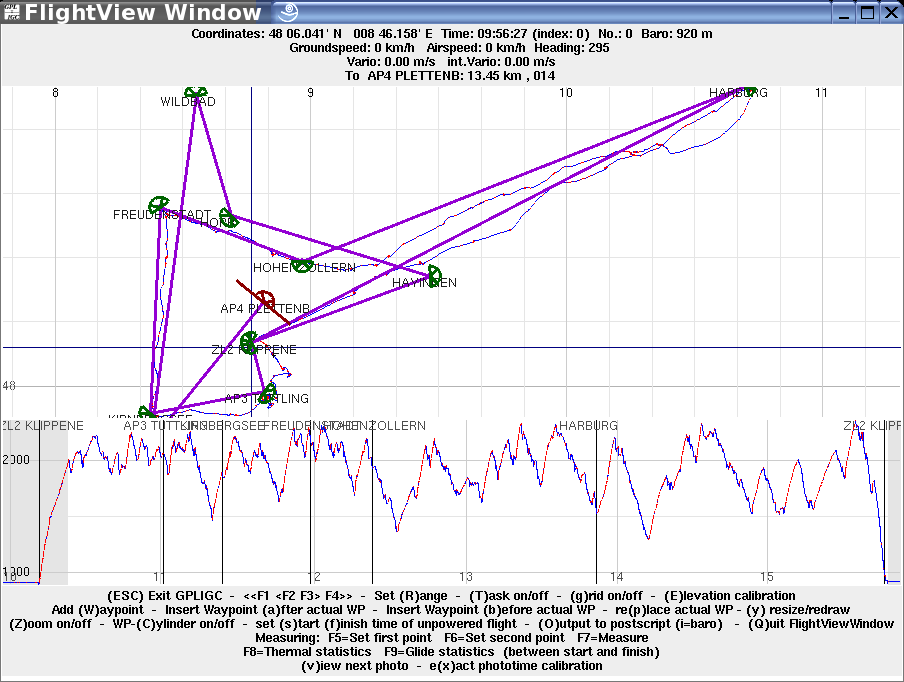
\includegraphics[width=\textwidth]{png/flightview-1}
\end{center}
\end{figure}

\begin{figure}[h]
\caption{\label{flightinfo}The GPLIGC flight info window}
\begin{center}
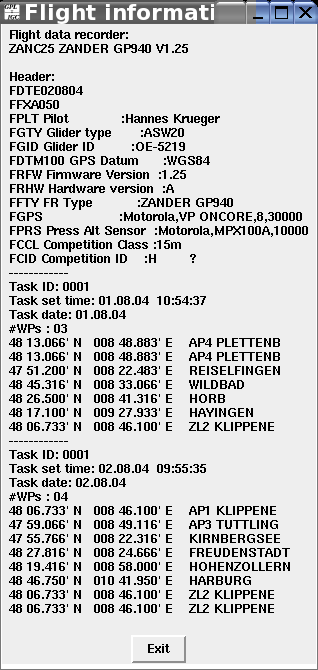
\includegraphics{png/flightinfo}
\end{center}
\end{figure}


\begin{figure}[h]
\caption{\label{taskeditor}The GPLIGC task editor window}
\begin{center}
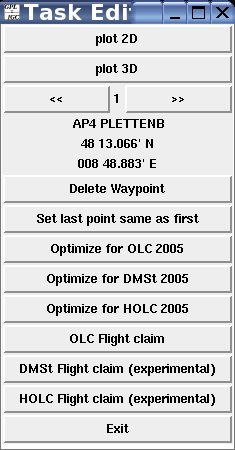
\includegraphics{png/taskeditor}
\end{center}
\end{figure}

\begin{figure}[h]
\caption{\label{flightview2}The GPLIGC flight view window, with the valid task}
\begin{center}
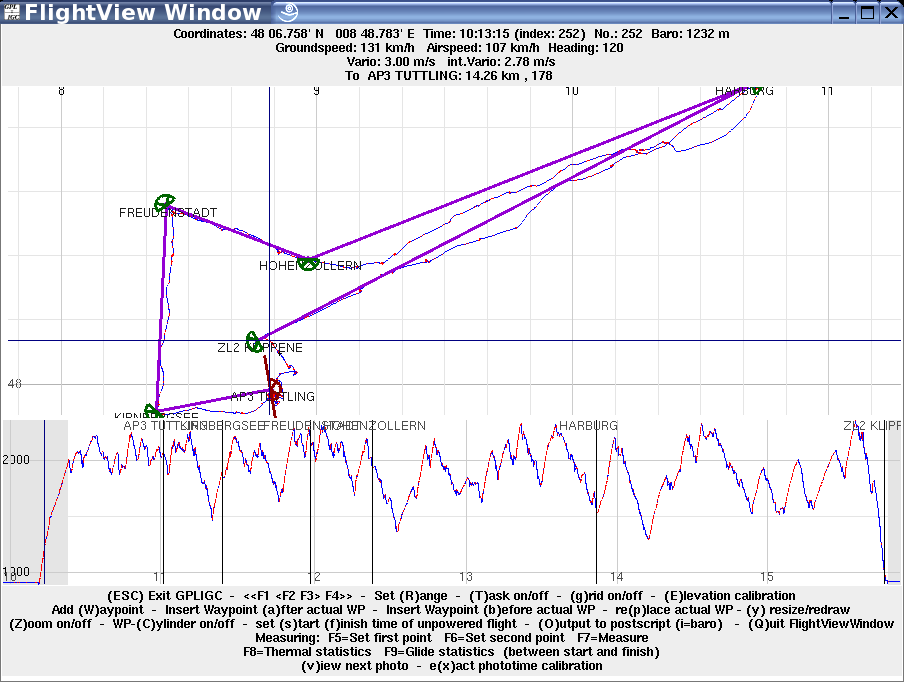
\includegraphics[width=\textwidth]{png/flightview-2}
\end{center}
\end{figure}

\begin{figure}[h]
\caption{\label{start}Crossing the starting line}
\begin{center}
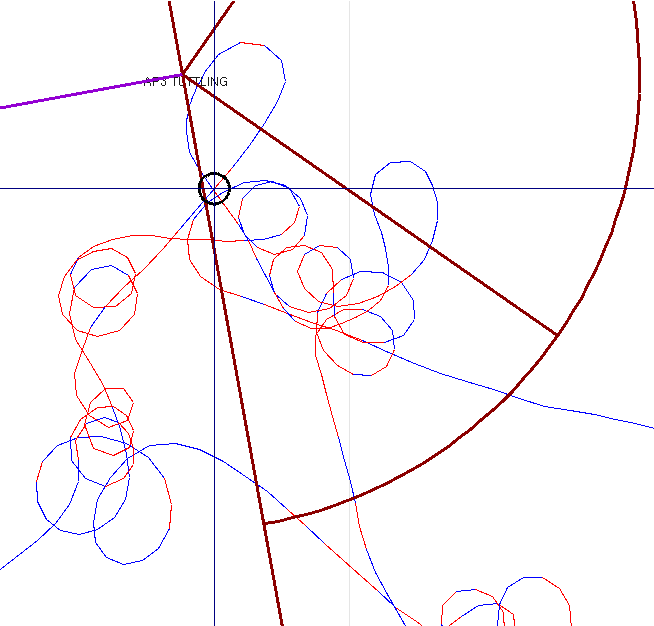
\includegraphics[width=\textwidth]{png/start}
\end{center}
\end{figure}

\begin{figure}[h]
\caption{\label{finish}Reaching the finishing line}
\begin{center}
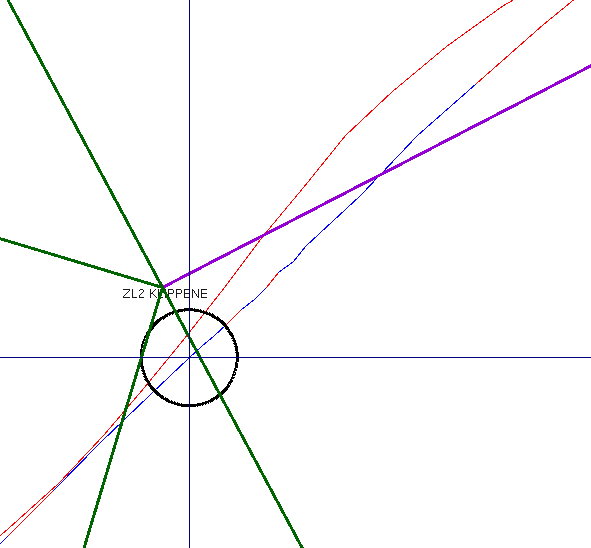
\includegraphics[width=\textwidth]{png/finish}
\end{center}
\end{figure}

\begin{figure}[h]
\caption{\label{flightstatistic}The GPLIGC flight statistic window}
\begin{center}
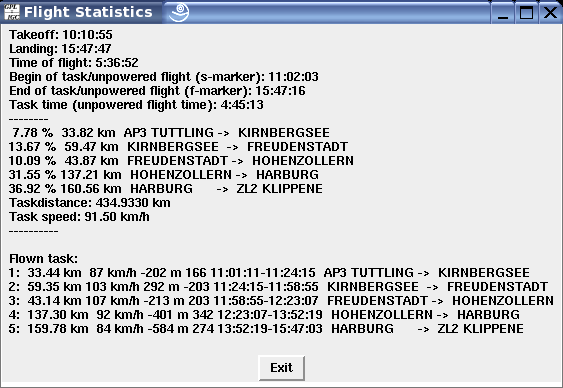
\includegraphics[width=\textwidth]{png/flightstatistic}
\end{center}
\end{figure}

\begin{figure}[h]
\caption{\label{thermals}The GPLIGC thermal statistics}
\begin{center}
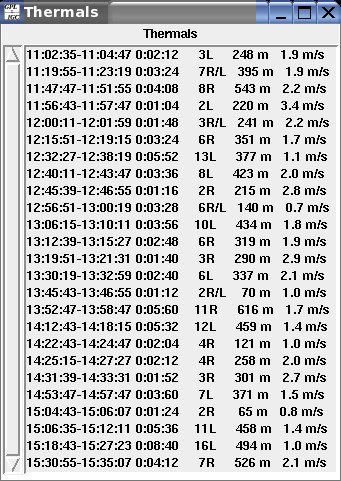
\includegraphics[height=13cm]{png/thermstat}
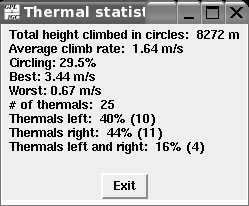
\includegraphics{png/thermstat2}
\end{center}
\end{figure}

\begin{figure}[h]
\caption{\label{glide}The GPLIGC glide statistics}
\begin{center}
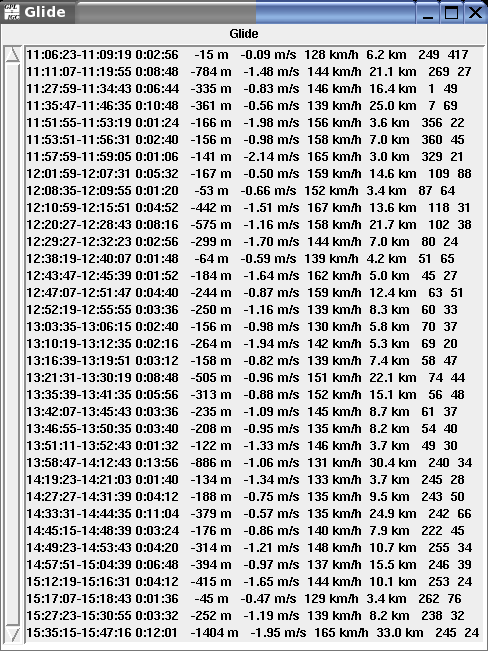
\includegraphics[height=13cm]{png/glidestat1}
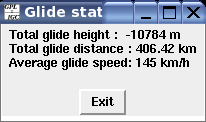
\includegraphics{png/glidestat2}
\end{center}
\end{figure}


\clearpage


\subsection{Innsbruck F\"ohn flight 2009-04-16-GAR-000-02.igc}

This nice example of a classical Innsbruck F\"ohn flight was done with our club DuoDiscus T in april 2009.

\subsubsection{Flight Information (additional)}
This tool allows us to enter/update some additional information. The date is shown correct, but the pilots name is missing.
Plane and callsign can be entered too, the QHN can be set to 1006 (if I remember right). The timezone is +2, and the airfield is Innsbruck (LOWI).

\subsubsection{Calibration of the altitude}
The track was recorded with a Garmin Geko 301.
Using the Flight View Window (fvw) the cursor can be set some point right before the take-off (e.g. 13:35).
As can be seen here, the recorded altitude is quite close to 580~m (which is the elevation of Innsbruck airport). The Geko's
auto calibration function did a good job (it corrects the reference pressure with averaged GPS altitudes).
Subsequently, the right elevation of Innsbruck LOWI (580~m) can be entered by pressing \keys{e}. If the \emph{save} button of the additional flight information tool is used, the calibration is saved and will be available later (after opening this file again). In this case the calibration is not really needed, since the offset is ca. three or four meters, only.

\subsubsection{Winch}
Using the fvw and the cursor (move with \keys{F1}--\keys{F4} or with the mouse), the winch take-off can be found between 13:35:26 and 13:36:05. To analyse the winch launch mark the first point with \keys{F5}, the second with \keys{F6}. Statistics is then calculated with \keys{F7}.
The launch took 42 seconds, the gain in altitude was 343~m with an average climbing rate of 8.2~m/s. The heading was 81$^\circ$, which is in good agreement with the runway 08. The speed of 91~km/h looks too small for a DuoDiscus, but the value reflects the projected groundspeed, not the airspeed. Change in altitude and the wind is not taken into account.

\subsubsection{Ridge soaring}
The lift at the ridge was entered at 13:36:38 and until 13:43:35 (within 7~min) 1700~m were gained in an average lift of 4.1~m/s with a nice maximum of ca. 8~m/s.

\subsubsection{Wave}
The first climb in the wave was found (after ATC clearence) at 13:56:20. In the following 10~min, ca.~1700m with an average of 2.8~m/s were climbed to the maximum of the ATC clearence. Subsequently airbrakes had to be used to limit the altitude.
As you can see in the barogram I really enjoyed beeing on top (for more than one hour). A feet heating device helped to stay warm at about -20$^\circ$C, and of course oxygen was used. Figure~\ref{foehngap} shows the view to the wave clouds and the typical foehn gap above the Inn valley.
The pictures are not included in the example, but the photo-locator option would look like Fig.~\ref{pic88}, showing the positions of the pictures. Btw. Fig.~\ref{pic88} was created using the postscript output from fvw via the keys \keys{o} and \keys{i}.

\begin{figure}[h]
\caption{\label{foehngap}Foehn gap and massive wave clouds above the Inn valley. The picture was taken in ca.~5000~m, the top of the Ac Len is probably higher than FL200.}
\begin{center}
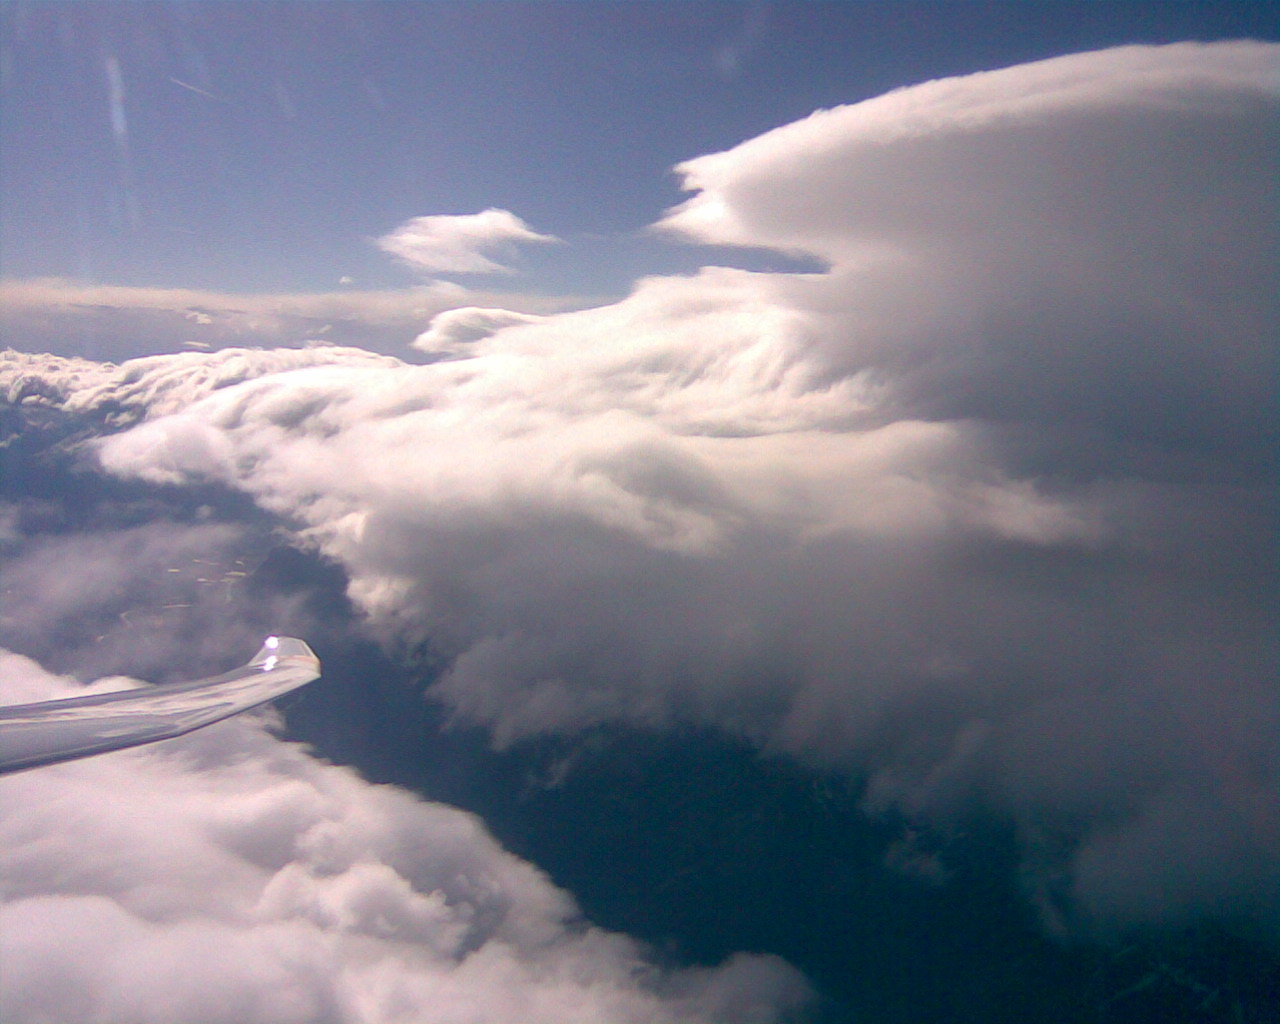
\includegraphics[width=\textwidth]{png/Bild088.jpg}
%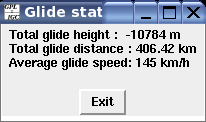
\includegraphics{png/glidestat2}
\end{center}
\end{figure}

\begin{figure}[h]
\caption{\label{pic88}Locating pictures}
\begin{center}
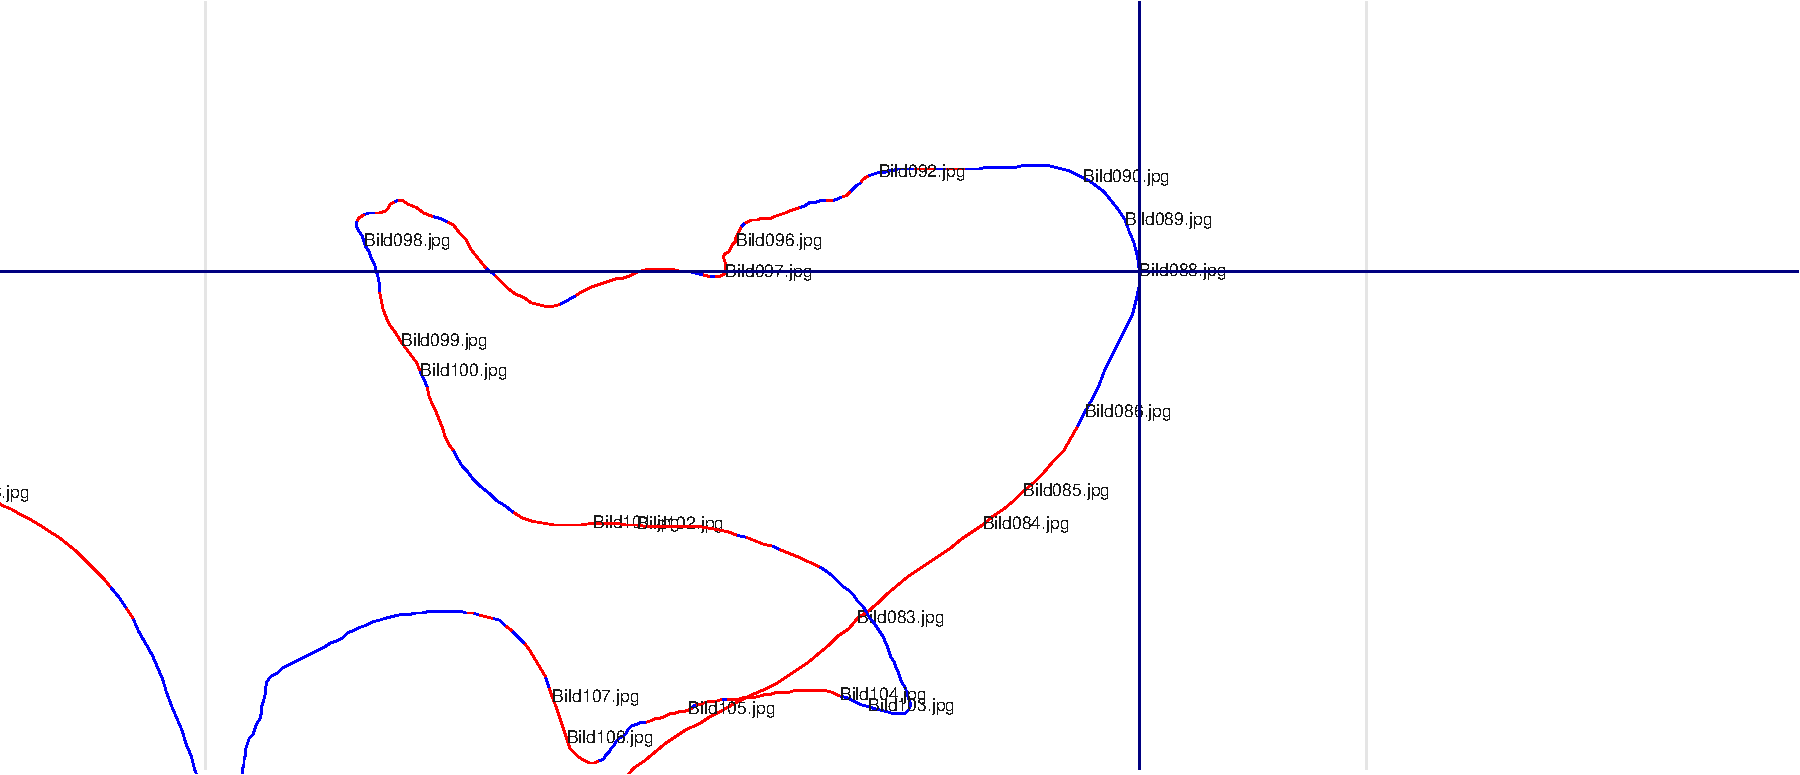
\includegraphics[width=\textwidth]{png/pic88fvw}
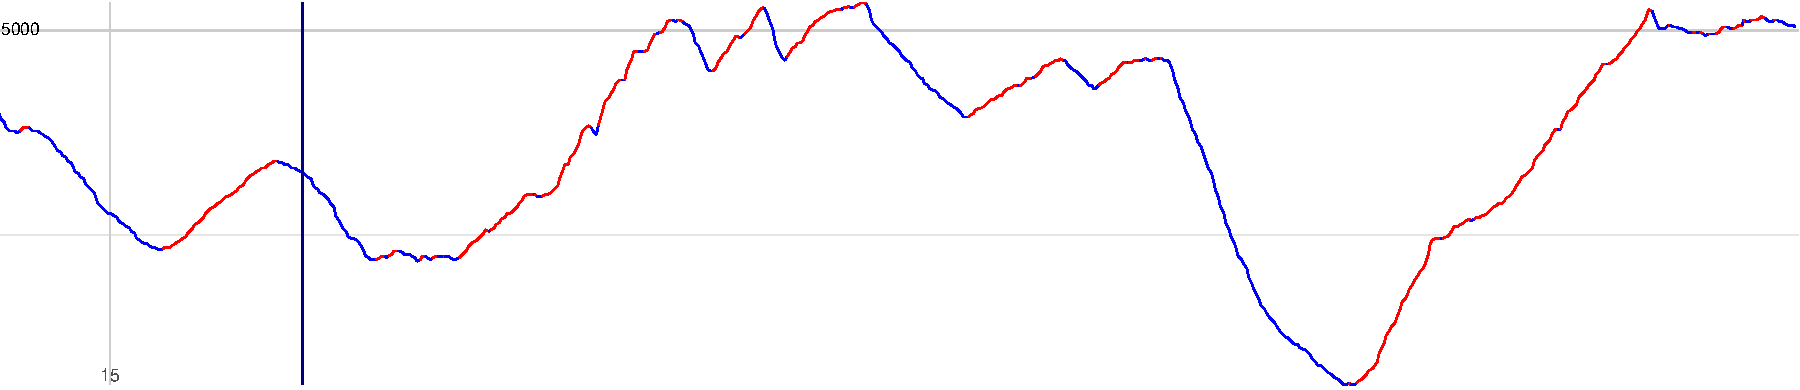
\includegraphics[width=\textwidth]{png/pic88fvwbaro}
\end{center}
\end{figure}


\subsubsection{Analysis of wind}
To analyse the wind, which causes such nice lifts, we have to select parts of the track including many different directions flown. Circling works very well, but some figure-of-eight turns can be used too.
13:36:29--13:39:35 corresponds to the first lift at the ridge up to ca.~1500m. Selecting this range (\keys{F5}/\keys{F6}) and pressing \keys{F7} will analyse the wind. The opened gnuplot window, shows how the groundspeed depends on the heading (if airspeed is recorded -- as e.g. in some Zander loggers -- the difference groundspeed-airspeed is used). A sinus function is fitted to the data, which gives the direction and speed of the wind. In this case its ca.~40km/h from 137$^\circ$. The direction is typical for this part of the Inn valley in foehn situations.

Another interesting part is from 14:06:29 to 14:18:53, which includes some circles and figure-of-eight turns in the wave just north of Nockspitze and Axamer Lizum. The analysis shows a wind from 190$^\circ$ with 50~km/h only, which is surprisingly low for such a strong wave.
The wave north of the Glungezer (14:25:14--14:56:32) shows a bit higher wind speed of 60~km/h and ca.~200$^\circ$.
The second ascend to the wave level (16:38:23--16:57:08) exhibits very similar wind conditions.

\subsubsection{Oxygen debriefing}
The \emph{Flight Statistics} window shows some information on (recommended) oxygen consumption. It is calculated for constant open-flow systems. The values in brackets corresponds to the use of an Oxymizer canula (ca.~1/3 of a regular open-flow system).
According to the FAR regulation 91.211 a total of 226~l of oxygen should have been used. Starting to use oxygen at FL100 (as recommended) would have increased the total to 275~l. Using an Oxymizer canula would have reduced these amounts to ca.~1/3.
However, modern pulse-demand systems save even more oxygen, depending on your breathing rate.


\clearpage

\subsection{using loopviewer.pl to make presentations of flights}

loopviewer.pl is a simple script, which uses ogie to show flights automatically.
This could be used for presentation of flights, e.g. at competitions.
loopviewer.pl reads a list, which contains two entries (enclosed in double quotes) per line:
the first is the path and name of the igc-file, the second a comment, which should be shown with the flight.
So far, this simple script needs manual editing, to obtain a reasonable set of parameters.


%\begin{enumerate}
%\item Step 1
%\item Step 2
%\item ...
%\end{enumerate}

\section{Tools}

This is a small collection of Perl scripts, which can be useful for GPLIGC and OGIE users.

\subsection{loopviewer.pl}
The \texttt{loopviewer.pl} is a small script which can be used as a template to create an automatic show of a list of igc files.
It is intended to be used at gliding competitions to have a nice presentation of all flights. All pilots can enjoy every flight of the day, while having a nice cold beer in the briefing hangar (video-beamer!).
Therefore a list has to be created containing one line for every flight. Each line should contain the quoted path to the igc-file and a quoted information string: \\
\texttt{"c:$\backslash$path$\backslash$to$\backslash$file.igc"   "1. - Name - ASW20 - II - 610.34km - 102.3km/h - 1000pts"} \\
\texttt{"c:$\backslash$path$\backslash$to$\backslash$file2.igc"  "2. - Name - Ventus2 - I2 - 610.34km - 101.7km/h - 980pts"} \\
\texttt{...} \\
The configuration file should be set up to have some nice maps from the contest area, airspaces and whatever is needed. A good initial viewpoint position should be determined in some interactive run, subsequently the corresponding options can be changed in the \texttt{loopviewer.pl} script, which can be started with this simple call: \\
\texttt{loopviewer.pl  list} \\
where \texttt{list} is the file containing the above mentioned list.


\subsection{Garmin related tools}

Since I bought a Garmin Geko301, a few tools have been developed to use the Garmin's track logs etc.

I recommend to use \emph{gpspoint}  by Thomas Schank to do the data transfers to and from your Garmin device.
To handle the output from \emph{gpspoint} the following tools can be used.

\subsubsection{gpsp2igc.pl and gpsp2igcfile.pl}
\label{gpsp2igc}
This tool can convert the track log output from \emph{gpspoint} (\texttt{gpspoint -dt >tracklog.gpsp})
to something like an igc-file to be read by GPLIGC \& OGIE.

I use gpspoint as follows:

\texttt{gpspoint -p /dev/ttyS0 -dt | gpsp2igc.pl >out.igc}

gpsp2igcfile.pl creates IGC-file(s) with a filename corresponding to the date(s) of the recording.



\begin{appendix}

%$Id: gpligc_config.tex 3 2014-07-31 09:59:20Z kruegerh $
%;;; Local IspellDict: "british"


\section{The .gpligcrc configuration file}
\label{gpligcrc}
The \emph{GPLIGC} configuration file.
The keys and values in this configurationfile are \emph{case-sensitive!}.

The following list contains the config-keywords with default values and (for some)
a short description including valid alternative values.

%\textbf{Windows}: on windows platforms this file is named \texttt{gpligc.ini}

\begin{itemize}

\item \texttt{DEBUG    "0"} \\
 This should be set to "1" for debugging purposes.

\item \texttt{ENL\_noise\_limit    "500"}
\item \texttt{altitude\_unit\_factor    "1"}
\item \texttt{altitude\_unit\_name    "m"}
\item \texttt{baro\_grid\_large    "1000"} \\
 This changes the spacings of the gridlines in the barograph in the flight-view-window
\item \texttt{baro\_grid\_small    "500"}
\item \texttt{baro\_histo\_intervall    "50"}\\
    Interval for the altitude histograms in m
\item \texttt{browser    "/usr/local/mozilla/mozilla"}\\
 Select your favourite browser here.
\item \texttt{coordinate\_print\_format    "igch"}
\item \texttt{cylinder\_linewidth    "3"}
\item \texttt{distance\_unit\_factor    "1"}
\item \texttt{distance\_unit\_name    "km"}
\item \texttt{draw\_task "1"} \\
defines, whether the task is drawn by default in flight-view-window (1) or not (0)
\item \texttt{draw\_wpcyl "1"}\\
defines, whether waypoint cylinders/sectors are drawn by default in flight-view-window (1) or not (0)
\item \texttt{fvw\_grid    "yes"}

\item \texttt{fvw\_baro\_grid    "yes"}

%not used any longer
%\item \texttt{fvw\_show\_help "1"}\\
%Setting this to 0 will stop showing the help in fvw. Saves quite a bit of space.


\item \texttt{fvw\_baro\_fraction "3"}\\
This determines, how large the barogramm area is compared to the track area (in fvw).
3 would result in 1/3. (the larger the number, the smaller the barogramm). Allowed values 1.1--10.
Given number does not need to be an integer.

\item \texttt{garmin\_download    "sudo gpspoint -dt -p /dev/ttyUSB2"} \\
this command is used to download tracks from a GPS device.

\item \texttt{geotag\_force\_overwrite    "0"} \\
  by default (value 0) GPS tags in the exifdata are not overwritten. If set to 1, the geotag feature will
overwrite existing GPS tags in images (without further notice!).

\item \texttt{gnuplot\_4\_terminal    "0"} \\
 In case of "1" an additional gnuplot shell will be started for each gnu-plot
\item \texttt{gnuplot\_draw\_style    "with lines"}
\item \texttt{gnuplot\_grid\_state    "set grid"}
\item \texttt{gnuplot\_major\_version    "4"}
\item \texttt{gnuplot\_terminal    "x11"}
\item \texttt{gnuplot\_terminal\_app    "xterm -e"}\\
    The terminal application to be used for the gnuplot shell
\item \texttt{gnuplot\_win\_exec    "wgnuplot.exe"}\\
    Contains the filename of the gnuplot-binary on Windows platforms

\item \texttt{gpsbabel\_tdownload  "sudo gpsbabel -t -i garmin -f /dev/ttyUSB2 -o igc -F "}\\
  contains the command string to be used to download trackdata via \emph{gpsbabel}~\cite{gpsbabel}. The last option should be -F, since the output file name will be appended to this string.

\item \texttt{integrate\_over    "10"}\\
    Some of the data plots use integrated values. This will define how many data-points will
    be used for  integration
\item \texttt{libdir    "/usr/local/share/gpligc/"}\\
    The path which will be used to load the library-files

\item \texttt{map\_max\_tiles "30"}\\ Maximum number of tiles used on the screen (default 30). If this is exceeded the next smaller zoom level will be used.
\item \texttt{map\_max\_scalesize "750"}\\ Maximal dimension for ``upscaling`` maptiles (default 750).
If map tiles would be scaled beyond this limit, the next higher zoom level is used.
\item \texttt{maps\_zoomlevel "8"}\\ The default map zoom-level (recommended: 8).
\item \texttt{maps "1"}\\ can be 0 or 1. default behaviour maps on/off.
\item \texttt{map\_path "HOME/.gpligc/map"}\\
default directory for maps. Default value depends on the platform.
%Windows: c:\textbackslash GPLIGC\textbackslash map, unix: HOME/.gpligc/map.
If an environment variable GPLIGCHOME is set, a "map" directory will be created within GPLIGCHOME.

\item \texttt{map\_type "osm"}\\  osm=openstreetmap


\item \texttt{marker\_linewidth    "3"}
\item \texttt{mm\_download\_dirs    "Aufnahmen Fotos Videoclips"}\\
	Directories, from where (multimedia) files will be copied (see mm\_mountpoint too)
\item \texttt{mm\_mountpoint    "/mnt/sdC"} \\
	Mountpoint for your multimedia recorder (e.g. mobile phone). Should be user mountable.
\item \texttt{mm\_player    "mplayer"} \\
	Player to be used for multimedia files (audio recordings, movies, etc)

\item \texttt{new\_version\_message\_shown    "0.1"}

\item \texttt{open\_additional\_info    "0"}\\
    If set to 1, the ``additional info dialog'' is opened immediately in cases where no gpi-file is found.

% pre 1.10
% \item \texttt{open\_flight\_view\_window    "1"}\\
%     The flight-view-window will be opened for each igc file opened if set to 1.

\item \texttt{optimizer\_cycles\_mmc    "20"} \\
	For all of the \texttt{optimizer\_*} keys see section~\ref{optimise}
\item \texttt{optimizer\_cycles\_sa    "5"}
\item \texttt{optimizer\_debug    "0"}
\item \texttt{optimizer\_method    "mmc"}
\item \texttt{optimizer\_mmc    " -m 1000 -mmc 25000 -devisor 3 -refine 2 "}
\item \texttt{optimizer\_sa    " -sima -m 1000 -sacycles 500 -saexp -sapara 15.0 -saparb 0.03 -devisor 3 -refine 2 "}
\item \texttt{optimizer\_verbose    "0"}


\item \texttt{photo\_path    "none"}
\item \texttt{photos    "1"}
\item \texttt{picture\_viewer    "internal"}\\
    Whether to use the "internal" or any other picture viewer. My favourite is "kuickshow"
\item \texttt{skip\_check    "1"}\\
    With "1" a skip-check is performed. If the difference between to logged positions is larger than
    skip\_limit\_minutes the skip will be marked.
\item \texttt{skip\_del\_first\_after    "1"} \\
	This circumvents a bug in the Garmin Geko tracklogs. The first position fix after a skip will be discarded.
\item \texttt{skip\_limit\_minutes    "0.2"}\\
    Limit to detect skips in the tracklog
\item \texttt{speed\_histo\_intervall    "5"}\\
    Interval for the speed histogram in km/h
\item \texttt{speed\_unit\_factor    "1"}
\item \texttt{speed\_unit\_name    "km/h"}
\item \texttt{task\_linewidth    "3"}
\item \texttt{terminal    "xterm -hold -e"} \\
	terminal application to be used for some things (copying Multimedia files, downloading from Garmin)

\item \texttt{te\_vario\_fallback "0"}\\
The total energy compensated vario is usually calculated from the airspeed. Since many loggers dont log airspeed,
the total energy compensation can be calculated from groundspeed (errors can be large in case of significant wind).

\item \texttt{te\_warning    "1"}\\
A warning on groundspeed total energy compensation can be disabled setting this to 0.

\item \texttt{terminal	"xterm -hold -e"}\\
Terminal command used for download of garmin-tracks and media

\item \texttt{timezone    "0"}\\
Offset to local timezone (e.g. timezone used in your camera) . Used for the photo locator.

\item \texttt{vario\_histo\_intervall    "0.5"}\\
    Interval for the vertical speed histograms in m/s
\item \texttt{vertical\_speed\_unit\_factor    "1"}
\item \texttt{vertical\_speed\_unit\_name    "m/s"}

\item \texttt{viewclick\_res "1"}\\
	If you experience serious delays in moving the crossmarks in the fvw by clicking close to the track, you may increase this number to a larger integer

\item \texttt{waypoint\_linewidth    "3"}
\item \texttt{wind\_analysis "1"} \\
If set to "1", a airspeed-groundspeed difference is plottet with F5/F6/F7 statistics.

\item \texttt{window\_height "500"} \\
\item \texttt{window\_width "900"} \\
size of the plotting area of the main window (pixels)


\item \texttt{working\_directory    "/home/user1/IGC"}
\item \texttt{zoom\_sidelength    "10"}\\
    Sidelength of the zoom-window in km
\item \texttt{zylinder\_names    "1"}
\item \texttt{zylinder\_radius    "500m"}
\item \texttt{zylinder\_wp\_type    "both"}

\end{itemize}

%%% Local Variables:
%%% mode: latex
%%% TeX-master: "GPLIGC_manual.tex"
%%% End:

\newenvironment{hkkeys}
    {\begin{list}{}
        {
        \setlength{\leftmargin}{9em}
        \setlength{\labelwidth}{8em}
        \setlength{\labelsep}{2em}
        \setlength{\parsep}{0em}
        \setlength{\itemsep}{0.5ex}
        }
    }
    {\end{list}}


\section{OGIE keyboard control}
\label{keys}

The keys are case sensitive.

\subsection*{Movement}

\begin{hkkeys}
\item[\keys{a}]        fast backward
\item[\keys{s}]        backward
\item[\keys{g}]        forward
\item[\keys{space}]    fast forward
\item[\keys{d}]        left
\item[\keys{f}]        right
\item[\keys{t}]        up
\item[\keys{z}]        down
\item[\keys{q}, \keys{esc}]    escape
\item[\keys{\arrowkeyleft}, \keys{\arrowkeyright}] rotation around marker
\item[\keys{\arrowkeyup}, \keys{\arrowkeydown}] rotation around marker
\item[\keys{\shift+\arrowkeyleft}, \keys{\shift+\arrowkeyright}]
            rotation around center
\item[\keys{\shift+\arrowkeyup}, \keys{\shift+\arrowkeydown}]
            rotation around center

\end{hkkeys}



\subsection*{Viewing modes}

\begin{hkkeys}
\item[\keys{l}]        terrain on/off (build up from DEM data)
\item[\keys{L}]        wireframe mode on/off
\item[\keys{b}]        maps on/off (if texture maps specified in config-file)
\item[\keys{x}, \keys{c}] 	switch to previous/next map-set
\item[\keys{w}]        fullscreen on/off
\item[\keys{o}]        switch 2D-ortho/3D-perspective view mode
\item[\keys{h}]        curtain on/off
\item[\keys{B}]        toggle Grayscale/Color-mode

\item[\keys{1}]  max's special colormap
\item[\keys{2}]  atlas colormap
\item[\keys{3}]  single color (gray-ramp)
\item[\keys{4}]  dark green $\rightarrow$ yellow $\rightarrow$ red
\item[\keys{5}]  magenta $\rightarrow$ dark blue $\rightarrow$ turquois
\item[\keys{6}]  black $\rightarrow$ rainbow $\rightarrow$ white

\item[\keys{F10}, \keys{F11}] decrease, increase number of lower colormap

\item[\keys{\shift+F5}, \keys{\shift+F6}]
        switch flight linestrip mode: up/down, altitude, speed, vario

\item[\keys{\shift+F7}, \keys{\shift+F8}]
        decrease, increase colormap applied to flight linestrip

\item[\keys{\shift+F3}, \keys{\shift+F4}]
        decreas, increase Fligh linestrip width (1-5)



\item[\keys{O}]        flat shading on/off
\item[\keys{j}]        fog on/off
\item[\keys{9}, \keys{0}]      decrease, increase fog-density
\item[\keys{7}, \keys{8}]      decrease, increase field-of-view-angle

\item[\keys{{+}}, \keys{--}]      increase, decrease z-axis scaling

\item[\keys{F5}]       Reset Viewpoint to initial position
\item[\keys{F6}]       Info on/off

\item[\keys{M}]        Lock position relative to marker (follow-mode)
\item[\keys{U}]        Display a part of the flight only  on/off
\item[\keys{I}]        Move Marker automatically forward... (Movie-Mode)
\item[\keys{J}]        Turn joystick on/off

\item[\keys{\shift+F1}, \keys{\shift+F2}]
        decrease, increase framerepeat  in moviemode. Use to slow down animation.

\item[\keys{F8}]       Modulate (texture maps with coloured surface elevation) on/off
\item[\keys{F9}]       Airspace on/off
\item[\keys{\shift+F9}] Airspace wireframe mode on/off
\end{hkkeys}


\subsection*{Marker}

\begin{hkkeys}
\item[\keys{F1}]       marker fast backward
\item[\keys{F2}]       marker backward
\item[\keys{F3}]       marker forward
\item[\keys{F4}]       marker fast forward
\item[\keys{F7}]       Marker on/off
\item[\keys{page-up}]  increase size of marker
\item[\keys{page-down}] decrease size of marker
\end{hkkeys}


\subsection*{Other options}

\begin{hkkeys}
\item[\keys{m}]        mouse control on/off
\item[\keys{p}]        screenshot (jpeg's are written as frameNUMBER.jpg)
        with NUMBER starts at 0000 each session.

\item[\keys{P}]        continous screenshots
        (each rendered frame will be saved as jpeg).

\item[\keys{y}]        texture map compression on/off (on supported systems)

\item[\keys{u}, \keys{i}]      increase, decrease elevation offset
        (shifts flight against terrain)
\end{hkkeys}


\subsection*{Lifts}
\begin{hkkeys}
\item[\keys{\shift+page-up}] increases text size
\item[\keys{\shift+page-down}] decreases text size
\item[\keys{Pos1}] switches info up
\item[\keys{End}] switches info down
\end{hkkeys}

\subsection*{Waypoints}
\begin{hkkeys}
\item[\keys{F12}] showing waypoints on/off
\item[\keys{\shift+page-up}] increases text size
\item[\keys{\shift+page-down}] decreases text size
\item[\keys{\shift+Pos1}] switches info up
\item[\keys{\shift+End}] switches info down
\end{hkkeys}


\subsection*{Stereoscopic view modes}

\begin{hkkeys}
\item[\keys{S}]        stereoscopic double-image
\item[\keys{D}]        Red-Green stereoscopic
\item[\keys{F}]        Red-Blue stereoscopic
\item[\keys{A}]        swap images (right/left)
\item[\keys{Q}]        decrease eye distance by 50m
\item[\keys{W}]        increase eye distance by 50m
\end{hkkeys}

%$Id: explorer_cmdline.tex 3 2014-07-31 09:59:20Z kruegerh $
%;;; Local IspellDict: "british"


\section{Commandline options (OGIE)}
\label{cmdline}

\emph{OGIE} has a lot of commandline options. For a full list try:\\
\texttt{ogie --help} \\
Commandline arguments override configuration file settings, which override
compiled-in-defaults. For most options there is an option to turn the feature on, and another option to turn it off, so you are able to override all
possible configuration file settings. 
Many of the options can be changed at runtime via keyboard input or menus, but some are \emph{start-time-options}, which can be activated or set at the time the program is started, only.
These are marked (ST).

Options marked as \emph{default} are active by default (compiled in). This may be overridden by the configuration-file, or commandline switches.

Some of the commandline-switches (or commandline-options) require  additional parameters (\texttt{INT, FLOAT, FILE} or \texttt{STRING}), the meaning of these can be read in section \ref{config}.

\subsection{All available commandline options}

\begin{itemize}

\item \texttt{-h, --help} \\
Print help and all available commandline options (ST)

\item \texttt{-V, --version} \\
Print version information (ST)

\item \texttt{-v, --verbose} \\
Be verbose, lots of console output (ST)

\item \texttt{--quiet} \\
Turn off verbosity no output to console. Overrides --verbose and VERBOSE (ST)

\item \texttt{-q, --query-gl} \\
Querying openGL implementation. This will give out some information about your specific OpenGL implementation (ST)

\item \texttt{--check} \\
This returns exitcode 0. Used by GPLIGC to check if OGIE is available (ST)

\item \texttt{--debug} \\
This overrides --verbose and --quiet. Lots of ugly debugging output (ST).

\item \texttt{--compiler} \\
This will give out some information about compiler and building environment (ST)

\item \texttt{-i FILE, --igc-file=FILE} \\
This option specifies the igc-file to be opened (ST)

\item \texttt{--gpsd} \\
Try to connect to local gpsd, retrieve position data, and start in live-mode (ST).
Ogie has to be compiled with gpsd support (See section \ref{unix_install}).

\item \texttt{--gpsd-server=STRING} \\
network address of gpsd server (ST)

\item \texttt{--gpsd-port=INT} \\
port number of gpsd server (ST)


\item \texttt{-g, --gpsalt} \\
The altitude from GPS will be used instead of barometric (ST)

\item \texttt{-b, --baroalt} \\
Barometric altitude will be used (default, ST)

\item \texttt{--use-all-fixes} \\
Use all position fixes. Even those which are flagged invalid. (ST)

\item \texttt{--lat=FLOAT} \\
Latitude of centre. Used for terrain viewing without igc-file (ST)

\item \texttt{--lon=FLOAT} \\
Longitude of centre. Used for terrain viewing without igc-file (ST)

\item \texttt{--get-elevation} \\
To be used with --lat and --lon. Will return the elevation of the given coordinates,
if a DEM is configured. To be used with SRTM-3 data. (elevation=0 is the void-flag, at least in the usgs seamless server downloads).
INVALIDn is returned, if n neighbouring grid-points are invalid. n=9 is returned, if the requested
position is not covered by the configured DEM.
The second value which is returned is the max difference in elevation of the four neighbouring grid-points, the maximum of the remaining
neighbours for INVALID1-3, 0 for INVALID4 and 9999 for INVALID9. (ST)


\item \texttt{-c FILE, --config-file=FILE} \\
Used to open a non-standard config file (ST)

\item \texttt{-o, --ortho} \\
Forces startup in 2D orthographic viewing mode

\item \texttt{--perspective} \\
Forces startup in  3D viewing mode

\item \texttt{--aov=INT} \\
This sets the angle of view (1-179)

\item \texttt{-l, --landscape} \\
Use digital elevation data to display terrain

\item \texttt{-f, --flat} \\
Don't use terrain from DEM. Use flat surface instead

\item \texttt{-m, --map} \\
Activates displaying of digitised maps. If configured in configuration file.

\item \texttt{--no-map} \\
Don't use digitised maps

\item \texttt{--map-set-name=STRING} \\
Name of map set to use as default

\item \texttt{--modulate} \\
Maps are coloured by DEM altitude colour, if this option is active

\item \texttt{--no-modulate} \\
Use original colour of maps

\item \texttt{--maps-unlighted} \\
If maps used with DEM and \texttt{--no-modulate}, this turns off lighting of the maps (ST)

\item \texttt{--maps-lighted} \\
Maps are lighted, if used with DEM and no modulation. (Default behaviour) (ST)

\item \texttt{--no-lighting} \\
Don't use lighting. Use for orthomode with upscaling recommended (ST)

\item \texttt{--terrain-shading} \\
Terrain shading. This implies the \texttt{--no-lighting} option (ST)

\item \texttt{--shading-scale=FLOAT} \\
Strength of terrain shading. The smaller the value, the stronger the effect.
If not given, the max elevation difference divided by seven is used (ST)

\item \texttt{--light-direction=INT} \\
The direction of the light for terrain shading. 1 corresponds to north, 2 nort-east, 3 east, 4 south-east, 5 south,
6 south-west, 7 west, 8 north-west (ST)

\item \texttt{-a, --airspace} \\
Turn on airspace visualisation

\item \texttt{--no-airspace} \\
Turn off airspace visualisation

\item \texttt{--airspace-wire} \\
Turn on airspaces in wireframe mode

\item \texttt{--airspace-wire-col-[r|g|b]} \\
Defines colours for airspace wireframe lines

\item \texttt{--airspace-wire-width}\\
Sets the linewidth used to draw airspace wireframes.

\item \texttt{--airspace-transparent} \\
Turn on transparent airspace.

\item \texttt{--airspace-limit=INT} \\
Airspaces, which lower boundary is higher that this limit (in FL), will not be shown. (ST)

\item \texttt{--airspace-file=FILE} \\
Use airspaces from file (OpenAir\texttrademark -format) (ST)

\item \texttt{-w, --wire} \\
Draw terrain surface as wireframe-model

\item \texttt{--filled} \\
Use filled polygons for terrain (default)

\item \texttt{--grayscale} \\
Use gray scaled image

\item \texttt{--color} \\
Use coloured image (default)

\item \texttt{--stereo} \\
Use double image stereoscopic mode

\item \texttt{--no-stereo} \\
Do not use stereoscopic modes (default)

\item \texttt{--stereo-rg} \\
Use anaglyphic stereoscopic mode (red/green)

\item \texttt{--no-stereo-rg} \\
Do not use anaglyphic stereoscopic mode red/green (default)

\item \texttt{--stereo-rb} \\
Use anaglyphic stereoscopic red/blue mode

\item \texttt{--no-stereo-rb} \\
Do not use anaglyphic stereoscopic red/blue (default)

\item \texttt{--stereo-hw} \\
Use stereoscopic hardware if available (ST)

\item \texttt{--no-stereo-hw} \\
Do not use stereoscopic hardware (default)

\item \texttt{--inverse-stereo} \\
Swap right/left image for stereoscopic modes

\item \texttt{--no-inverse-stereo} \\
Don't swap images right/left (default)

\item \texttt{--eye-dist=FLOAT} \\
Set eye distance for stereoscopic viewing modes (default=0.2km)

\item \texttt{--flat-shading} \\
Do not use gouraud shading (every triangle of the surface will get the same colour)

\item \texttt{--gouraud-shading} \\
Use gouraud-shading (default)

\item \texttt{--quads}\\
Use quadrilaterals to build terrain surface (ST)

\item \texttt{--curtain} \\
Draw curtain (default)

\item \texttt{--no-curtain} \\
Do not draw curtain

\item \texttt{--haze} \\
Enable atmospheric haze

\item \texttt{--no-haze} \\
Do not use atmospheric  haze (default)

\item \texttt{--haze-density=FLOAT} \\
haze density (0.0 clear - 0.5 dense fog)

\item \texttt{--colormap=INT} \\
Use colourmap \texttt{INT} for terrain surface (see \ref{color})

\item \texttt{--colormap-sea=INT} \\
Use colourmap \texttt{INT} for seafloor (see \ref{color})

\item \texttt{--colormap-min=INT} \\
Minimum altitude for colour scale (ST)

\item \texttt{--colormap-max=INT} \\
Maximum altitude for colour scale (ST)

\item \texttt{--sealevel=INT} \\
Elevation of sealevel. Beneath this elevation seafloor colourmap is used, above terrain colourmap (ST)

\item \texttt{--sealevel2=INT} \\
Elevation of sealevel2. The blue ocean will be drawn at elevation of sealevel2 (ST)

\item \texttt{--sealevel3=INT} \\
Elevation of sealevel3. A transparent blue surface will be drawn at elevation of sealevel3 (ST)

\item \texttt{--ignore-elev-[min,max]=INT} \\
Defines limits or a range, which are not used for determining the extrem values of the topography (ST)

\item \texttt{-s FLOAT, --scalez=FLOAT} \\
Z-axis scaling. A factor of 1.0 represents the \emph{real} relations. A default value of 3.0 is used to emphasise altitude

\item \texttt{-d INT, --downscaling=INT} \\
DEM raster downscaling can be used to reduce resolution of surface (to show larger areas) (ST)

\item \texttt{--upscaling INT}
The resolution of the DEM raster is enhanced by interpolation. Use with care,  higher factors increase the number of
triangles used dramatically. Good for small area terrain display (ST)

\item \texttt{--fullscreen} \\
Start up in fullscreen mode

\item \texttt{--window} \\
Start windowed (not fullscreen, default)

\item \texttt{--width=INT} \\
Set initial width of window (pixels)

\item \texttt{--height=INT } \\
Set initial height of window (pixels)

\item \texttt{--border=FLOAT } \\
Adds a \texttt{FLOAT} km border at top, bottom, right and left margin (ST)

\item \texttt{--border-lat=FLOAT} \\
Adds a \texttt{FLOAT} km border at top and bottom margin (ST)

\item \texttt{--border-lon=FLOAT} \\
Adds a \texttt{FLOAT} km border at right and left margin (ST)

\item \texttt{--offset=INT} \\
Shifts the flight \texttt{INT} meters up (relative to the dem surface)

\item \texttt{-e INT, --airfield-elevation=INT} \\
Sets the elevation of the take-off location (in m). The relative shift of the flight will be calculated automatically

\item \texttt{--marker-pos=INT } \\
Set the position of the marker to datapoint number \texttt{INT}

\item \texttt{--marker-time=string } \\
Set the position of the marker to datapoint nearest to HH:MM:SS

\item \texttt{--marker } \\
Activated the marker at start-time

\item \texttt{--marker-size=FLOAT}\\
Size of the Marker (0.01-10)

\item \texttt{--no-marker} \\
Disables marker at start-time (default)

\item \texttt{--info} \\
Activates info text display at start-time

\item \texttt{--no-info} \\
Turns the info text display off (default)

\item \texttt{--text="STRING"} \\
With this option a text string can be specified, which will be displayed
in the first line of the info text (ST)

\item \texttt{--no-position-info}\\
This option removes the information about the viewpoint position.

\item \texttt{--no-marker-pos-info}\\
To turn off the information about the marker position use this option.

\item \texttt{--text-size=FLOAT}\\
Size of text for points/lifts (0.001-1.0)

\item \texttt{--text-width=FLOAT}\\Width of text (1-20)

\item \texttt{--lifts=STRING}\\GPLIGC liftsfile (ST)

\item \texttt{--lifts-info-mode=INT}\\which info to display (1= int. vertical speed, 2=verical speed, 3=altitude, 4=time, 5=time, 6=date, 7=file)


\item \texttt{--waypoints-file=STRING}\\
  set the waypointsfile (see~\ref{wp}). Overrides any names given in the config file
\item \texttt{--waypoints}\\
	show waypoints  (default=off)
\item \texttt{--no-waypoints}\\
        dont show waypoints  (default=off)
\item \texttt{--waypoints-info-mode=INT}\\
	sets info to display (1-4: 1=description, 2=name, 3=altitude [m], 4=symbol).

\item \texttt{--waypoints-offset=INT}\\
        draw the text for the waypoints INT m higher that their actual elevation. Useful mountenous terrain. Default=300. If you want the waypoint spheres drawn higher too, you may set WAYPOINTS\_OFFSET\_TEXT\_ONLY to false (see~\ref{config}) or use \texttt{--waypoints-offset-spheres}.

\item \texttt{--waypoints-offset-spheres=INT}\\
        draw the text and spheres for the waypoints INT m higher that their actual elevation. Useful mountenous terrain.

\item \texttt{--flighttrack-mode=INT}\\
Sets the mode of track display. The interger value can be one of 0,1,2 or 3. 0: Classic mode, two colours (climbing, descending), colours can
be changed with \texttt{FLIGHTSTRIPCOL[UP|DOWN]\_[R|G|B]}. 1: Colour gradient (see \texttt{--flighttrack-colormap}) is used to display altitude
(this is the default).
2: Colour gradient is used to show speed. 3: Colour ramp is used to show vertical speed.

\item \texttt{--flighttrack-colormap=INT}\\
Sets the colourmap used to display the flighttrack. Integers from 1 to 7 can be used (see \ref{color}).

\item \texttt{--flighttrack-linewidth=FLOAT}\\
Sets the linewidth of the flighttrack. Floating point values in the range of 1.0 -- 5.0 can be used.

\item \texttt{--follow} \\
The viewpoint will be coupled with marker (default)

\item \texttt{--no-follow} \\
Makes viewpoint independent of marker position

\item \texttt{--marker-range} \\
A range (in time; future-past) around marker is plotted only

\item \texttt{--no-marker-range} \\
Full flight data is displayed (default)

\item \texttt{--marker-ahead=INT} \\
Defines marker range (datapoints in future of marker position) (ST)

\item \texttt{--marker-back=INT} \\
Defines marker range (datapoints in the past of marker position) (ST)

\item \texttt{--movie} \\
This will start up ogie in movie mode.

\item \texttt{--cycles=INT} \\
If given, ogie will perform INT cycles in movie mode before exiting (ST)

\item \texttt{--spinning=float} \\
Whether ogie should do spinning in movie mode. float is an angular value (in degrees),
its sign determines the direction of spinning (ST)


\item \texttt{--smooth-mouse} \\
Mouse movement will be damped (ST)

\item \texttt{--parent-pid=INT} \\
PID of parent process. To this PID the signal SIGUSR1 will be send on exit

\item \texttt{--compression} \\
Use texture map compression

\item \texttt{--no-compression} \\
Do not use texture map compression (default)

\item \texttt{--offscreen} \\
Render a single image and output to jpeg. Offscreen rendering with GLX

\item \texttt{--osmesa} \\
Render a single image and output to jpeg. Offscreen with Mesa

\item \texttt{--os-outfile=FILE} \\
Sets filename for offscreen rendered jpeg-image (ST)

\item \texttt{--jpeg-quality=INT} \\
Sets jpeg Quality (compression level, 0-100) of jpeg output (ST)

\item \texttt{--image-format=STRING} \\
Sets output format for screenshots. Available jpg, rgb (ST)

\item \texttt{--save-path=STRING}\\
Via this option location for saving screenshots can be given. (ST)

\item \texttt{--basename=STRING}\\
The basename of screenshots can be defined. A number and file extension will be added automatically (ST)

\item \texttt{--clipping-far=FLOAT}\\ (ST)
\item \texttt{--clipping-near=FLOAT}\\
Distance of the clipping planes in km. Default is 0.2 or 1.0 (near) and 600 or 1000 (far). Change this if you need.
This influences depth-buffer accuracy! (ST)

\item \texttt{--init-lat=FLOAT} \\
Sets latitude of initial viewpoint position (ST)

\item \texttt{--init-lon=FLOAT} \\
Sets longitude of initial viewpoint position (ST)

\item \texttt{--init-alt=INT } \\
Sets altitude of initial viewpoint position (ST)

\item \texttt{--init-heading=INT } \\
Sets initial viewing direction (heading in degree) (ST)

\item \texttt{--init-dive=INT } \\
Sets initial viewing dive angle (degrees downwards from horizontal) (ST)

\item \texttt{--init-pos-N} \\
Sets initial position above north border of scene (ST)

\item \texttt{--init-pos-E} \\
Sets initial position above east border of scene (ST)

\item \texttt{--init-pos-S} \\
Sets initial position above south border of scene (default) (ST)

\item \texttt{--init-pos-W} \\
Sets initial position above west border of scene (ST)

\item \texttt{--init-pos-NE} \\
Sets initial position above north-east corner of scene (ST)

\item \texttt{--init-pos-SE} \\
Sets initial position above south-east corner of scene (ST)

\item \texttt{--init-pos-SW} \\
Sets initial position above south-west corner of scene (ST)

\item \texttt{--init-pos-NW} \\
Sets initial position above north-west corner of scene (ST)

\item \texttt{--init-pos-center} \\
Sets initial position in the centre of the scene (ST)

\item \texttt{--init-ortho-lat=FLOAT} \\
Sets initial latitude of orthographic viewing mode centre (ST)

\item \texttt{--init-ortho-lon=FLOAT} \\
Sets initial longitude of orthographic viewing mode centre (ST)

\item \texttt{--init-ortho-width=FLOAT} \\
Sets initial width of orthographic-viewing [km] (ST)

\item \texttt{--projection-cyl-platt} \\
Sets "platt projection" (ST)

\item \texttt{--projection-cyl-no1} \\
Sets cylindric projection 1 (ST)

\item \texttt{--projection-pseudo-cyl-no1} \\
Sets pseudocylindric projection 1 (ST, default)

\item \texttt{--projection-cyl-mercator} \\
Sets Mercator projection (ST)

\end{itemize}

%%% Local Variables:
%%% mode: latex
%%% TeX-master: "GPLIGC_manual.tex"
%%% End:
\section{Configuration file (.ogierc)}
\label{config}

The \texttt{.ogierc} has to be used to set up:


\begin{enumerate}
\item use of a digital elevation model (see \ref{dem})
\item use of digital raster maps (see \ref{maps})
\item use of OpenAir\texttrademark\ airspace file (see \ref{airspace})
\item change the default behaviour of \emph{OGIE}
\end{enumerate}


On  startup of the program  \emph{OGIE} will load a configuration file
\texttt{.ogierc} from your \texttt{HOME} directory.
%On Windows platforms the file is called \texttt{ogie.ini} and is read from the GPLIGC-installation directory.
To use a configuration file from a different location, you can specify the filename by the command line option
\texttt{--config-file FILENAME}.


The \texttt{.ogierc} configuration file may contain keywords-values pairs,
with which the default behaviour can be changed. All keywords \emph{are not} case sensitive.
In the following list of the allowed keywords,  placeholders are used to represent possible values:

\begin{itemize}
\item \texttt{bool} means that one of \texttt{true,on,yes,1,false,off,no,0} (case-insensitive) can be used to turn that option on or off.
\item \texttt{float} stands for a floating point value (such as 54.734 or 0.3)
\item \texttt{integer} should be a integer value (such as 1 or 42)
\item \texttt{file} is to be substituted by a filename with full absolute path (e.g. /usr/share/gpligc/data/dem/demdata.dat or c:\textbackslash GPLIGC\textbackslash data\textbackslash dem\textbackslash demdata.dat)
\item \texttt{string} can be any character string (without whitespaces)
\end{itemize}


\subsection{Keywords}
The list of keywords is sorted alphabetically.
If you misspell keywords, you will get a warning in the output. Watch the output after changing your configuration file.

\begin{itemize}

\item \texttt{AIRSPACE bool} \\
Used to set whether airspaces should be displayed by default or not. To define the airspace-describtion file see \texttt{OPEN\_AIR\_FILE}

\item \texttt{AIRSPACE\_x bool} \\
With x one of D, C, CRT, Q, R, P. Used to set whether airspace type x should be displayed by default or not

\item \texttt{AIRSPACE\_LIMIT integer} \\
Upper limit (in FL) for Airspaces. Airspaces with bottom altitude higher than limit, are not shown.

\item \texttt{AIRSPACE\_WIRE bool} \\
This changes the default mode for airspace (wireframe or transparent)

\item \texttt{ALT\_UNIT\_FAC float} \\
Factor to convert from meters to another unit (e.g. 3.28 for feet)

\item \texttt{ALT\_UNIT\_NAME string} \\
Name of the alternative altitude unit

\item \texttt{ANGLE\_OF\_VIEW integer} \\
Angle of view can be a value between 1 and 179 (default=80)

\item \texttt{AUTOREDUCE bool} \\
If the resolution of the requested DEM exceeds the \texttt{MAXTRIANGLES} limit, the upscaling (\texttt{--upscaling}) is reduced and the
downscaling (\texttt{--downscaling}) is increased until the limit isn't exceeded anymore.

\item \texttt{BIGENDIAN bool} \\
Digital elevation data may be present as big endian (most significant byte first, MSB, motorola bytee order) or little endian
(least significant byte first, LSB, intel byte order). The default is yes - big endian, which applies to GTOPO30, SRTM30, SRTM-3 (.HGT),
but \emph{not} to GLOBE and SRTM-3 from seamless-server.

\item \texttt{BASENAME string}\\
The basic filename used to save screenshots can be defined here. It defaults to \emph{frame}.

\item \texttt{BACKGROUND\_COLOR\_[1|2]\_[R|G|B] float} \\
Two background colours can be set. The red, green and blue-value can be set seperately for colour 1 and 2.
The range of the floating point values are limited from 0 to 1.

\item \texttt{BACKGROUND\_STYLE integer} \\
Three background styles are available. 1 correspond to the old style with one solid background (colour 1 is used). A value of 2
will set the background to a vertical gradient from colour 1 (top) to colour 2. The value 3 will switch to a horizontal gradient
(colour 1 is left).

\item \texttt{BORDER float} \\
Width of border in km to be added around the terrain (default=5)

\item \texttt{COLORMAP integer} \\
Colourmap to be used for terrain. See \ref{color}

\item \texttt{COLORMAP\_SEA integer} \\
Colourmap to be used for regions below sea-level. See \ref{color}

\item \texttt{COMPRESSION bool} \\
Whether texture map compression should be used or not (default=no). To use this, the openGL implementation has to support texture map compression (e.g. Mesa does not)

\item \texttt{CURTAIN bool} \\
Whether the blue `curtain' should be drawn or not (default=yes)

\item \texttt{DEM\_COLUMNS integer} \\
Number of columns in digital elevation file

\item \texttt{DEM\_FILE file} \\
Name and path to digital elevation file

\item \texttt{DEM\_GRID\_LAT float} \\
Step width in latitude of digital elevation file

\item \texttt{DEM\_GRID\_LON float} \\
Step width in longitude of digital elevation file

\item \texttt{DEM\_INPUT\_FACTOR float} \\
Scaling factor for DEM data. Should be set in a way, that the result is in meters (e.g. 0.30488 for feet)

\item \texttt{DEM\_LAT\_MAX float} \\
Maximum of latitude in digital elevation file

\item \texttt{DEM\_LAT\_MIN float} \\
Minimum of latitude in digital elevation file

\item \texttt{DEM\_LON\_MAX float} \\
Maximum of longitude in digital elevation file

\item \texttt{DEM\_LON\_MIN float} \\
Minimum of longitude in digital elevation file

\item \texttt{DEM\_ROWS intger} \\
Number of rows in digital elevation file

\item \texttt{EYE\_DIST float} \\
Distance between the eyes in stereo viewing modes (in km)

\item \texttt{FGLUT\_CHECK bool} \\
If true, a check for the freeglut version is done. Should be enabled if you use freeglut (to use
some nice freeglut things in future versions). If you use the classic glut, you should left this to
the default (=off) to avoid a harmless warning message.

\item \texttt{FLIGHTSTRIPCOL[UP|DOWN]\_[R|G|B]}\\
Sets one of the colour components Red Green or Blue for the classic flightstrip mode (0). If you want to have the flightstrip displayed in
a single colour, set the colours for \emph{up} and \emph{down} to the same values.

\item \texttt{FLIGHTSTRIP\_LINEWIDTH 2.0}
Set the width of the lines displaying the GPS-track (floating point value in a range of 1.0 -- 7.0).

\item \texttt{FLIGHTSTRIP\_MODE}
Change the default mode for displaying the GPS-track (default=1, 0=classic, 1=altitude, 2=speed, 3=vertical speed).

\item \texttt{FLIGHTSTRIP\_COLORMAP}
Set the default colourmap-type used to display the flight track (integer value, see \ref{color})


\item \texttt{FOLLOW bool} \\
While the `follow-mode' is active, the viewpoint will follow the marker

\item \texttt{FULLSCREEN bool} \\
Whether the OGIE should startup in full-screen mode

\item \texttt{GPSALT bool} \\
Whether the GPS-altitude should be used instead of the barometric altitude

\item \texttt{GRAYSCALE bool} \\
Gray-scale (Black/White) mode (default=off)

\item \texttt{HAZE bool} \\
Atmospheric haze

\item \texttt{HAZE\_DENSITY float} \\
Density of atmospheric haze (0.0 - 0.5) (default=0.01)

\item \texttt{IMAGE\_FORMAT string} \\
This option sets the output format for screenshots. Available options are: \\
\texttt{jpg} jpeg format \\
\texttt{rgb} headerless rgb format (without compression, you need to know width and height to use this image later)

\item \texttt{INFO bool} \\
Info display (shows information about viewpoint and marker-position)

\item \texttt{INFOFONT\_SIZE integer} [ 20-100 ] \\
The default is 40.

\item \texttt{INFOFONT\_LINEWIDTH float} [ 0.5-3.0 ] \\
The default is 1

\item \texttt{INFO\_STYLE integer} [ 1|2 ] \\
1= new style (thanks to \textsc{Antonio Ospite}), 2=old style

\item \texttt{INVERSE\_STEREO bool} \\
Swap right/left image in stereo-modes

\item \texttt{JOYSTICK\_FACTOR\_X float} \\
Scaling factor for joystick-input-value. X-Axis (left-right). Negative values will invert movement. (Default=0.01)

\item \texttt{JOYSTICK\_FACTOR\_Y float} \\
Scaling factor for joystick-input-value. Y-Axis (forward-backward). Negative values will invert movement. (Default=0.01)

\item \texttt{JOYSTICK\_FACTOR\_Z float} \\
Scaling factor for joystick-input-value. Z-Axis (up-down). Negative values will invert movement. (Default=0.01)

\item \texttt{JPEG\_QUALITY int} \\
Sets the quality of the jpeg (0-100, default=75)

\item \texttt{LANDSCAPE bool} \\
Whether terrain should be displayed by default (if digital elevation model is available)

\item \texttt{LIFTS\_COLOR\_[R|G|B] float}\\
If you don't like the default colour of the lifts, you can change it with these keywords.

\item \texttt{MAP bool} \\
Whether textured maps should be displayed (if available)

\item \texttt{MAP\_BOTTOM float} \\
Latitude of lower map border

\item \texttt{MAP\_CUT} \\
Used to separate map-sets

\item \texttt{MAP\_FILE file} \\
Filename of a map-tile (jpeg)

\item \texttt{MAP\_HEIGHT integer} \\
Pixel height of map-tile (not necessary for jpeg)

\item \texttt{MAP\_LEFT float} \\
Longitude of left map border

\item \texttt{MAP\_RIGHT float} \\
Longitude of right map border

\item \texttt{MAP\_SET\_NAME string} \\
Name (identifier) for the map-set

\item \texttt{MAP\_SHIFT\_LAT float} \\
All following map tiles will be shifted in latitude by this value

\item \texttt{MAP\_SHIFT\_LON float} \\
All following map tiles will be shifted in longitude by this value

\item \texttt{MAP\_TOP float} \\
Latitude of upper map border

\item \texttt{MAP\_WIDTH integer} \\
Pixel width of map tile (not needed for jpeg)

\item \texttt{MAPS\_UNLIGHTED bool}
With this set to true, maps will not be lighted when used with DEM and no modulation. (Default is false)

\item \texttt{MARKER bool} \\
Whether the marker should be active by default

\item \texttt{MARKER\_AHEAD integer} \\
How many data points will be displayed (ahead from marker) in marker-range mode

\item \texttt{MARKER\_BACK integer} \\
How many data points will be displayed (backwards from marker) in marker-range mode

\item \texttt{MARKER\_RANGE bool} \\
Marker range mode default

\item \texttt{MARKER\_SIZE float} \\
Marker size (default=1, range=0.01 to 10.0)

\item \texttt{MARKERCOL\_[R|G|B] float}\\
If you don't like the default (red) colour of the maker, you can change it using these keywords.

\item \texttt{MAXTRIANGLES float} \\
The value of maximal allowed triangles for the terrain. If this is exceeded, the terrain is turned
off. (default=1.5e6). To be used in online-plotter applications to avoid Denial-of-Service attacks.
Should be set to a value, which your server can handle in a reasonable time.

\item \texttt{MODULATE bool} \\
Whether the maps should be coloured by digital elevation model  elevation colour scaling

\item \texttt{MOUSE bool} \\
Whether the mouse-pointer is visible or not

\item \texttt{MOVIE bool} \\
If set to true, this will startup ogie in movie mode

\item \texttt{MOVIE\_TIMER integer} (deprecated) \\
Time delay in milliseconds for movie-mode. This reduces the responsiveness of ogie. Better use the next three options.

\item \texttt{MOVIE\_REPEAT bool} \\
Enables multiple rendering of each frame to slow down the marker movement

\item \texttt{MOVIE\_REPEAT\_FACTOR int} \\
Defines how often a frame should be rendered in \texttt{MOVIE\_REPEAT} mode

\item \texttt{MOVIE\_REPEAT\_FPS\_LIMIT float} \\
Set a frame rate limit, above which the \texttt{MOVIE\_REPEAT} mode is activated. When using this option \texttt{MOVIE\_REPEAT}
should be disabled, otherwise it is used at any frame rate.

%\item \texttt{NUMBER\_OF\_MAPS integer} \\
%This option in obsolete. Since 1.3 it is not needed anymore

\item \texttt{OPEN\_AIR\_FILE file} \\
Filename and path of OpenAir\texttrademark  file

\item \texttt{PROJECTION integer} \\
Which projection should be use. See \ref{projections}

\item \texttt{QUADS bool} \\
Use quadrilaterals instead of triangles to build the terrain surface.

\item \texttt{SAVE\_PATH string}\\
The location to store screenshots can be defined by its full path.

\item \texttt{SCALE\_Z float} \\
Scaling factor for z-axis (altitude) (default=3.0)

\item \texttt{SEALEVEL integer} \\
Altitude of sea-level (this is the limiting altitude between colourmap and colourmap-sea)

\item \texttt{SEALEVEL2 integer} \\
If sealevel2 is given, the terrain beneath this value will not be displayed, but covered by sea

\item \texttt{SEALEVEL3 integer} \\
If sealevel3 is given, the terrain beneath this value will be covered by (transparent) sea

\item \texttt{SHADE bool} \\
Usage of goraud shading

\item \texttt{SPEED\_UNIT\_FAC float} \\
Factor applied to the speed. 1.0 is km/h

\item \texttt{SPEED\_UNIT\_NAME string} \\
Name of the speed units

\item \texttt{SPINNING float} \\
This activates spinning around the marker position in movie mode.
In terrain viewer mode this will spin around the centre.
float is the spinning step size in degrees, the sign will decide about the
direction.

\item \texttt{STEREO bool} \\
This activates double image stereo mode

\item \texttt{STEREO\_HW bool} \\
This activates hardware stereo mode (start-time-option)

\item \texttt{STEREO\_RB bool} \\
This activates red/blue anaglyphic stereo mode

\item \texttt{STEREO\_RG bool} \\
This activates red/green anaglyphic stereo mode

\item \texttt{TEXT\_COLOR\_[R|G|B] float}\\
If you don't like the deafault colour of the text (for lifts and waypoints) you can change it with these keywords.

\item \texttt{TEXT\_LINEWIDTH float}\\
This changes the linewidth of the text for lifts and waypoints

\item \texttt{TIME\_ZONE integer} \\
Difference between UTC and your time zone. Do not use the $+$ sign for positive numbers, but $-$ for negative.

\item \texttt{TIME\_ZONE\_NAME string} \\
Name of your time zone

\item \texttt{VERBOSE bool} \\
If this option is active, some output will be made. This option is read if neither --quiet nor --debug are given. (Default=off)

\item \texttt{VSPEED\_UNIT\_FAC float} \\
A factor with which the vertical speed is multiplied. 1.0 is m/s

\item \texttt{VSPEED\_UNIT\_NAME string} \\
Name of the vertical speed units

\item \texttt{WAYPOINTS\_FILE string} \\
Sets the filename (and path) for a waypoint file. See section~\ref{wp} for details.

\item \texttt{WAYPOINTS bool} \\
Determines the default behaviour for drawing waypoints.

\item \texttt{WAYPOINTS\_OFFSET int} \\
draw the text for the waypoints int m higher that their actual elevation. Useful for mountainous terrain. Default=300. If you want the waypoint spheres drawn higher too, you may set WAYPOINTS\_OFFSET\_TEXT\_ONLY to false.

\item \texttt{WAYPOINTS\_OFFSET\_TEXT\_ONLY bool} \\
draws the waypoint spheres using the waypoints offset.

\item \texttt{WP\_COLOR\_[R|G|B] float} \\
Can be used to change the colour of the spheres representing the waypoints.

\item \texttt{WINDOW\_HEIGHT integer} \\
Initial height of the \emph{OGIE} window in pixels

\item \texttt{WINDOW\_WIDTH integer} \\
Initial width of the \emph{OGIE} window in pixels

\item \texttt{WIRE bool} \\
If this option is activated, the surface of the terrain will be drawn as a wire frame model

\end{itemize}

\section{Known Bugs}
\label{bugs}

\subsection*{Menu in OGIE (freeglut)}
With older freeglut versions (2.4.0) some problems arise due to the positioning and the size of the
menu, which sometimes is placed in a way, that parts of it don't fit the screen.
In this case it's possible to release the mouse pointer (key m --- also see next bug, sorry) and right-click in a different position. That way it's possible to reach all entries from the menu.
In freeglut 2.6.0 this seems to be solved.

\subsection*{Crash on activating the mousepointer (freeglut 2.4.0)}
Ogie will crash, if the mousepointer is activated by key m. This is a known bug in freeglut.
There is a patch for this in freeglut-cvs. On Gentoo systems use freeglut-2.4.0-r1 or later.

\subsection*{Menu does not work in OGIE (freeglut 2.8.0)}
Due to a bug in freeglut 2.8.0 the menu does not work at all.
Please update to freeglut 2.8.1 or later.

\subsection*{Weird speedogram plot}
If your (very old) perl-distribution provides the module Math::Complex earlier
than version 1.26, some errors will occur. Most likely negative values in
speedogram! This is a bug in the old Math::Complex perl module.

\subsection*{Annoying open dialog}
The \menu{File>Open} dialog starts always in the root folder (/). This is  a bug in the
Tk module (before 800.024). To avoid that, update to Perl/Tk module Tk-800.024 or later.


%%$Id: logos.tex 3 2014-07-31 09:59:20Z kruegerh $
%;;; Local IspellDict: "british"

\section{Logo Gallery}
You'll find the logos from previous releases here...
They're all made using own photographs and flighttracks. It's part of my GIMP-training.
Of course I use GIMP \cite{gimp}, what else?

\begin{figure}[h]
%\caption{The GPLIGC main window}
\begin{center}
\includegraphics[width=10cm]{../perl/logo-14}
\end{center}
\end{figure}

\begin{figure}[h]
%\caption{The GPLIGC main window}
\begin{center}
\includegraphics[width=10cm]{../perl/logo-15}
\end{center}
\end{figure}

\begin{figure}[h]
%\caption{The GPLIGC main window}
\begin{center}
\includegraphics[width=10cm]{../perl/logo-16}
\end{center}
\end{figure}

\begin{figure}[h]
%\caption{The GPLIGC main window}
\begin{center}
\includegraphics[width=10cm]{../perl/logo-17}
\end{center}
\end{figure}

\begin{figure}[h]
%\caption{The GPLIGC main window}
\begin{center}
\includegraphics[width=10cm]{../perl/logo-18}
\end{center}
\end{figure}

%\begin{figure}[h]
%\begin{center}
%\includegraphics[width=10cm]{../perl/logo-19}
%\end{center}
%\end{figure}


\clearpage
%$Id: gpl.tex 3 2014-07-31 09:59:20Z kruegerh $
\section{GNU GENERAL PUBLIC LICENSE}
\label{gpl}

\begin{center}
{\parindent 0in

Version 3, 29 June 2007

Copyright \copyright\  2007 Free Software Foundation, Inc. \texttt{http://fsf.org/}

\bigskip
Everyone is permitted to copy and distribute verbatim copies of this

license document, but changing it is not allowed.}

\end{center}

\renewcommand{\abstractname}{Preamble}
\begin{abstract}
The GNU General Public License is a free, copyleft license for
software and other kinds of works.

The licenses for most software and other practical works are designed
to take away your freedom to share and change the works.  By contrast,
the GNU General Public License is intended to guarantee your freedom to
share and change all versions of a program--to make sure it remains free
software for all its users.  We, the Free Software Foundation, use the
GNU General Public License for most of our software; it applies also to
any other work released this way by its authors.  You can apply it to
your programs, too.

When we speak of free software, we are referring to freedom, not
price.  Our General Public Licenses are designed to make sure that you
have the freedom to distribute copies of free software (and charge for
them if you wish), that you receive source code or can get it if you
want it, that you can change the software or use pieces of it in new
free programs, and that you know you can do these things.

To protect your rights, we need to prevent others from denying you
these rights or asking you to surrender the rights.  Therefore, you have
certain responsibilities if you distribute copies of the software, or if
you modify it: responsibilities to respect the freedom of others.

For example, if you distribute copies of such a program, whether
gratis or for a fee, you must pass on to the recipients the same
freedoms that you received.  You must make sure that they, too, receive
or can get the source code.  And you must show them these terms so they
know their rights.

Developers that use the GNU GPL protect your rights with two steps:
(1) assert copyright on the software, and (2) offer you this License
giving you legal permission to copy, distribute and/or modify it.

For the developers' and authors' protection, the GPL clearly explains
that there is no warranty for this free software.  For both users' and
authors' sake, the GPL requires that modified versions be marked as
changed, so that their problems will not be attributed erroneously to
authors of previous versions.

Some devices are designed to deny users access to install or run
modified versions of the software inside them, although the manufacturer
can do so.  This is fundamentally incompatible with the aim of
protecting users' freedom to change the software.  The systematic
pattern of such abuse occurs in the area of products for individuals to
use, which is precisely where it is most unacceptable.  Therefore, we
have designed this version of the GPL to prohibit the practice for those
products.  If such problems arise substantially in other domains, we
stand ready to extend this provision to those domains in future versions
of the GPL, as needed to protect the freedom of users.

Finally, every program is threatened constantly by software patents.
States should not allow patents to restrict development and use of
software on general-purpose computers, but in those that do, we wish to
avoid the special danger that patents applied to a free program could
make it effectively proprietary.  To prevent this, the GPL assures that
patents cannot be used to render the program non-free.

The precise terms and conditions for copying, distribution and
modification follow.
\end{abstract}

\begin{center}
{\Large \sc Terms and Conditions}
\end{center}


\begin{enumerate}

\addtocounter{enumi}{-1}

\item Definitions.

``This License'' refers to version 3 of the GNU General Public License.

``Copyright'' also means copyright-like laws that apply to other kinds of
works, such as semiconductor masks.

``The Program'' refers to any copyrightable work licensed under this
License.  Each licensee is addressed as ``you''.  ``Licensees'' and
``recipients'' may be individuals or organizations.

To ``modify'' a work means to copy from or adapt all or part of the work
in a fashion requiring copyright permission, other than the making of an
exact copy.  The resulting work is called a ``modified version'' of the
earlier work or a work ``based on'' the earlier work.

A ``covered work'' means either the unmodified Program or a work based
on the Program.

To ``propagate'' a work means to do anything with it that, without
permission, would make you directly or secondarily liable for
infringement under applicable copyright law, except executing it on a
computer or modifying a private copy.  Propagation includes copying,
distribution (with or without modification), making available to the
public, and in some countries other activities as well.

To ``convey'' a work means any kind of propagation that enables other
parties to make or receive copies.  Mere interaction with a user through
a computer network, with no transfer of a copy, is not conveying.

An interactive user interface displays ``Appropriate Legal Notices''
to the extent that it includes a convenient and prominently visible
feature that (1) displays an appropriate copyright notice, and (2)
tells the user that there is no warranty for the work (except to the
extent that warranties are provided), that licensees may convey the
work under this License, and how to view a copy of this License.  If
the interface presents a list of user commands or options, such as a
menu, a prominent item in the list meets this criterion.

\item Source Code.

The ``source code'' for a work means the preferred form of the work
for making modifications to it.  ``Object code'' means any non-source
form of a work.

A ``Standard Interface'' means an interface that either is an official
standard defined by a recognized standards body, or, in the case of
interfaces specified for a particular programming language, one that
is widely used among developers working in that language.

The ``System Libraries'' of an executable work include anything, other
than the work as a whole, that (a) is included in the normal form of
packaging a Major Component, but which is not part of that Major
Component, and (b) serves only to enable use of the work with that
Major Component, or to implement a Standard Interface for which an
implementation is available to the public in source code form.  A
``Major Component'', in this context, means a major essential component
(kernel, window system, and so on) of the specific operating system
(if any) on which the executable work runs, or a compiler used to
produce the work, or an object code interpreter used to run it.

The ``Corresponding Source'' for a work in object code form means all
the source code needed to generate, install, and (for an executable
work) run the object code and to modify the work, including scripts to
control those activities.  However, it does not include the work's
System Libraries, or general-purpose tools or generally available free
programs which are used unmodified in performing those activities but
which are not part of the work.  For example, Corresponding Source
includes interface definition files associated with source files for
the work, and the source code for shared libraries and dynamically
linked subprograms that the work is specifically designed to require,
such as by intimate data communication or control flow between those
subprograms and other parts of the work.

The Corresponding Source need not include anything that users
can regenerate automatically from other parts of the Corresponding
Source.

The Corresponding Source for a work in source code form is that
same work.

\item Basic Permissions.

All rights granted under this License are granted for the term of
copyright on the Program, and are irrevocable provided the stated
conditions are met.  This License explicitly affirms your unlimited
permission to run the unmodified Program.  The output from running a
covered work is covered by this License only if the output, given its
content, constitutes a covered work.  This License acknowledges your
rights of fair use or other equivalent, as provided by copyright law.

You may make, run and propagate covered works that you do not
convey, without conditions so long as your license otherwise remains
in force.  You may convey covered works to others for the sole purpose
of having them make modifications exclusively for you, or provide you
with facilities for running those works, provided that you comply with
the terms of this License in conveying all material for which you do
not control copyright.  Those thus making or running the covered works
for you must do so exclusively on your behalf, under your direction
and control, on terms that prohibit them from making any copies of
your copyrighted material outside their relationship with you.

Conveying under any other circumstances is permitted solely under
the conditions stated below.  Sublicensing is not allowed; section 10
makes it unnecessary.

\item Protecting Users' Legal Rights From Anti-Circumvention Law.

No covered work shall be deemed part of an effective technological
measure under any applicable law fulfilling obligations under article
11 of the WIPO copyright treaty adopted on 20 December 1996, or
similar laws prohibiting or restricting circumvention of such
measures.

When you convey a covered work, you waive any legal power to forbid
circumvention of technological measures to the extent such circumvention
is effected by exercising rights under this License with respect to
the covered work, and you disclaim any intention to limit operation or
modification of the work as a means of enforcing, against the work's
users, your or third parties' legal rights to forbid circumvention of
technological measures.

\item Conveying Verbatim Copies.

You may convey verbatim copies of the Program's source code as you
receive it, in any medium, provided that you conspicuously and
appropriately publish on each copy an appropriate copyright notice;
keep intact all notices stating that this License and any
non-permissive terms added in accord with section 7 apply to the code;
keep intact all notices of the absence of any warranty; and give all
recipients a copy of this License along with the Program.

You may charge any price or no price for each copy that you convey,
and you may offer support or warranty protection for a fee.

\item Conveying Modified Source Versions.

You may convey a work based on the Program, or the modifications to
produce it from the Program, in the form of source code under the
terms of section 4, provided that you also meet all of these conditions:
  \begin{enumerate}
  \item The work must carry prominent notices stating that you modified
  it, and giving a relevant date.

  \item The work must carry prominent notices stating that it is
  released under this License and any conditions added under section
  7.  This requirement modifies the requirement in section 4 to
  ``keep intact all notices''.

  \item You must license the entire work, as a whole, under this
  License to anyone who comes into possession of a copy.  This
  License will therefore apply, along with any applicable section 7
  additional terms, to the whole of the work, and all its parts,
  regardless of how they are packaged.  This License gives no
  permission to license the work in any other way, but it does not
  invalidate such permission if you have separately received it.

  \item If the work has interactive user interfaces, each must display
  Appropriate Legal Notices; however, if the Program has interactive
  interfaces that do not display Appropriate Legal Notices, your
  work need not make them do so.
\end{enumerate}
A compilation of a covered work with other separate and independent
works, which are not by their nature extensions of the covered work,
and which are not combined with it such as to form a larger program,
in or on a volume of a storage or distribution medium, is called an
``aggregate'' if the compilation and its resulting copyright are not
used to limit the access or legal rights of the compilation's users
beyond what the individual works permit.  Inclusion of a covered work
in an aggregate does not cause this License to apply to the other
parts of the aggregate.

\item Conveying Non-Source Forms.

You may convey a covered work in object code form under the terms
of sections 4 and 5, provided that you also convey the
machine-readable Corresponding Source under the terms of this License,
in one of these ways:
  \begin{enumerate}
  \item Convey the object code in, or embodied in, a physical product
  (including a physical distribution medium), accompanied by the
  Corresponding Source fixed on a durable physical medium
  customarily used for software interchange.

  \item Convey the object code in, or embodied in, a physical product
  (including a physical distribution medium), accompanied by a
  written offer, valid for at least three years and valid for as
  long as you offer spare parts or customer support for that product
  model, to give anyone who possesses the object code either (1) a
  copy of the Corresponding Source for all the software in the
  product that is covered by this License, on a durable physical
  medium customarily used for software interchange, for a price no
  more than your reasonable cost of physically performing this
  conveying of source, or (2) access to copy the
  Corresponding Source from a network server at no charge.

  \item Convey individual copies of the object code with a copy of the
  written offer to provide the Corresponding Source.  This
  alternative is allowed only occasionally and noncommercially, and
  only if you received the object code with such an offer, in accord
  with subsection 6b.

  \item Convey the object code by offering access from a designated
  place (gratis or for a charge), and offer equivalent access to the
  Corresponding Source in the same way through the same place at no
  further charge.  You need not require recipients to copy the
  Corresponding Source along with the object code.  If the place to
  copy the object code is a network server, the Corresponding Source
  may be on a different server (operated by you or a third party)
  that supports equivalent copying facilities, provided you maintain
  clear directions next to the object code saying where to find the
  Corresponding Source.  Regardless of what server hosts the
  Corresponding Source, you remain obligated to ensure that it is
  available for as long as needed to satisfy these requirements.

  \item Convey the object code using peer-to-peer transmission, provided
  you inform other peers where the object code and Corresponding
  Source of the work are being offered to the general public at no
  charge under subsection 6d.
  \end{enumerate}

A separable portion of the object code, whose source code is excluded
from the Corresponding Source as a System Library, need not be
included in conveying the object code work.

A ``User Product'' is either (1) a ``consumer product'', which means any
tangible personal property which is normally used for personal, family,
or household purposes, or (2) anything designed or sold for incorporation
into a dwelling.  In determining whether a product is a consumer product,
doubtful cases shall be resolved in favor of coverage.  For a particular
product received by a particular user, ``normally used'' refers to a
typical or common use of that class of product, regardless of the status
of the particular user or of the way in which the particular user
actually uses, or expects or is expected to use, the product.  A product
is a consumer product regardless of whether the product has substantial
commercial, industrial or non-consumer uses, unless such uses represent
the only significant mode of use of the product.

``Installation Information'' for a User Product means any methods,
procedures, authorization keys, or other information required to install
and execute modified versions of a covered work in that User Product from
a modified version of its Corresponding Source.  The information must
suffice to ensure that the continued functioning of the modified object
code is in no case prevented or interfered with solely because
modification has been made.

If you convey an object code work under this section in, or with, or
specifically for use in, a User Product, and the conveying occurs as
part of a transaction in which the right of possession and use of the
User Product is transferred to the recipient in perpetuity or for a
fixed term (regardless of how the transaction is characterized), the
Corresponding Source conveyed under this section must be accompanied
by the Installation Information.  But this requirement does not apply
if neither you nor any third party retains the ability to install
modified object code on the User Product (for example, the work has
been installed in ROM).

The requirement to provide Installation Information does not include a
requirement to continue to provide support service, warranty, or updates
for a work that has been modified or installed by the recipient, or for
the User Product in which it has been modified or installed.  Access to a
network may be denied when the modification itself materially and
adversely affects the operation of the network or violates the rules and
protocols for communication across the network.

Corresponding Source conveyed, and Installation Information provided,
in accord with this section must be in a format that is publicly
documented (and with an implementation available to the public in
source code form), and must require no special password or key for
unpacking, reading or copying.

\item Additional Terms.

``Additional permissions'' are terms that supplement the terms of this
License by making exceptions from one or more of its conditions.
Additional permissions that are applicable to the entire Program shall
be treated as though they were included in this License, to the extent
that they are valid under applicable law.  If additional permissions
apply only to part of the Program, that part may be used separately
under those permissions, but the entire Program remains governed by
this License without regard to the additional permissions.

When you convey a copy of a covered work, you may at your option
remove any additional permissions from that copy, or from any part of
it.  (Additional permissions may be written to require their own
removal in certain cases when you modify the work.)  You may place
additional permissions on material, added by you to a covered work,
for which you have or can give appropriate copyright permission.

Notwithstanding any other provision of this License, for material you
add to a covered work, you may (if authorized by the copyright holders of
that material) supplement the terms of this License with terms:
  \begin{enumerate}
  \item Disclaiming warranty or limiting liability differently from the
  terms of sections 15 and 16 of this License; or

  \item Requiring preservation of specified reasonable legal notices or
  author attributions in that material or in the Appropriate Legal
  Notices displayed by works containing it; or

  \item Prohibiting misrepresentation of the origin of that material, or
  requiring that modified versions of such material be marked in
  reasonable ways as different from the original version; or

  \item Limiting the use for publicity purposes of names of licensors or
  authors of the material; or

  \item Declining to grant rights under trademark law for use of some
  trade names, trademarks, or service marks; or

  \item Requiring indemnification of licensors and authors of that
  material by anyone who conveys the material (or modified versions of
  it) with contractual assumptions of liability to the recipient, for
  any liability that these contractual assumptions directly impose on
  those licensors and authors.
  \end{enumerate}

All other non-permissive additional terms are considered ``further
restrictions'' within the meaning of section 10.  If the Program as you
received it, or any part of it, contains a notice stating that it is
governed by this License along with a term that is a further
restriction, you may remove that term.  If a license document contains
a further restriction but permits relicensing or conveying under this
License, you may add to a covered work material governed by the terms
of that license document, provided that the further restriction does
not survive such relicensing or conveying.

If you add terms to a covered work in accord with this section, you
must place, in the relevant source files, a statement of the
additional terms that apply to those files, or a notice indicating
where to find the applicable terms.

Additional terms, permissive or non-permissive, may be stated in the
form of a separately written license, or stated as exceptions;
the above requirements apply either way.

\item Termination.

You may not propagate or modify a covered work except as expressly
provided under this License.  Any attempt otherwise to propagate or
modify it is void, and will automatically terminate your rights under
this License (including any patent licenses granted under the third
paragraph of section 11).

However, if you cease all violation of this License, then your
license from a particular copyright holder is reinstated (a)
provisionally, unless and until the copyright holder explicitly and
finally terminates your license, and (b) permanently, if the copyright
holder fails to notify you of the violation by some reasonable means
prior to 60 days after the cessation.

Moreover, your license from a particular copyright holder is
reinstated permanently if the copyright holder notifies you of the
violation by some reasonable means, this is the first time you have
received notice of violation of this License (for any work) from that
copyright holder, and you cure the violation prior to 30 days after
your receipt of the notice.

Termination of your rights under this section does not terminate the
licenses of parties who have received copies or rights from you under
this License.  If your rights have been terminated and not permanently
reinstated, you do not qualify to receive new licenses for the same
material under section 10.

\item Acceptance Not Required for Having Copies.

You are not required to accept this License in order to receive or
run a copy of the Program.  Ancillary propagation of a covered work
occurring solely as a consequence of using peer-to-peer transmission
to receive a copy likewise does not require acceptance.  However,
nothing other than this License grants you permission to propagate or
modify any covered work.  These actions infringe copyright if you do
not accept this License.  Therefore, by modifying or propagating a
covered work, you indicate your acceptance of this License to do so.

\item Automatic Licensing of Downstream Recipients.

Each time you convey a covered work, the recipient automatically
receives a license from the original licensors, to run, modify and
propagate that work, subject to this License.  You are not responsible
for enforcing compliance by third parties with this License.

An ``entity transaction'' is a transaction transferring control of an
organization, or substantially all assets of one, or subdividing an
organization, or merging organizations.  If propagation of a covered
work results from an entity transaction, each party to that
transaction who receives a copy of the work also receives whatever
licenses to the work the party's predecessor in interest had or could
give under the previous paragraph, plus a right to possession of the
Corresponding Source of the work from the predecessor in interest, if
the predecessor has it or can get it with reasonable efforts.

You may not impose any further restrictions on the exercise of the
rights granted or affirmed under this License.  For example, you may
not impose a license fee, royalty, or other charge for exercise of
rights granted under this License, and you may not initiate litigation
(including a cross-claim or counterclaim in a lawsuit) alleging that
any patent claim is infringed by making, using, selling, offering for
sale, or importing the Program or any portion of it.

\item Patents.

A ``contributor'' is a copyright holder who authorizes use under this
License of the Program or a work on which the Program is based.  The
work thus licensed is called the contributor's ``contributor version''.

A contributor's ``essential patent claims'' are all patent claims
owned or controlled by the contributor, whether already acquired or
hereafter acquired, that would be infringed by some manner, permitted
by this License, of making, using, or selling its contributor version,
but do not include claims that would be infringed only as a
consequence of further modification of the contributor version.  For
purposes of this definition, ``control'' includes the right to grant
patent sublicenses in a manner consistent with the requirements of
this License.

Each contributor grants you a non-exclusive, worldwide, royalty-free
patent license under the contributor's essential patent claims, to
make, use, sell, offer for sale, import and otherwise run, modify and
propagate the contents of its contributor version.

In the following three paragraphs, a ``patent license'' is any express
agreement or commitment, however denominated, not to enforce a patent
(such as an express permission to practice a patent or covenant not to
sue for patent infringement).  To ``grant'' such a patent license to a
party means to make such an agreement or commitment not to enforce a
patent against the party.

If you convey a covered work, knowingly relying on a patent license,
and the Corresponding Source of the work is not available for anyone
to copy, free of charge and under the terms of this License, through a
publicly available network server or other readily accessible means,
then you must either (1) cause the Corresponding Source to be so
available, or (2) arrange to deprive yourself of the benefit of the
patent license for this particular work, or (3) arrange, in a manner
consistent with the requirements of this License, to extend the patent
license to downstream recipients.  ``Knowingly relying'' means you have
actual knowledge that, but for the patent license, your conveying the
covered work in a country, or your recipient's use of the covered work
in a country, would infringe one or more identifiable patents in that
country that you have reason to believe are valid.

If, pursuant to or in connection with a single transaction or
arrangement, you convey, or propagate by procuring conveyance of, a
covered work, and grant a patent license to some of the parties
receiving the covered work authorizing them to use, propagate, modify
or convey a specific copy of the covered work, then the patent license
you grant is automatically extended to all recipients of the covered
work and works based on it.

A patent license is ``discriminatory'' if it does not include within
the scope of its coverage, prohibits the exercise of, or is
conditioned on the non-exercise of one or more of the rights that are
specifically granted under this License.  You may not convey a covered
work if you are a party to an arrangement with a third party that is
in the business of distributing software, under which you make payment
to the third party based on the extent of your activity of conveying
the work, and under which the third party grants, to any of the
parties who would receive the covered work from you, a discriminatory
patent license (a) in connection with copies of the covered work
conveyed by you (or copies made from those copies), or (b) primarily
for and in connection with specific products or compilations that
contain the covered work, unless you entered into that arrangement,
or that patent license was granted, prior to 28 March 2007.

Nothing in this License shall be construed as excluding or limiting
any implied license or other defenses to infringement that may
otherwise be available to you under applicable patent law.

\item No Surrender of Others' Freedom.

If conditions are imposed on you (whether by court order, agreement or
otherwise) that contradict the conditions of this License, they do not
excuse you from the conditions of this License.  If you cannot convey a
covered work so as to satisfy simultaneously your obligations under this
License and any other pertinent obligations, then as a consequence you may
not convey it at all.  For example, if you agree to terms that obligate you
to collect a royalty for further conveying from those to whom you convey
the Program, the only way you could satisfy both those terms and this
License would be to refrain entirely from conveying the Program.

\item Use with the GNU Affero General Public License.

Notwithstanding any other provision of this License, you have
permission to link or combine any covered work with a work licensed
under version 3 of the GNU Affero General Public License into a single
combined work, and to convey the resulting work.  The terms of this
License will continue to apply to the part which is the covered work,
but the special requirements of the GNU Affero General Public License,
section 13, concerning interaction through a network will apply to the
combination as such.

\item Revised Versions of this License.

The Free Software Foundation may publish revised and/or new versions of
the GNU General Public License from time to time.  Such new versions will
be similar in spirit to the present version, but may differ in detail to
address new problems or concerns.

Each version is given a distinguishing version number.  If the
Program specifies that a certain numbered version of the GNU General
Public License ``or any later version'' applies to it, you have the
option of following the terms and conditions either of that numbered
version or of any later version published by the Free Software
Foundation.  If the Program does not specify a version number of the
GNU General Public License, you may choose any version ever published
by the Free Software Foundation.

If the Program specifies that a proxy can decide which future
versions of the GNU General Public License can be used, that proxy's
public statement of acceptance of a version permanently authorizes you
to choose that version for the Program.

Later license versions may give you additional or different
permissions.  However, no additional obligations are imposed on any
author or copyright holder as a result of your choosing to follow a
later version.

\item Disclaimer of Warranty.

\begin{sloppypar}
 THERE IS NO WARRANTY FOR THE PROGRAM, TO THE EXTENT PERMITTED BY
 APPLICABLE LAW.  EXCEPT WHEN OTHERWISE STATED IN WRITING THE
 COPYRIGHT HOLDERS AND/OR OTHER PARTIES PROVIDE THE PROGRAM ``AS IS''
 WITHOUT WARRANTY OF ANY KIND, EITHER EXPRESSED OR IMPLIED,
 INCLUDING, BUT NOT LIMITED TO, THE IMPLIED WARRANTIES OF
 MERCHANTABILITY AND FITNESS FOR A PARTICULAR PURPOSE.  THE ENTIRE
 RISK AS TO THE QUALITY AND PERFORMANCE OF THE PROGRAM IS WITH YOU.
 SHOULD THE PROGRAM PROVE DEFECTIVE, YOU ASSUME THE COST OF ALL
 NECESSARY SERVICING, REPAIR OR CORRECTION.
\end{sloppypar}

\item Limitation of Liability.

 IN NO EVENT UNLESS REQUIRED BY APPLICABLE LAW OR AGREED TO IN
 WRITING WILL ANY COPYRIGHT HOLDER, OR ANY OTHER PARTY WHO MODIFIES
 AND/OR CONVEYS THE PROGRAM AS PERMITTED ABOVE, BE LIABLE TO YOU FOR
 DAMAGES, INCLUDING ANY GENERAL, SPECIAL, INCIDENTAL OR CONSEQUENTIAL
 DAMAGES ARISING OUT OF THE USE OR INABILITY TO USE THE PROGRAM
 (INCLUDING BUT NOT LIMITED TO LOSS OF DATA OR DATA BEING RENDERED
 INACCURATE OR LOSSES SUSTAINED BY YOU OR THIRD PARTIES OR A FAILURE
 OF THE PROGRAM TO OPERATE WITH ANY OTHER PROGRAMS), EVEN IF SUCH
 HOLDER OR OTHER PARTY HAS BEEN ADVISED OF THE POSSIBILITY OF SUCH
 DAMAGES.

\item Interpretation of Sections 15 and 16.

If the disclaimer of warranty and limitation of liability provided
above cannot be given local legal effect according to their terms,
reviewing courts shall apply local law that most closely approximates
an absolute waiver of all civil liability in connection with the
Program, unless a warranty or assumption of liability accompanies a
copy of the Program in return for a fee.

\begin{center}
{\Large\sc End of Terms and Conditions}

\bigskip
How to Apply These Terms to Your New Programs
\end{center}

If you develop a new program, and you want it to be of the greatest
possible use to the public, the best way to achieve this is to make it
free software which everyone can redistribute and change under these terms.

To do so, attach the following notices to the program.  It is safest
to attach them to the start of each source file to most effectively
state the exclusion of warranty; and each file should have at least
the ``copyright'' line and a pointer to where the full notice is found.

{\footnotesize
\begin{verbatim}
<one line to give the program's name and a brief idea of what it does.>

Copyright (C) <textyear>  <name of author>

This program is free software: you can redistribute it and/or modify
it under the terms of the GNU General Public License as published by
the Free Software Foundation, either version 3 of the License, or
(at your option) any later version.

This program is distributed in the hope that it will be useful,
but WITHOUT ANY WARRANTY; without even the implied warranty of
MERCHANTABILITY or FITNESS FOR A PARTICULAR PURPOSE.  See the
GNU General Public License for more details.

You should have received a copy of the GNU General Public License
along with this program.  If not, see <http://www.gnu.org/licenses/>.
\end{verbatim}
}

Also add information on how to contact you by electronic and paper mail.

If the program does terminal interaction, make it output a short
notice like this when it starts in an interactive mode:

{\footnotesize
\begin{verbatim}
<program>  Copyright (C) <year>  <name of author>

This program comes with ABSOLUTELY NO WARRANTY; for details type `show w'.
This is free software, and you are welcome to redistribute it
under certain conditions; type `show c' for details.
\end{verbatim}
}

The hypothetical commands {\tt show w} and {\tt show c} should show
the appropriate
parts of the General Public License.  Of course, your program's commands
might be different; for a GUI interface, you would use an ``about box''.

You should also get your employer (if you work as a programmer) or
school, if any, to sign a ``copyright disclaimer'' for the program, if
necessary.  For more information on this, and how to apply and follow
the GNU GPL, see \texttt{http://www.gnu.org/licenses/}.

The GNU General Public License does not permit incorporating your
program into proprietary programs.  If your program is a subroutine
library, you may consider it more useful to permit linking proprietary
applications with the library.  If this is what you want to do, use
the GNU Lesser General Public License instead of this License.  But
first, please read \texttt{http://www.gnu.org/philosophy/why-not-lgpl.html}.

\end{enumerate}



\end{appendix}


\bibliographystyle{unsrt}
\bibliography{gpligc_refs}
\addcontentsline{toc}{section}{References}
\end{document}
